\documentclass[11pt,twoside,a4paper]{book}
\usepackage[T1]{fontenc}
\usepackage[utf8]{inputenc}
\usepackage[acronym,toc,xindy]{glossaries}
\usepackage[hidelinks]{hyperref}
\usepackage{geometry}
    \geometry{
     a4paper,
     total={140mm,217mm},
     left=35mm,
     top=40mm,
     }
\usepackage{enumitem}
\setlist{itemsep=1pt, topsep=1pt}
\setlength{\parskip}{0.5em}
\usepackage{graphicx}
\usepackage{setspace}
\usepackage{todonotes}
\usepackage{emptypage}
\usepackage{csquotes}
\usepackage{listings}
\usepackage{longtable, array, booktabs}
\usepackage{csvsimple}

% configure glossary and acronyms
\loadglsentries{glossary.tex}
\loadglsentries{acronyms.tex}
\makeglossaries{}

% overall configurations
\singlespacing{}
\graphicspath{ {images/} }
\newcommand{\porras}[1]{\todo[backgroundcolor=blue!25,inline]{#1}}
\newcommand*{\headentry}[2]{\multicolumn{1}{#1}{\raggedright\arraybackslash\bfseries #2}}
\renewcommand{\contentsname}{Continguts}
\renewcommand{\chaptername}{Secció}

%languages
\lstdefinestyle{rawOwn}
{
    morecomment=[s]{/*}{*/},
    morecomment=[s]{<!--}{-->},
    morecomment=[l]//,
    morestring=[b]',
    morestring=[b]",
    morestring=[b]'',
    morestring=[b]`
}

\lstdefinestyle{jQuery}
{
    morecomment=[s]{/*}{*/},
    morecomment=[l]//,
    morestring=[b]'',
    morestring=[b]',
    morestring=[b]`
}

% lstset
\lstset{
    %literate={\$}{{\textcolor{blue}{\$}}}1
    basicstyle={\footnotesize\ttfamily},
    extendedchars=true,
    showtabs=false,
    showspaces=false,
    showstringspaces=false,
    tabsize=2,
    breaklines=true,
    frame=single
}

\begin{document}

    % table of contents
    \tableofcontents{}

    % MAIN MEMORY PART
    \chapter{Introducció al projecte}
    \section{Introducció}
\paragraph{}
Aquest projecte neix de les converses amb Enric Mayol, que introdueix l'API\footnote{\label{foot-api}Interfície de programació d'aplicacions} de FamilySearch i proposa realitzar un projecte relacionat amb les dades emmagatzemades per aquesta organització.

\paragraph{}
\porras{Checking my fucking awesome class}
\gls{API}


\chapter{New section}
    \section{Introducció}
\paragraph{}
Aquest projecte neix de les converses amb Enric Mayol, que introdueix l'API\footnote{\label{foot-api}Interfície de programació d'aplicacions} de FamilySearch i proposa realitzar un projecte relacionat amb les dades emmagatzemades per aquesta organització.

\subsection{subSection}
\paragraph{}
Try some text in here

\subsubsection{Introducció}
\paragraph{}
new glossary entry reference for hana \gls{hana}

\paragraph{}
BLA BLA


    \chapter{La genealogia}

    \paragraph{}
    Resultaria estrany realitzar un projecte que parla o tracta la genealogia en tots els seus apartats i no realitzar una petita introducció que exposi en què consisteix aquesta ciència.

    No representa un objectiu del projecte comprendre l’estat actual de la genealogia en el món contemporani, ni el de crear un dibuix detallat de quines lleis en regulen les seves activitats. No obstant això, sí que es creu que donar una petita visió general dels problemes i preguntes que aquesta ciència pretén abordar pot ajudar a lectors del projecte o futurs estudiants a comprendre millor les  limitacions i oportunitats d'aquest sector.

    \section{Què és la genealogia?}

    \paragraph{}
    La \gls{genealogia} (del grec:  \emph{'genea', 'generació'}; i, \emph{'logos', 'coneixement'}) és també coneguda pel nom d’història familiar. Aquesta ciència consisteix en l’estudi de les famílies, el seguiment dels seus llinatges, tant ascendents com descendents i l’estudi de la història de les persones.

    Els genealogistes, o persones dedicades a la genealogia, tant en l’àmbit privat com personal, utilitzen com a recurs d’investigació arxius històrics rics en dades. Exemples d'aquests recursos poden ser les partides de naixement, documents de defunció, registres d’emigració o altres documents informatius del mateix caire.  L'objectiu d'aquests documents és obtenir informació sobre una persona o família per així poder demostrar relacions de parentesc i llinatge o bé, fets empírics relatius a la vida d'un individu en concret.

    Un altre recurs que es veu cada cop més utilitzat és l'anàlisi genètic, mètode que té una rebuda, demanda i interès més elevat en l’àmbit personal, que no pas en el científic. La finalitat principal d'aquest mètode és la d'esbrinar relacions familiars passades i presents de l'individu a través de l'anàlisi dels seus gens.

    Els motius pels quals una persona pot estar interessada a endinsar-se en el món de la genealogia són diversos. Un exemple podria ser el desig de situar la seva família en un marc més ampli dins de la història o bé, el sentiment de responsabilitat de cara a preservar la història familiar per les futures generacions.

    Els aficionats a la genealogia, que la practiquen com a hobby, generalment investiguen la seva ascendència o la d’una persona propera. Per altra banda, els professionals, acostumen a encarregar-se de realitzar recerques genealògiques per tercers, estudiar i ensenyar mètodes de recerca o mantenir les seves pròpies bases de dades.

    Cal entendre que la genealogia no tracta només de recopilar informació sobre el moment històric en què una persona va néixer, viure o morir, sinó també el de recollir informació sobre l'estil de vida que aquella persona va portar, les seves biografies o quins van ser els esdeveniments i motivacions que van conduir i marcar la seva existència. En altres paraules, podríem dir que una part de les preguntes que la genealogia pretén respondre és la de com van viure o quin caràcter van mostrar els nostres avantpassats al viure durant el transcurs d'esdeveniments històrics, com per exemple, la segona guerra mundial.

    Voldríem tancar aquesta secció indicant que si l'interès per la genealogia, ha anat en augment en els últims temps, és en gran part gràcies a la digitalització de documents, fet que ha permès que genealogistes amateurs disposin d’un ventall d’eines molt superior al que van disposar els seus avantpassats i per tant, que les possibilitats de mantenir un arbre familiar o realitzar recerca genealògica quedin a l'abast de tothom.

    \section{El paper de la genealogia en el transcurs de la història}

    \paragraph{}
    Com s’ha comentat en l'apartat anterior, avui en dia la genealogia és una ciència que busca en gran mesura respondre preguntes de caràcter personal, no obstant això, aquest no va ser sempre el seu objectiu principal.

    Històricament, en les cultures occidentals, les persones estaven interessades a mantenir-se ben informades sobre la seva ascendència de cara a fer latents les seves connexions amb nobles i governants. Generalment, la intenció era protegir la seva situació privilegiada o escapar de la precarietat. En aquesta època, el terme genealogia compartia significat amb el d'\gls{heraldica}, terme usat avui en dia per la ciència que estudia els escuts d’armes. Així doncs, fins a finals del segle XIX, la genealogia deixava la seva marca en la història com a eina utilitzada principalment per aquells amb drets de poder o riquesa adquirits a través de l’herència.

    Aquest exemple, que bé ens podria semblar distant en el temps, no és l’única mostra dels impactes històrics relacionats amb aquesta ciència i com veurem a continuació, existeixen altres exemples molt més propers.

    No cal tornar gaires anys enredera per veure com durant l’època de l’alemanya nazi ser capaç de demostrar l’afiliació a la "raça suprema" era necessari per sobreviure o inclòs poder casar-se de forma legal. Per aquest motiu, no ens ha d’estranyar que avui en dia, Alemanya, segueixi sense fer públics la major part dels registres genealògics del segle XX, doncs els fets històrics han portat a percebre la història familiar com un atac, o amenaça, a la privacitat i seguretat de les persones. Les conseqüències d'aquesta època de la història són conegudes per tothom i un no pot evitar entreveure certes relacions amb el camp de la genealogia.

    Per situar un exemple que ens ocupi si pot ser encara més de ple, podem veure el valor de la memòria històrica i dels sentiments d’unió amb els nostres avantpassats arran de la gran quantitat de publicacions i missatges personals, recordant als seus avantpassats i als temps que els va tocar viure, en relació al vuitantè aniversari de l'esclat de la guerra civil espanyola. De fet, Catalunya és un altre clar exemple contemporani, conjuntament amb Alemanya, de com la memòria històrica pot ser present en la cultura, vida i sentiments de bona part d’una nació. Tant en l’àmbit personal, com col·lectiu.

    Així doncs, podem concloure que la genealogia, no tant com a ciència sinó com eina, va desenvolupar, desenvolupa i probablement, seguirà desenvolupant, un paper important en la història de la humanitat. No hem d’oblidar que els problemes racials segueixen molt presents en l'actualitat de les nostres societats, Estats Units, n'ha estat últimament un clar exemple, i que és la raça sinó una característica més de les nostres característiques de naixement, o en altres paraules, de les nostres dades genealògiques.

    \section{Les lleis reguladores}

    \paragraph{}
    Les seccions anteriors han introduït i descrit les ocupacions principals de la genealogia en els àmbits professional i amateur, així com el paper d'aquesta en la història. També s'ha esmentat que moltes de les dades amb les quals aquesta ciència interactua són de caràcter personal i per tant, sensibles a un ús impropi si no són regulades i protegides sota certes circumstàncies.

    És per aquest motiu que bona part de les dades públiques enregistrades per l’estat, sobretot aquelles que afecten a persones que encara són vives, es troben regulades sota un conjunt de lleis i legislacions. Aquestes lleis varien de nació en nació i per tant, no existeix un estàndard de quina informació és accessible pel domini públic, quina no i sota quines circumstàncies aquesta informació pot ser accedida.

    En el cas de l’estat espanyol són dues les principals lleis que regulen l’accés a les dades genealògiques. La \gls{LOPD} i la legislació consolidada: Llei 20/2011, del 21 de juliol del Registre Civil.

    El registre civil espanyol conté informació detallada d'una persona relacionada amb el seu naixement, relacions d’ascendència i descendència, nom i cognoms, emancipació, declaracions de concurs o suspensió de pagaments, nacionalitat, etcètera, etcètera.  Com podem veure, aquest registre conté tota mena d’informació sensible i al mateix temps, de gran valor de cara a estudis genealògics.

    Els habitants d'Espanya podem demanar accés a l'entrada d'una persona al registre civil mitjançant la presentació d'una sol·licitud digital, escrita o presencial. Per aconseguir aquesta informació caldrà proporcionar tan dades personals pròpies com el motiu pel qual es vol poder accedir a la partida en concret. Motius recurrents són l'estudi genealògic, gestions administratives o simplement la recaptació d'informació.

    Per altra banda, accedir al gruix de la informació no és fàcil i els genealogistes porten xocant amb portes tancades des de fa molts anys. Relacionat amb aquest aspecte, durant l'any 2011 es va aprovar una nova llei del Registre Civil que tenia com a objectiu racionalitzar l'estructura del registre i desjudicialitzar-lo. Aquesta llei havia d'entrar en vigor a partir del 2014, data que va ser posposada fins al juliol del 2015 i recentment ha tornat a ser ajornada fins al 30 de juny del 2017.

    La part que farà referència sobre si el nou registre contemplarà l'accés al públic de cara a la recerca genealògica encara està a l'aire, però sembla que hi ha certa esperança gràcies a la inclusió del següent apartat en l'article 80:

    \begin{displayquote}
        4. Amb caràcter excepcional i amb finalitats d'investigació familiar, històrica o científica, es podrà autoritzar l'accés a la informació registral en els termes que reglamentàriament s'estableixin.
    \end{displayquote}

    Així doncs, sembla que un futur no molt llunyà, aquesta informació podria passar a ser explotable en grans escala de cara a estudis familiars, històrics o científics. Això si, sempre respectant la \gls{LOPD}.

    \section{Els codis ètics en la genealogia}

    \paragraph{}
    El fet que els genealogistes tinguin accés i treballin amb informació pública, però simultàniament, personal, provoca que la professió es vegi envoltada de codis ètics que tractin de protegir la integritat d'aquesta, el sentiment de professionalitat i la moralitat d'aquells que interactuen amb les dades.

    Els codis morals giren al voltant de dos eixos. La protecció de la informació referent a les persones vives i les bones praxis de cara a la manipulació i tractament de les dades.

    El primer eix, tal com hem indicat, fa referència a protegir a aquelles persones que encara són vives. En concret, es tracta d'evitar, en la mesura que sigui possible, publicar informació de caràcter personal que poguí resultar compromesa per un individu en concret.

    El codi moral que hi ha en el rerefons és que a cap persona li agradaria trobar informació personal publicada al núvol, on tothom la pot accedir, pel simple fet que es tracta d'informació `pública'. Per tant, cal respectar la privacitat de les persones i no publicar fets o dades compromeses independentment de l'opinió personal del genealogista.

    Com ja s'ha mencionat amb anterioritat, la genealogia tracta en gran mesura d'estudiar els nostres avantpassats i la història de tots aquells que van existir abans que nosaltres, per tant, el xafardeig i la tafaneria no tenen cabuda dins dels codis ètics i morals de la professió.

    La segona branca ètica es correspon a un seguit de bones praxis de cara a la utilització d'informació genealògica. Tot i que no es tracta d'un manual oficial, la següent llista de `regles' serveix per descriure i fer-nos una idea amb un alt grau de fiabilitat, del que significa el concepte de bones praxis en aquesta ciència:

    \begin{itemize}
        \item El genealogista mantindrà les fonts de referència i les citarà quan utilitzi dades fetes públiques per un altre individual o col·lectiu.
        \item El genealogista no compartirà ni utilitzarà informació no contrastada o amb altes probabilitats de ser errònia.
        \item El genealogista transmetrà seguretat i confiança a aquells que facin ús dels seus serveis.
        \item El genealogista donarà suport a aquelles iniciatives que preservin els fitxers públics i l'accés a aquests.
        \item Es tractarà amb cordialitat i respecte al personal de les facilitats d'investigació.
        \item El genealogista ajudarà en la mesura que sigui possible als altres genealogistes i organitzacions dedicades a la genealogia.
        \item El genealogista compartirà els resultats dels seus estudis i investigacions.
        \item No està permesa la invenció ni exageració de la informació.
        \item El genealogista complirà amb les lleis en rigor dels conjunts de dades que utilitzarà en els seus estudis.
    \end{itemize}

    \section{El procés de recerca genealògica}

    \paragraph{}
    A tota persona que li interessi realitzar recerca genealògica sobre la seva pròpia família o la d'una persona propera, se li suggereix el següent procés com a mètode de treball.

    El procés de recerca es desenvolupa en cicles i cada cicle consta de cinc fases. A continuació es detallen una a una:

    \begin{enumerate}
        \item \textbf{Identificar el que es coneix:} Identificar i revisar tota la informació inicial que es coneix. Pel final de la fase s’haurien de tenir recopilats, ordenats i documentats tots els esdevenimentals relacionats amb la família o persona a estudiar disponibles.
        \item \textbf{Decidir que es vol aprendre:} L’objectiu d’aquesta fase és identificar sobre quin individu es vol obtenir informació, que es vol aprendre d’aquesta persona i si és possible el temps i llocs aproximats en els quals aquesta persona va viure.
        \item \textbf{Seleccionar els arxius a consultar:} Aquesta fase resulta la més complexa de tot el procés. L’objectiu, ordenar de més a menys útils les diferents fonts de dades a consultar i quins arxius resulten més interessants.
        \item \textbf{Obtenir i consultar els arxius:} Durant aquesta fase es consultaran les fonts de dades seleccionades a l’apartat anterior. Al final d’aquesta, hauríem de tenir anotat tot allò que s’ha descobert i còpies dels documents que suporten els descobriments, ja sigui en format de fotocòpies, notes o qualsevol altra mena de suport físic o digital.
        \item \textbf{Utilitzar la informació:} Finalment, en aquesta fase, tocarà avaluar la informació descoberta, transportar la nova informació als formularis adients, organitzar la informació i compartir els resultats. Un cop finalitzades totes aquestes tasques s'estarà preparat per tornar a iniciar la roda del procés i seguir així amb la recerca genealògica.
    \end{enumerate}

    \paragraph{}
    La figura~\ref{fig:researchProcess} mostra les cinc fases d'aquest procés cíclic.

    \begin{figure}[h]
            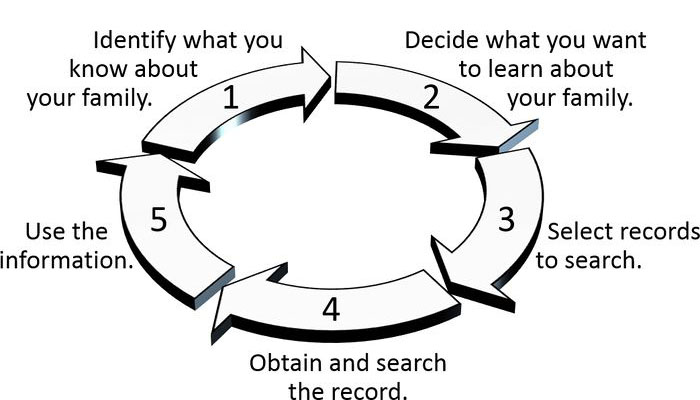
\includegraphics[scale=0.6]{02/researchProcess}
            \centering
            \caption{Procés de recerca genealògica.\label{fig:researchProcess}}
    \end{figure}

    \section{Conclusió}

    \paragraph{}
    Donem d'aquesta forma per conclosa la breu introducció a la genealogia. Com s'ha pogut observar, es tracta d'una ciència d'especial vocació personal, amb regulacions ambigües i rodejada de codis ètics i morals.

    Tot i les dificultats que tant genealogistes amateurs com professionals poden haver de fer front, aquesta ciència és capaç de desemmascarar i ajudar a comprendre les vivències dels nostres avantpassats i crear així un enllaç entre passat, present i futur. 


    \chapter{L'organització FamilySearch}
    \paragraph{}
    En aquest apartat de la memòria s'introduirà l’organització de FamilySearch. En concret, s’explicaran els objectius i motivacions sota les que va néixer l’organització, la seva història i el conjunt de funcionalitats i serveis que ofereixen a través del seu portal web i centres d’investigació.

    \section{Què és FamilySearch?}

    \paragraph{}
    Si haguéssim de resumir l’organització en una sola paraula, aquesta seria família. Com s’indicava en la introducció, FamilySearch és una organització sense ànim de lucre destinada  connectar famílies a través de diferents generacions. Des de l’organització es creu que les famílies són un condicionador de la felicitat i un dels factors que donen sentit a la vida.

    La seva visió com a empresa, amb les seves pròpies paraules, és:

    \begin{displayquote}
        Aprendre dels nostres avantpassats, a través dels llaços familiars, ens ajudà a comprendre millor qui som, enllaçar el present amb el passat i construir els ponts cap al futur.
    \end{displayquote}

    Aquesta visió és perseguida mitjançant un equip de professionals i voluntaris que treballen de cara a preservar i compartir el que s'ha convertit en la col·lecció més gran del món d'arxius genealògics. Aquest fet no és fruit de la casualitat, sinó dels més de cent anys que aquesta organització porta recol·lectant, preservant i compartint arxius genealògics des de tots els indrets del globus terraqüi.

    FamilySearch organitza i tracta els recursos disponibles tenint present que la finalitat de les dades és poder ser consumides per tercers. Per això, FamilySearch aposta per un model de dades eficaç, on aquelles persones interessades a explorar el seu passat, puguin descobrir amb certa facilitat quin són els seus orígens.

    Algunes de les característiques o dades que ajuden a comprendre l'envergadura i èxit d’aquesta organització se citen a continuació:

    \begin{itemize}
        \item Servei gratuït.
        \item Més de 4 bilions de persones diferents emmagatzemades en el sistema. Per tenir una idea de la magnitud d'aques nombre, actualment s’estima que en el món viuen 7,4 bilions de persones.
        \item 4.765 centres d’investigació distribuïts arreu del món.
        \item Servei d'ajuda 24/7.
    \end{itemize}

    \section{La història de FamilySearch}

    \paragraph{}
    FamilySearch, en els seus orígens coneguda com la Societat Genealògica de Utah, va néixer de les mans de l'església de Jesucrist dels Sants dels Darrers Dies l'any 1894. Aquesta església també és coneguda avui en dia pel nom de l'església mormona.

    L’organització porta acumulats a les seves espatlles més de cent anys de recerca i preservació d’arxius històrics i genealògics. Durant aquest recorregut, FamilySearch s’ha associat amb més de 10.000 arxius i 200.000 voluntaris de tota mena d’indrets.

    Mitjançant l’esforç col·lectiu d’aquestes organitzacions s’ha aconseguit preservar tant índexs com imatges d’arxiu de gran qualitat i posar tots aquests recursos a la disposició de milions de persones de forma gratuïta.

    Durant aquest trajecte de més de 100 anys iniciat l'any 1894, l'organització ha tingut l'oportunitat de celebrar grans èxits. Entre ells, destaquen els següents:

    \begin{itemize}
        \item \textbf{1938, Microfilm:} La societat genealògica de Utah és pionera en començar a utilitzar microfilm per filmar i emmagatzemar informació relativa a arxius genealògics arreu del món.
        \item \textbf{1942, Family group record archive:} Es crea, de forma manual, una indexació de les genealogies compartides fins aquell moment.
        \item \textbf{1963, Baül d’arxius a les Granite Mountains:} Es completa la creació d’un baül d’arxius amb tecnologia punta situat a les muntanyes pròximes a Salt Lake City, Utah, indret on resideix, avui en dia, la seu de l’organització. Es tracta d’una instal·lació climatitzada que ha estat utilitzada des de la seva creació per preservar còpies de microfilm i arxius digitals de més de cent països diferents.
        \item \textbf{1970, Primers centres d'història familiar:} S'introdueixen els primers centres d'història familiar. Aquests centres formen part d'una ramificació de llibreries que ofereixen accés gratuït a la informació continguda per més de 2,4 milions d'arxius en microfilm. Com hem esmentat en l'apartat anterior, avui en dia existeixen 4.765 d'aquests centres.
        \item \textbf{1985, L’estàndard GEDCOM:} En aquest any FamilySearch introdueix l'estàndard de \gls{GEDCOM}. L'estàndard GEDCOM consisteix en un conjunt d'especificacions i regles sobra com s'ha d'estructurar la informació genealògica de cara a compartir-la amb facilitat a través del núvol.
        \item \textbf{1995, Arbres genealògics digitalitzats:} Es dóna l’oportunitat als genealogistes de digitalitzar els arbres genealògics a la seva disposició i habilitar-ne l’accés a altres usuaris.
        \item \textbf{1998, Digitalització d’imatges:} FamilySearch comença a utilitzar tecnologies d'imatge digital per tal de capturar noves fonts de dades i transformar els milions de continguts, emmagatzemats fins ara en microfilm, en imatges digitals. La tecnologia també permet crear índexs de fàcil utilització que relacionen persones amb els continguts digitals.
        \item \textbf{1999, Nova pàgina web:} La pàgina web FamilySearch.org arriba al núvol. En la seva fase inicial, aquesta oferia la possibilitat de cercar informació en els registres històrics de forma relativament simple.
        \item \textbf{2012, Noves tecnologies digitals:} S’incorpora a les tecnologies utilitzades per FamilySearch la tecnologia dCamX, utilitzada per la digitalització de documents i la creació de  sales de lectura digital, responsables de facilitar les tasques de comunicació i alliberació de coneixement entre els diferents centres.
    \end{itemize}

    Un dels altres grans èxits de  l’organització, del que malauradament no es coneix la data exacte de creació, va ser \textbf{l’obertura de la FamilySearch \gls{API}.}

    Aquesta va suposar que aplicacions externes poguessin connectar-se a les bases de dades de FamilySearch i utilitzar-ne la informació d'una forma regulada i eficient. Resulta prou evident que sense l'existència d'aquesta \gls{API}, aquest projecte mai hagués pogut tenir lloc.

    \section{L'església mormona i la família}

    \paragraph{}
    Ja que el principal benefactor de FamilySearch és l'església mormona, creiem que és interessant estudiar de forma breu els orígens d'aquesta.

    L’església de Jesucrist dels Sants dels Darrers Dies és una església que considera que la religió hauria de tornar als seus inicis apostòlics. Va ser fundada pel nord-americà Joseph Smith el 6 d’abril del 1830, a l'oest de Nova York.

    Considerada actualment com la quarta comunitat cristiana més gran als Estats Units, troba situada la seva seu en l'actualitat a Salt Lake City, Utah. No obstant això, durant els inicis de l’església, Smith tenia la intenció de crear la Nova Jerusalem a prop de Nova York, en una ciutat que anomenaria \emph{Zion}.

    L’església, amb origen als voltants de Nova York, es va desplaçar cap a Kirtland, Ohio, des d'on va començar a expandir-se per Jackson County, Missouri, terra en què Smith volia situar la seu del col·lectiu en un futur pròxim.

    Joseph va veure contrariats els seus plans, quan l'any 1833, els colons van expulsar brutalment al col·lectiu de Missouri. Com que no disposaven dels recursos militars necessaris per recuperar el territori per la força, es van veure obligats a anar desplaçant-se al llarg de diferents localitzacions, sempre per culpa de conflictes amb els natius de les terres, fins a establir-se a Nauvoo, Illinois.

    Després de la mort de Smith, per tal d'evitar els conflictes armats amb els residents d'Illinois, el col·lectiu es va desplaçar cap a Nebraska i més endavant, durant l'any 1847, a les terres que serien conegudes com a Utah.

    Durant aquesta època, l'església es va veure sotmesa a grans pressions i crítiques a causa de la seva tolerància per la poligàmia. Les tensions entre el col·lectiu i el govern d'Estats Units anirien en augment, fins que l'any 1890, el congrés va disgregar l'església i es va apoderar de molts dels seus béns.

    Arribats aquest punt, l'església fundada per Smith, va decidir deixar de donar suport als matrimonis plurals, però sense desfer les famílies que ja es trobaven unides sota aquestes condicions.

    Durant el segle XX, l'església va créixer substancialment i es va veure sotmesa a un procés d'internacionalització, en gran mesura, gràcies a la feina dels missioners enviats a diferents indrets del món.

    Durant aquest període el col·lectiu es va convertir en un ferm defensor de les famílies nuclears, és a dir, de les famílies que consisteixen en dos progenitors i la seva descendència. L'església també va oposar-se en aquesta època a l'esmena pels drets igualitaris entre homes i dones, els casaments entre persones del mateix sexe i l'eutanàsia.

    Hem volgut redactar aquests paràgrafs previs sobre els orígens de l'església mormònica per tal de poder presentar, amb cert rigor històric, com l'església va veure canviat i evolucionat el concepte de família al llarg del temps.

    També queda latent, d'aquesta forma, com la història del col·lectiu es va veure marcada pel rebuig i el desterrament de moltes terres, fins al punt que van haver de recórrer a l'ús de missioners, repartits arreu del món, per tal de sobreviure com a religió.

    Així doncs, creiem que per aquest projecte no esdevé necessari entrar en més detall pel que fa a les doctrines i pràctiques de l'església, ni  enumerar quines són les principals diferencies entre l'església mormona i les altres corrents del cristianisme. Per altra banda, sí que volem realitzar una reflexió final sobre la posició actual de l'església mormona respecte a la família.

    Pels mormons, les famílies representen els lligams que uneixen a les persones en relacions personals i les connecten tant amb les passades com amb les futures generacions. Creuen que cap èxit en la vida, pot compensar el fracàs en l'àmbit familiar.

    Segons el seu punt de vista, construir nuclis familiars units i forts és el remei a molts dels fracassos que tenim les persones com a societat i creuen que la família inspira a l'individu a pensar més enllà de l'interès propi o la gratificació immediata i l'anima a entregar-se per altres persones, comunitats i a déu.

    Forma part també de la cultura mormona la pràctica o deure d'acumular i preservar, tant les històries dels seus avantpassats com les pròpies, en benefici d'aquells que encara estan per arribar, enllaçant, d'aquesta forma, generacions desconnectades d'una altra forma.

    Entenen la naturalesa real de la família, com un algú que transcendeix l'aquí i l'ara i que permet a les persones extreure forces d'aquells que van viure abans que nosaltres.

    Concloïen, si ajuntem les dues variables que van marcar l'esdevenir de l'església mormona fins als temps contemporanis, és a dir, la seva semi forçada internacionalització i la importància del nucli familiar en la seva cultura, no hauríem de mostrar-nos sorpresos pel fet que el col·lectiu s'hagi convertit en un dels referents mundials en el camp de la genealogia.

    \section{Serveis per organitzacions amb arxius genealògics}

    \paragraph{}
    Com ja s’ha comentat en seccions anteriors, FamilySearch no és només una organització dedicada a posar a disposició del públic registres genealògics, sinó que també pretenen ajudar a altres organitzacions a digitalitzar i publicar els seus documents al núvol de forma econòmica, ja sigui mitjançant la plataforma FamilySearch o la construcció de noves eines pròpies al núvol.

    Sigui com sigui, FamilySearch ofereix cinc serveis a altres organitzacions genealògiques:


    \subsection{Captura d'imatges}

    \paragraph{}
    Obtenir imatges de qualitat és normalment el procés més costos per aquelles organitzacions que volen digitalitzar els seus registres, tant en el sentit econòmic, com en base als recursos humans necessaris.

    El microfilm, que fins fa poc era l’estàndard en la indústria, comença a cedir pas al món digital i tant si l’objectiu de les organitzacions és digitalitzar el seu contingut mitjançant medis propis o utilitzant la tecnologia disponible en els centres de recerca de FamilySearch, aquests ofereixen la seva ajuda a les organitzacions que la sol·licitin.

    La tecnologia dCamX, utilitzada per FamilySearch, es caracteritza per la creació d'imatges d’alta qualitat, de forma eficaç, al mateix temps que es capturen meta dades de la imatge. Aquest aspecte, conjuntament amb un procés de publicació posterior fàcil i ràpid, fan que aquesta tecnologia estigui cridada a ser el nou estàndard a la indústria.


    \subsection{Conversió de formats digital}

    \paragraph{}
    Aquest servei està pensat per aquelles empreses o organitzacions que ja disposen d’una elevada quantitat de material en format de microfilm.

    La tecnologia digital ha canviat dràsticament com els registres són capturats, emmagatzemats i fets accessibles. Aquesta tecnologia segueix progressant i per tant resulta indispensable començar a adaptar-se al més aviat possible.

    FamilySearch posa a disposició de les organitzacions genealògiques la possibilitat d’utilitzar els mateixos processos i software que utilitzen ells per digitalitzar la seva col·lecció de més de 2,4 milions de microfilms. FamilySearch, també ofereix la possibilitat d’emmagatzemar els fitxers digitals d’aquestes organitzacions en els seus servidors, un cop convertits, si així ho prefereixen.


    \subsection{Indexació en línea}

    \paragraph{}
    Un cop un registre ha estat digitalitzat en forma d’imatge, la informació principal necessita ser extreta i transcrita per tal de poder produir índexs sobre els quals clients o usuaris puguin cercar.

    L’aplicació d’indexació en línea, creada per FamilySearch, permet, mitjançant la cadena de voluntaris, crear índexs de forma ràpida i precisa. Els arxius de les organitzacions, que així ho sol·licitin, podran disposar d’accés a aquesta cadena de voluntaris per digitalitzar els seus índexs o accés a les eines d’indexació auxiliars  que permeten la creació de projectes propis.


    \subsection{Accés en línea}

    \paragraph{}
    Si un document o registre no esdevé fàcilment accessible, resulta de poc valor pels usuaris. FamilySearch ofereix dos serveis diferents depenent de si les organitzacions desitgen fer públic l'accés a les seves dades a través de FamilySearch.org o no.

    En cas de voler per públics els registres, FamilySearch s’ofereix a penjar i mantenir els registres de forma econòmica. En cas de voler mantenir els registres en un àmbit privat, l’organització posa a disposició dels interessats les eines i experiència necessàries per crear un espai propi al núvol.


    \subsection{Preservació dels registres i fitxers físics}

    \paragraph{}
    FamilySearch ofereix l’opció a les organitzacions de custodiar còpies de seguretat dels seus fitxers, en el baül de tecnologia punta situat a las Granite Mountains. En l'actualitat, còpies d’arxius de microfilm i digitals, provinents de més de cent països diferents, es troben guardades en aquest baül per precaució.

    El fet de disposar de còpies de seguretat pels fitxers genealògics, suposa la salvació de registres en cas de terratrèmols, incendis, inundacions, tornados, guerres i actes humans no controlables en les seus oficials dels arxius.

    Les mesures de seguretat que FamilySearch utilitza pels seus registres i que a la vegada, queden a disposició d’altres organitzacions, són:

    \begin{itemize}
        \item Processos complets i automatitzats de comprovació, validació i actualització dels registres per garantir la màxima protecció possible.
        \item Migració gradual i eficient de registres cap a noves tecnologies quan els formats previs quedin obsolets, garantint així la seva accessibilitat a llarg termini.
        \item Processos de conversió i preservació de dades que compleixen amb les regulacions sobre els \gls{OAIS}.
        \item Col·leccions d’informació emmagatzemada al núvol i distribuïdes en diferents clústers arreu del món per garantir una alta capacitat d’emmagatzematge, escalabilitat i protecció contra els desastres.
        \item Utilització de les últimes tecnologies en el tractament de dades d'alta densitat.
        \item Procés ràpid i eficient de cara a processar l'arribada de nous registres al sistema. El sistema actual és capaç de processar més de vint terabytes al dia, mesura que incrementa, al mateix temps que la tecnologia avança.
        \item Servidors configurats en clústers virtuals per garantir una escalabilitat infinita.
        \item Facilitat amb control climàtic, prevenció de focs, fonts d’energia auxiliars per casos d’emergència i replicació d’arxius digitals.
    \end{itemize}


    \subsection{Conclusions sobre els serveis professionals}

    \paragraph{}
    En els apartats anteriors s'ha pogut observar com FamilySearch està clarament interessada a posar les seves tecnologies a disposició d'altres organitzacions genealògiques.

    Aquesta estratègia de col·laboració els permet incorporar a les seves bases de dades registres d'informació, d'altre forma inaccessibles i garantir la persistència de les dades davant d'esdeveniments no controlables, d'informació gestionada per altres organitzacions.


    \chapter{Introducció a l'API de FamilySearch}

    \section{El portal de desenvolupadors}

    \paragraph{}
    Tota la informació disponible per tal de poder començar a familiaritzar-se amb l’\gls{API} de FamilySearch, pot ser trobada en el portal de desenvolupadors.

    Aquest apartat de la web està format per diferents seccions, malauradament, l’estructura no acaba de resultar del tot clara per una persona que vulgui iniciar-se per primer cop en l'ús d'aquesta \gls{API}.

    Si ens enfoquem més en la documentació disponible, que no pas en l'estructura proposada per l’organització, podem veure que la informació es podria distribuir, en certa forma, en els següents grups:

    \begin{itemize}
        \item \textbf{Requisits tècnics:} Conjunt d’informació necessària per comprendre l’estructura de l'\gls{API}, els formats de dades que maneja i els passos necessaris per començar a interactuar amb aquesta.
        \item \textbf{Recursos disponibles i rutes d’accés:} Informació detallada sobre cada recurs accessible a través de l'\gls{API}. En concret, disposa dels detalls de com accedir al recurs, les operacions que es poden realitzar sobre ell, la informació que conté i quines són les connexions amb altres recursos.
        \item \textbf{Evolució i canvis produïts a l'\gls{API}:} Informació semi ordenada de com l'\gls{API} s’ha vist evolucionada al llarg del temps i un recull dels canvis produïts sobre els recursos, procés de certificació, material de documentació i eines de desenvolupament.
        \item \textbf{Serveis extres oferts per l'\gls{API}:} Aquest recull d’articles conceptualitza característiques de l'\gls{API} com poden ser els recursos d'\emph{emmagatzematge}, \emph{localització} o \emph{throttling}.
        \item \textbf{Eines de desenvolupament:} Recull d’entorns de desenvolupament i eines extres que poden facilitar la feina del desenvolupador.
        \item \textbf{Certificació:} Recull la informació necessària per gestionar els diferents processos de certificació i informació sobre les regulacions a les quals s'ha de fer front en cas de voler certificar l'aplicació.
    \end{itemize}

    \section{L'arquitectura de l'\gls{API}}


    \subsection{Què és una \gls{API}?}

    \paragraph{}
    Abans d'entrar en detall en com funciona una \gls{API}, estaria bé definir, amb una mica més de precisió, en què consisteix exactament.

    Una \gls{API}, de l'anglès `Application Programming Interface' o Interfície de programació d'aplicacions en català, representa el conjunt de subrutines, funcions i procediments que ofereix una biblioteca per tal de ser utilitzada en el software de tercers com una capa d'abstracció. Aquest conjunt de subrutines, funcions i procediments, acostumen a oferir accés a certs serveis o conjunts de dades d'un particular, a tercers, de forma controlada.


    \subsection{L'arquitectura REST}

    \paragraph{}
    L’arquitectura sobre la qual està creada l’\gls{API} de FamilySearch és una arquitectura REST. Les sigles provenen de l’anglès i representen el concepte: \gls{REST}.

    Les arquitectures \gls{REST} es caracteritzen per estar orientades els recursos més que a les accions que es poden realitzar sobre ells i com a peculiaritat, es caracteritzen per sis regles o restriccions.

    Aquestes són: interfície uniforme, sense estat, client-servidor, emmagatzemables, sistema per capes, i codi sota petició. Aquests sis conceptes són doncs els que defineixen les bases de es arquitectures \gls{REST}.

    És diu que una arquitectura \gls{REST} és orientada als recursos perquè estan construïdes al voltant d’objectes i les relacions entre aquests, en comptes d’accions. Per exemple, a l’\gls{API} de FamilySearch, es parla de persones i esdeveniments, en comptes de llegir persones o crear esdeveniments i en canvi, aquestes operacions, passen a formar part dels objectes \emph{Persona} i \emph{Esdeveniment.}

    L'intercanvi de dades es produeix mitjançant l'ús de diferents representacions. Aquestes, expliquen com els recursos són tractats per l’\gls{API} i de quina forma han de ser realitzades les comunicacions entre el servidor i el client. Els formats més freqüents són JSON i XML. FamilySearch ofereix suport per ambdós formats.

    Per posar un exemple reduït que il·lustri el que estem explicant, podem descriure de la següent forma, el que podria ser una operació contra l'\gls{API} de FamilySearch, especificant quin element seria considerat el Recurs, quin el Servei i quin la Representació:

    \begin{itemize}
        \item \textbf{Recurs:} Persona (informació relacionada amb una persona en concret)
        \item \textbf{Servei:} Obtenir informació de la persona (GET)
        \item \textbf{Representació:} Nom, cognoms, esdeveniments relacionats amb la vida de la persona, etcètera, en format \gls{XML} o \gls{JSON}.
    \end{itemize}

    \paragraph{}
    Com també s'ha comentat, l’arquitectura \gls{REST} es caracteritza per la implementació de sis restriccions imposades sobre el sistema. A continuació s'exposa amb més detall, cada una d'elles.


    \subsubsection{Interfície uniforme (uniform interface)}

    \paragraph{}
    Aquesta restricció s'encarrega de definir la interfície de comunicació entre el client i el servidor.

    En una arquitectura REST, s'utilitzen els protocols de comunicació \gls{HTTP} i \gls{HTTPS} de forma conjunta amb els \gls{URI}, per aconseguir accés als diferents recursos i operacions proporcionades per l'\gls{API}.

    Els verbs permesos pels protocols de comunicació web són els coneguts: get, put, post, delete, options and head.

    Per exemple, per fer la petició de lectura sobre el recurs d’una Persona a l’\gls{API} de FamilySearch, executaríem la següent crida \gls{HTTP} o \gls{HTTPS} mitjançant el verb i URI especificats a continuació:\\ \verb|GET /platform/genealogies/persons/2:2:PPPJ-MYZ7|.


    \subsubsection{Sense estat (stateless)}

    \paragraph{}
    Aquesta restricció implica que el servidor no emmagatzema la informació del client. Això implica que cada petició d'aquest cap a l’\gls{API}, ha de contenir tota la informació necessària perquè el servidor l'identifiqui i es defineixin les regles de comunicació adequades per processar la petició.

    Hi ha exemples d'operacions a l'\gls{API} de FamilySearch, com per exemple el procés d'identificació Oauth V2, que no són realment RESTful, doncs aquestes sí que guarden informació del client durant les diferents parts de la comunicació.


    \subsubsection{Client-servidor (client-server)}

    \paragraph{}
    Per comprendre aquesta restricció, cal comprendre primer en què consisteix un sistema desconnectat.

    En el cas de les arquitectures REST, un sistema desconnectat implica que el client mai tindrà accés directe a les bases de dades que emmagatzemen la informació, i que per tant, sempre haurà d'accedir a les dades mitjançant l’intermediari. En aquest cas, l'\gls{API}.

    Els protocols de comunicació descrits prèviament (\gls{HTTP} i \gls{HTTPS}), i la interfície de comunicació, són els encarregats de gestionar les comunicacions entre client i servidor.


    \subsubsection{Emmagatzematge en el client (cacheable)}

    \paragraph{}
    Aquesta restricció fa referència a si les respostes retornades, des del servidor, al client, poden ser emmagatzemades per aquest i durant quant de temps les pot guardar. Existeixen tres nivells de configuració diferents:

    \begin{itemize}
        \item \textbf{Implícit:} Si és el client el que decideix quant de temps guardarà les dades o informació retornada, es tracte d'emmagatzematge implícit.
        \item \textbf{Explícit:} Si és el servidor el que mana i posa les regles, parlem d'emmagatzematge explícit.
        \item \textbf{Negociat:} Quan el client i el servidor negocien i arriben a un acord, es tractea d'emmagatzematge negociat.
    \end{itemize}


    \subsubsection{Sistema per capes (layered system)}

    \paragraph{}
    Aquest principi, o restricció, es basa en el fet que el client no pot assumir que tindrà connexió directa amb el servidor. És a dir, poden existir diferents intermediaris en forma de hardware i software entre client i servidor.

    Això, facilita l’escalabilitat i persistència del sistema gràcies al fet que el client no s’ha de preocupar de comunicar-se amb elements o tecnologies específiques. D'aquesta forma, el servidor es pot veure subjectes a canvis de forma transparent pels clients.


    \subsubsection{Codi sota petició (code on demand)}

    \paragraph{}
    Restricció que regula com, de forma excepcional, el servidor pot proporcionar accés al client sobre certes parts de la lògica del funcionament. Alguns exemples poden ser els \emph{Java Applets} o blocs de codi \emph{JavasScript}.

    \section{Formats de dades utilitzats pel Sistema}

    \paragraph{}
    FamilySearch utilitza tres formats de dades diferents per representar la informació emmagatzemada en les seves bases de dades i dos formats extres per codificar aquesta informació i enviar-la a través del núvol.

    Els conjunts de dades utilitzats per representar els recursos són els que segueixen:

    \begin{itemize}
        \item Les dades genealògiques es representen mitjançant el format GEDCOM X.
        \item Els recursos o objectes específics del model de FamilySearch, es representen mitjançant una extensió del model de dades GEDCOM X.
        \item El format de dades Atom, o atòmic, s’utilitza per proporcionar un format simple per les meta-dades.
    \end{itemize}


    \subsection{El format de dades GEDCOM i GEDCOM X}

        \paragraph{}
        El terme \gls{GEDCOM}, és un acrònim de l'anglès Genealogical Data Communications.

        El format GEDCOM consisteix en un conjunt de regles d'aplicació per tal de representar informació genealògica. Aquest format de dades, creat per FamilySearch l'any 1984, s'ha convertit en l'estàndard de la indústria.

         Per simplificar-ho, podríem entedre un fitxer en format GEDCOM, com un fitxer de text que emmagatzema informació genealògica d’una persona i les metadades necessàries per poder enllaçar als diferents fitxers de la mateixa persona.

         Tot i que l’última versió, datada del 1996, segueix sent molt utilitzada, FamilySearch va proposar durant l'any 2012, canviar aquest estàndard per la seva nova versió anomenada GEDCOM X.

         El format de dades per la \gls{GEDCOM X}, representava un nou projecte de codi obert i es diferenciava del seu antecessor en la implementació d'un sistema que facilitava la inclusió d'arbres genealògics i fonts de dades als recursos ja existents.

         Al mateix temps, el nou estàndard també donava suport a l'intercanvi i enllaçament de dades a través del núvol i es creava així la primera versió de l'API de FamilySearch.

         A continuació, a la taula [ref] s'ofereix un petit exemple de com un recurs és codificat part del recurs persona sota el format de dades GEDCOM X.

        \begin{center}
                 \csvreader[
                    separator=comma,
                    before table=\sffamily\small,
                    longtable={p{1.5cm-2\tabcolsep}p{4.5cm-2\tabcolsep}p{4.5cm-2\tabcolsep}p{3.5cm-2\tabcolsep}},
                    table head={\toprule%
                        \headentry{m{1.5cm-2\tabcolsep}}{Nom}
                        & \headentry{m{4.5cm-2\tabcolsep}}{Desc.}
                        & \headentry{m{4cm-2\tabcolsep}}{Format}
                        & \headentry{m{4cm-2\tabcolsep}}{Rest.}\\\midrule},
                    late after line=\\\midrule,
                    late after last line=\\\bottomrule,
                 ]
                 {./tables/04/gedcomFinal.csv}
                 {nom=\nom,desc=\desc,format=\format,rest=\rest}
                 {\nom&\desc&\format&\rest}
         \end{center}

         \paragraph{}
         Així doncs, podem veure com la instància del recurs Persona conté un camp booleà, que indica si aquesta pot ser utilitzada de forma pública o només en l'àmbit privat i tres camps que es troben codificats sota els estàndards del format GEDCOM X.

         Per exemple, el format de dades \verb|http://gedcomx.org/v1/Gender|, representaria un recurs amb l’estructura que s’exposa a la taula [ref2] i els valors possibles per l’enumeració de gènere, s’indiquen en la taula [ref3]

         [TABLE 2]

         [TABLE 3]

         \paragraph{}
         Com que l’objectiu del projecte no és estudiar la codificació GEDCOM o GEDCOM X, sinó comprendre quina informació es troba realment disponible a través de l'API de FamilySearch, no entrarem més en detall en aquests formats.

         L’objectiu d’aquest apartat era explicar quin és l'estàndard de representació de dades genealògiques utilitzat per l'API. Per qualsevol informació extra que es vulgui consultar, s’adjunta a la bibliografia del projecte, l’enllaç a la documentació del model conceptual.


     \subsection{Format de dades FamilySearch}

        \paragraph{}
        El format de dades FamilySearch, defineix el format d'aquells objectes específics relacionats amb la plataforma de dades pròpia de l'organització. Això implica que aquestes estructures no formen part de cap estàndard i manquen de sentit fora del context pel qual han estat definides.

        L'estructura dels objectes específics de FamilySearch ha estat creada com una extensió de l'especificació GEDCOM X. Per tant, segueixen una estructura molt similar.


    \subsection{Format de dades Atom (o Atòmic)}

        \paragraph{}
        Els formats de dades Atom, o atòmic, és utilitzat per proporcionar un format pel contingut web i les metadades.

        Aquest format és utilitzat, entre altres llocs, en les col·leccions ordenades de resultats, com podrien, per exemple, les respostes a la funció de cerca de persones o l'obtenció del historial de canvis d’una persona.


    \subsection{Codificacions dels formats de dades}

        \paragraph{}
        Els formats de dades que s’han exposat en els apartats anteriors no són més que unes convencions que marquen l'estructura a seguir per representar els diferents objectes o recursos utilitzats per l'API de FamilySearch.

        Tanmateix, aquestes estructures han de ser codificades per tal de poder ser transmeses a través del núvol i en concret, FamilySearch, proporciona suport a les dues codificacions més comunes i utilitzades per aquesta finalitat. Els llenguatges XML i JSON.


        \subsubsection{El llenguatge XML}

        \paragraph{}
        El \gls{XML}, és un llenguatge de marcatge que defineix un conjunt de regles a seguir per tal de codificar, documents i informació, en un format llegible i processable, tant per éssers humans, com màquines.

        El llenguatge va ser definit pel Consorci World Wide Web i tracta d’emfatitzar la simplicitat, generalitat i usabilitat del model, per l'ús a través d'Internet.

        Una versió reduïda de la representació en XML del recurs ‘Nota’, amb camps: subjecte, text i atribució, quedaria representat de la forma següent:

        \begin{lstlisting}[style=rawOwn,caption={Representació bàsica en XML d'una Nota}]
<Note xmlns='...'>
    <subject>...</subject>
    <text>...</text>
    <attribution id='...'>
        <contributor resourceId='...' resource='...'/>
        <modified>...</modified>
        <changeMessage>...</changeMessage>
        <creator resourceId='...' resource='...'/>
        <created>...</created>
    </attribution>
</Note>
        \end{lstlisting}

        \paragraph{}
        Com es pot observar, cada camp, objecte o peça d'informació, es troba envoltada per dues etiquetes que en marquen l'inici i final. El text situat a l'interior d'aquestes etiquetes, indica de quin camp es tracta. Per exemple, pel camp subjecte, tenim les etiquetes \emph{<subject>} i \emph{</subject>}.


        \subsubsection{El llenguatge JSON}

        \paragraph{}
        El llenguatge \gls{JSON}, és un estàndard de format obert que, de la mateixa forma que el llenguatge XML, pretén crear codificacions llegibles tant per éssers humans com màquines i al mateix temps, poder transmetre aquestes dades a través del núvol de forma ordenada.

        Aquest format es basa en el concepte ‘clau -valor’. És a dir, cada camp d'un objecte a representar està format per una clau i un valor associat a aquesta clau.

        El llenguatge JSON deriva del JavaScript. Al principi, només aquesta plataforma incorporava funcions per codificar i descodificar aquest llenguatge de marcatge.

        Durant els últims anys, el format JSON s'ha vist convertit en l'estàndard de la indústria per l'intercanvi de dades a través d'Internet i en conseqüència, ha provocat que molts altres llenguatges de programació hagin incorporat les seves pròpies funcions de codificació i descodificació.

        Una versió reduïda de la representació en JSON del recurs Nota, amb camps: subjecte, text i atribució, es representaria de la forma següent:

        \begin{lstlisting}[style=rawOwn,caption={Representació bàsica en JSON d'una Nota}]
{
  `lang': `...',
  `subject': `...',
  `text': `...',
  `attribution': {
    `contributor': { },
    `modified': `...',
    `changeMessage': `...',
    `creator': { },
    `created': `...',
    `id': `...'
  },
  `id': `...'
}
        \end{lstlisting}

    \section{Evolució temporal de l'API}

    \subsection{Evolucions al llarg del temps}

    \paragraph{}
    


    \chapter{Estudi en profunditat de l'API de FamilySearch}

    \section{Els recursos de FamilySearch}

    \paragraph{}
    L'API de FamilySearch organitza tota la informació disponible en objectes que són anomenats recursos.

    Cada recurs emmagatzema informació relativa al concepte que representen. Per exemple, el recurs Persona conté informació sobre si aquesta està viva o morta, el seu nom i tota mena d'informació i esdeveniments relacionats amb la seva vida.

    En la taula~\ref{ref:personGedcom} de la secció anterior de la memòria, observàvem ja com a exemple alguns dels paràmetres continguts pel recurs Persona de l'API de FamilySearch.

    El recursos també es caracteritzen per emmagatzemar informació relativa a quines operacions es poden realitzar sobre ells. Per exemple, el recurs Persona conté informació sobre com accedir a les operacions llegir una persona, editar una persona, esborrar una persona, buscar possibles duplicats de la persona, etcètera.

    Finalment, els recursos també destaquen per contenir els enllaços o més ben dit, les URIs, als recursos relacionats. Parlarem més en detall d’aquestes URI en el següent apartat de la memòria.

    \section{Enllaços hypermedia, la navegació entre recursos}

    \paragraph{}
    Com hem comentat en l’apartat anterior, els recursos emmagatzemen informació sobre les URI dels recursos relacionats. Aquestes URI són anomenades enllaços hypermedia i permeten la navegació  entre els diferents recursos del model de dades.

    Per posar un exemple, imaginem el recurs Persona. Aquest conté enllaços hypermedia que apunten als recursos que conformen el concepte Parella, Pares, Fills, Fonts d'informació, Ascendència, Descendència i Memòries. Cada un d'aquests recursos apuntats conté informació específica i d'interès respecte a la persona consultada.

    La figura~\ref{fig:hypermedia} reflecteix com el recurs Persona és accessible a través de l'Arbre Familiar de FamilySearch i com les diferents relacions i recursos, associats a una persona, són connectats a través dels enllaços hypermedia d'aquest.

    \begin{figure}[h]
        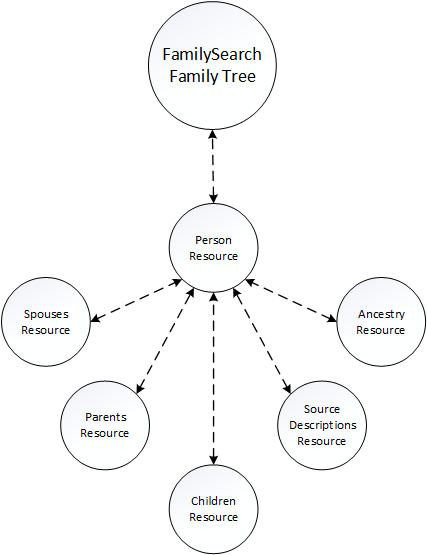
\includegraphics[scale=0.8]{05/01_hypermedia}
        \centering
        \caption{Enllaços hypermedia del recurs Persona.}\label{fig:hypermedia}
    \end{figure}

    Volem aprofitar aquest apartat de la memòria per recordar, que en el moment en què la nova versió del back-end, Family Tree, es trobi desplegada per complet a producció, el recurs Persona no contindrà més els enllaços hypermedia a tots aquests recursos, sinó que les relacions de parella o paternals, es trobaran incloses dins del mateix recurs Persona.

    De totes maneres, el concepte dels enllaços hypermedia seguirà sent vàlid de cara a les relacions del recurs Persona amb la resta de recursos vinculats i per tota la resta de relacions entre els diferents recursos de l'API de FamilySearch.

    Els enllaços hypermedia cobren especial interès a l'hora de crear aplicacions robustes que es vegin el menys afectades possible per canvis en la localització o crida dels recursos.

    El primer gran avantatge d’utilitzar aquests enllaços és que no cal implementar en el codi, de forma específica, les URI d'accés a cada recurs. D'aquesta forma, s'aconsegueix evitar que en cas de canvis en les URI, sigui necessari realitzar modificacions en el codi de les nostres aplicacions.

    El segon, és que si es coneix un sol punt d’entrada al sistema, les aplicacions ja no requeriran més informació per tal de navegar entre els diferents recursos de la resposta. D'aquesta forma, podríem descriure els enllaços hypermedia com una espècie d'índexs que permeten explorar i navegar a través del conjunt de recursos que conformen les respostes de l'API de FamilySearch. 

    \section{L'arbre genealògic de FamilySearch}

    \paragraph{}
    El model de dades que conforma l'arbre genealògic de FamilySearch, consta de molts recursos i enumeracions diferents. No citem en la memòria el nombre total de recursos diferents, ja que alguns dels objectes documentats de forma oficial es troben en desús, mentre que alguns objectes nous, encara no han rebut la documentació pertinent.

    El conjunt d'objectes o recursos connectats, conformen el que ha estat enomenat l'arbre familiar de FamilySearch (Family Tree). Aquest arbre, pot ser subdividit en cinc grans blocs:

    \begin{itemize}
        \item \textbf{El bloc de persones:} Aquest bloc representa al conjunt de recursos que emmagatzemen la informació personal de les diferents persones representades a l'arbre familiar.
        \item \textbf{El bloc de les relacions familiars:} Aquest bloc està format per aquells recursos que contenen informació sobre les diferents relacions familiars entre les persones emmagatzemades en el sistema.
        \item \textbf{El bloc de col·leccions:} Aquest bloc recull els recursos que guarden la informació relativa a les fonts de dades i documents digitalitzats, que certifiquen la veracitat de les dades.
        \item \textbf{El bloc de discussions:} El bloc de discussions conté aquells recursos que contenen la informació relativa a les converses o discussions creades, per part dels usuaris, al voltant de les persones de l'arbre familiar.
        \item \textbf{El bloc de memòries:} Aquest últim bloc està format per aquells recursos que emmagatzemen la informació relativa a les memòries descrites en la secció tres d'aquesta memòria.
    \end{itemize}

    La imatge~\ref{fig:familyTree} mostra aquests cinc grans blocs que conformen l'arbre familiar de FamilySearch i com es troben relacionats entre ells.

    \begin{figure}[h]
        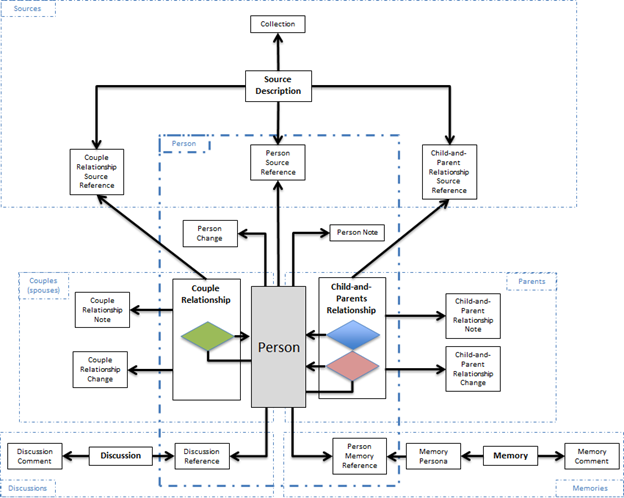
\includegraphics{05/02_overallModel}
        \centering
        \caption{Estructura de l'arbre familiar de FamilySearch}\label{fig:familyTree}
    \end{figure}

    Els blocs principals de l'arbre familiar són, sense cap mena de dubte, els que contenen la informació relativa a les persones i a les relacions familiars que les lliguen.

    L’objectiu de la resta de blocs que conformen l'arbre familiar és el de proporcionar suport i informació extra més detallada sobre les persones, relacions familiars, veracitat de les dades i investigacions realitzades sobre aquestes persones i línies genealògiques.

    En els següents apartats de la memòria s'estudiarà el conjunt de recursos principals que conformen cada bloc de l'arbre familiar i quines són les diferents peces d'informació accessibles a través de cada un d'aquests recursos.

    No es representarà en aquest projecte el conjunt total d'operacions diferents que pot ser realitzat sobre els diferents recursos, ja que les possibilitats de configuració d'aquestes són molt elevades i no té gaire sentit duplicar tota la documentació oficial respecte aquest punt.

    Tanmateix, sí que volem mencionar que gairebé tots els recursos que formen part del model de dades de FamilySearch, poden ser sotmesos als següents grups d'operacions:

    \begin{itemize}
        \item \textbf{Lectura:} Tots els recursos són, evidentment, llegibles. Cada un dels recursos conté diferents opcions de lectura i generalment, també solen ser personalitzables mitjançant la inclusió de diferents paràmetres.
        \item \textbf{Actualització:} Sempre que es disposi dels permisos adequats sobre les dades, els usuaris també poden realitzar operacions d'actualització per corregir errors, modificar la informació existent o bé afegir nova informació.
        \item \textbf{Esborrat:} Si es disposa dels permisos suficients, els usuaris poden esborrar informació incorrecta o duplicada dels diferents recursos, o el recurs sencer, mitjançant les operacions d'esborrat.
        \item \textbf{Creació:} En cas de voler afegir noves peces d'informació a les bases de dades de FamilySearch, siguin noves persones o informació específica relacionada a alguna persona que ja es troba en el sistema, això és realitzable a través de les operacions de creació de cada recurs.
    \end{itemize}

    Dit això, passem doncs a analitzar els principals recursos de cada bloc de l'arbre familiar i les peces d'informació més destacables que els conformen.

    \section{Recursos principals del bloc persones}

    \paragraph{}
    El centre d'aquest bloc de recursos és el recurs Persona. Aquest recurs, emmagatzema els detalls que identifiquen i caracteritzen a cada una de les persones de l'arbre així com la informació bàsica sobre els seus relatius més propers.

    D'aquest recurs principal, pengen els enllaços cap als recursos que permeten obtenir informació sobre els relatius de la persona, els estudis realitzats sobre aquesta, l'historial de canvis, les fonts d'informació i les memòries afegides pels usuaris.

    La imatge [ref] ofereix una visió de l'esquema que acabem de descriure i permet veure com el recurs Persona s'enllaça amb la resta de blocs que conformen l'arbre familiar~\ref{img:personsBloc}.

    \begin{figure}[h]
        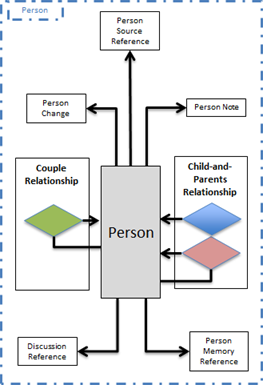
\includegraphics{05/03_personsCore}
        \centering
        \caption{El bloc de l'arbre familiar relatiu a les Persones.}\label{img:personsBloc}
    \end{figure}

    Aquest bloc de recursos és el més gran de tots i pràcticament, emmagatzema tota la informació rellevant dels individus accessibles a través de l'API. En els següents subapartats s'exposaran els diferents recursos que conformen aquest bloc i quines són les peces d'informació utilitzables que aquests contenen.

    Podreu observar, en les taules que representen l'estructura dels recursos, que a vegades, per la columna que marca el format de dades d'un paràmetre, aquest es troba especificat entre els caràcters `[' i `]'. Aquesta terminologia s'utilitza per indicar que aquest paràmetre és en realitat un recurs o objecte de dades diferent inclòs dins del recurs estudiat.

    També s'observarà que sovint, els recursos exposats, hereten dades d'altres recursos i en els casos que aquests siguin rellevants, se n'exposarà l'estructura a l'apartat `Altres recursos interessants', més endavant en la memòria.

    \subsection{El recurs Persona (Person)}

    \paragraph{}
    El recurs Persona és el primer objecte amb què cal familiaritzar-se per tal de comprendre la potencialitat emmascarada d'aquesta API.

    Cada instància, fa referència a una persona diferent de l'arbre familiar i generalment, representa el punt d'entrada per tal d'accedir a tota la informació disponible sobre un individu, ja sigui perquè aquesta es troba inclosa en el recurs o esdevé accessible a través dels enllaços hypermedia.

    Els enllaços hypermedia del recurs Persona permeten accedir a la informació relativa als seus avantpassats, descendents, artefactes, historial de canvis, parelles, discussions, notes i fonts de dades.

    Les dades pròpies pel recurs Persona poden ser observades a la taula~\ref{tab:person}. Cal recordar que aquest recurs també hereta els paràmetres dels recursos Subjecte, Conclusió, Enllaços Hypermedia i Dades Extensibles que poden ser trobats a la secció `Altres recursos interessants'.

    \begin{center}
             \csvreader[
                separator=comma,
                before table=\sffamily\small,
                longtable={p{2cm-2\tabcolsep}p{3.5cm-2\tabcolsep}p{8.5cm-2\tabcolsep}},
                table head={\caption{Codificació GEDCOM X del recurs Persona}\label{tab:person}\\\toprule%
                    \headentry{m{2cm-2\tabcolsep}}{Paràmetre}
                    & \headentry{m{3.4cm-2\tabcolsep}}{Format de Dades}
                    & \headentry{m{8.5cm-2\tabcolsep}}{Descripció}\\\midrule},
                late after line=\\\midrule,
                late after last line=\\\bottomrule,
             ]
             {./tables/05/01_persons/person.csv}
             {param=\param,format=\format,desc=\desc}
             {\param&\format&\desc}
     \end{center}

    \subsection{El recurs Gènere (Gender)}

    \paragraph{}
    El recurs Gènere s'utilitza per especificar el gènere d'una persona en concret. Aquest recurs conté els paràmetres propis mostrats a la taula~\ref{tab:gender} i hereta els camps de dades dels recursos , Conclusió, Enllaços Hypermedia i Dades Extensibles que poden ser trobats a la secció `Altres recursos interessants'.

    \begin{center}
             \csvreader[
                separator=comma,
                before table=\sffamily\small,
                longtable={p{2cm-2\tabcolsep}p{3.5cm-2\tabcolsep}p{8.5cm-2\tabcolsep}},
                table head={\caption{Codificació GEDCOM X del recurs Persona}\label{tab:gender}\\\toprule%
                    \headentry{m{2cm-2\tabcolsep}}{Paràmetre}
                    & \headentry{m{3.4cm-2\tabcolsep}}{Format de Dades}
                    & \headentry{m{8.5cm-2\tabcolsep}}{Descripció}\\\midrule},
                late after line=\\\midrule,
                late after last line=\\\bottomrule,
             ]
             {./tables/05/01_persons/gender.csv}
             {param=\param,format=\format,desc=\desc}
             {\param&\format&\desc}
     \end{center}


     \subsubsection{L'enumeració genderType}

     \paragraph{}
     L'enumeració genderType segueix l'estructura de definició GEDCOMX. Com a tal, els valors possibles per l'enumeració segueixen la pauta:\\\verb|http://gedcomx.org/ + `genderType'|

     La següent taula mostra els tres possibles valors de l'enumeració genderType.

     \begin{center}
         \csvreader[
            no head,
            separator=comma,
            table head={\caption{Valors possibles per genderType}\label{tab:genderType}},
            before table=\sffamily\small,
            longtable={|p{3cm}|p{3cm}|p{3cm}|},
            column count=4,
            late after head=\\\hline,
            late after line=\\\hline,
            late after last line=\\\hline,
         ]
         {./tables/05/01_persons/genderType.csv}
         {1=\one,2=\two,3=\three}
         {\one&\two&\three}
     \end{center}

    \subsection{Els recursos Nom, Forma del Nom i Part del Nom (Name, NameForm, NamePart)}

    \paragraph{}
    Aquest conjunt de recursos s'utilitza per representar la informació relativa als noms d'una persona.  Contenen informació sobre si un nom és el preferit de cara a ser utilitzat com a nom principal, en quin moment la persona va adoptar aquest nom i diferents formes de representació.

    Resulta útil poder accedir a diferents noms d'una mateixa persona, per poder així alternar, per exemple, entre el seu mot i el nom en el moment de naixement o defunció.

    El recurs Nom està format pels paràmetres mostrats a la taula~\ref{res:name} i hereta també els paràmetres dels recursos Conclusió, Enllaços Hypermedia i Dades Extensibles que poden ser trobats a la secció `Altres recursos interessants'.

    Per altre banda, els recursos Forma del Nom i Part del Nom, contenen els paràmetres mostrats a les taules~\ref{res:nameForm} i~\ref{res:namePart} respectivament i hereten els paràmetres del recurs Dades Extensibles descrit en l'apartat `Altres recursos interessants'.

    \begin{center}
             \csvreader[
                separator=comma,
                before table=\sffamily\small,
                longtable={p{2cm-2\tabcolsep}p{3.5cm-2\tabcolsep}p{8.5cm-2\tabcolsep}},
                table head={\caption{Paràmetres del recurs Nom}\label{res:name}\\\toprule%
                    \headentry{m{2cm-2\tabcolsep}}{Paràmetre}
                    & \headentry{m{3.4cm-2\tabcolsep}}{Format de Dades}
                    & \headentry{m{8.5cm-2\tabcolsep}}{Descripció}\\\midrule},
                late after line=\\\midrule,
                late after last line=\\\bottomrule,
             ]
             {./tables/05/01_persons/name.csv}
             {param=\param,format=\format,desc=\desc}
             {\param&\format&\desc}
     \end{center}


     \subsubsection{L'enumeració nameType}

     \paragraph{}
     L'enumeració nameType segueix l'estructura de definició GEDCOMX. Com a tal, els valors possibles per l'enumeració segueixen la pauta:\\\verb|http://gedcomx.org/ + `nameType'|

     La següent taula mostra els possibles valors de l'enumeració nameType.

     \begin{center}
         \csvreader[
            no head,
            separator=comma,
            table head={\caption{Valors possibles per l'enumeració nameType}\label{enum:nameType}},
            before table=\sffamily\small,
            longtable={|p{3cm}|p{3cm}|p{3cm}|p{3cm}|},
            column count=4,
            late after head=\\\hline,
            late after line=\\\hline,
            late after last line=\\\hline,
         ]
         {./tables/05/01_persons/nameType.csv}
         {1=\one,2=\two,3=\three,4=\four}
         {\one&\two&\three&\four}
     \end{center}

     \begin{center}
              \csvreader[
                 separator=comma,
                 before table=\sffamily\small,
                 longtable={p{2cm-2\tabcolsep}p{3.5cm-2\tabcolsep}p{8.5cm-2\tabcolsep}},
                 table head={\caption{Paràmetres del recurs Forma del Nom}\label{res:nameForm}\\\toprule%
                     \headentry{m{2cm-2\tabcolsep}}{Paràmetre}
                     & \headentry{m{3.4cm-2\tabcolsep}}{Format de Dades}
                     & \headentry{m{8.5cm-2\tabcolsep}}{Descripció}\\\midrule},
                 late after line=\\\midrule,
                 late after last line=\\\bottomrule,
              ]
              {./tables/05/01_persons/nameForm.csv}
              {param=\param,format=\format,desc=\desc}
              {\param&\format&\desc}
      \end{center}

      \begin{center}
               \csvreader[
                  separator=comma,
                  before table=\sffamily\small,
                  longtable={p{2cm-2\tabcolsep}p{3.5cm-2\tabcolsep}p{8.5cm-2\tabcolsep}},
                  table head={\caption{Paràmetres del recurs Part del Nom}\label{res:namePart}\\\toprule%
                      \headentry{m{2cm-2\tabcolsep}}{Paràmetre}
                      & \headentry{m{3.4cm-2\tabcolsep}}{Format de Dades}
                      & \headentry{m{8.5cm-2\tabcolsep}}{Descripció}\\\midrule},
                  late after line=\\\midrule,
                  late after last line=\\\bottomrule,
               ]
               {./tables/05/01_persons/namePart.csv}
               {param=\param,format=\format,desc=\desc}
               {\param&\format&\desc}
       \end{center}


       \subsubsection{L'enumeració namePartType}

       \paragraph{}
       L'enumeració namePartType segueix l'estructura de definició GEDCOMX. Com a tal, els valors possibles per l'enumeració segueixen la pauta:\\\verb|http://gedcomx.org/ + `namePartType'|

       La següent taula mostra els possibles valors de l'enumeració namePartType.

       \begin{center}
           \csvreader[
              no head,
              separator=comma,
              table head={\caption{Valors possibles per l'enumeració namePartType}\label{enum:namePartType}},
              before table=\sffamily\small,
              longtable={|p{3cm}|p{3cm}|p{3cm}|p{3cm}|},
              column count=4,
              late after head=\\\hline,
              late after line=\\\hline,
              late after last line=\\\hline,
           ]
           {./tables/05/01_persons/namePartType.csv}
           {1=\one,2=\two,3=\three,4=\four}
           {\one&\two&\three&\four}
       \end{center}

    \subsection{El recurs Esdeveniment (Fact)}

    \paragraph{}
    Informació sobre un esdeveniment relacionat a la vida d'una persona o relació familiar. Conté informació sobre el tipus d'esdeveniment del qual es tracta, així com de la data i localització on va succeir.

    Aquest recurs està format pels paràmetres mostrats a la taula [ref] i els paràmetres heretats dels recursos Conclusió, Enllaços Hypermedia i Dades Extensibles que poden ser trobats a la secció `Altres recursos interessants'.

    \begin{center}
             \csvreader[
                separator=comma,
                before table=\sffamily\small,
                longtable={p{2cm-2\tabcolsep}p{3.5cm-2\tabcolsep}p{8.5cm-2\tabcolsep}},
                table head={\caption{Paràmetres del recurs Esdeveniment}\label{res:fact}\\\toprule%
                    \headentry{m{2cm-2\tabcolsep}}{Paràmetre}
                    & \headentry{m{3.4cm-2\tabcolsep}}{Format de Dades}
                    & \headentry{m{8.5cm-2\tabcolsep}}{Descripció}\\\midrule},
                late after line=\\\midrule,
                late after last line=\\\bottomrule,
             ]
             {./tables/05/01_persons/fact.csv}
             {param=\param,format=\format,desc=\desc}
             {\param&\format&\desc}
     \end{center}


     \subsubsection{L'enumeració factType}

     \paragraph{}
     L'enumeració factType segueix l'estructura de definició GEDCOMX. Com a tal, els possibles valors per l'enumeració segueixen la pauta:\\\verb|http://gedcomx.org/ + `factType'|

     La següent taula mostra els possibles valors de l'enumeració factType.

     \begin{center}
         \csvreader[
            no head,
            separator=comma,
            table head={\caption{Valors possibles per l'enumeració factType}\label{enum:factType}},
            before table=\sffamily\small,
            longtable={|p{3cm}|p{3cm}|p{3cm}|p{3cm}|},
            column count=4,
            late after head=\\\hline,
            late after line=\\\hline,
            late after last line=\\\hline,
         ]
         {./tables/05/01_persons/factType.csv}
         {1=\one,2=\two,3=\three,4=\four}
         {\one&\two&\three&\four}
     \end{center}

    \subsection{El recurs Data (Date)}

    \paragraph{}
    Aquest recurs conté la informació sobre les dates relacionades a alguna dada genealògica i diferents formats d'aquesta.

    En concret, emmagatzema la informació pròpia que es mostra a la taula~\ref{res:date} i hereta els paràmetres del recurs Dades Extensibles que pot ser trobar a la secció `Altres recursos interessants'.

    \begin{center}
             \csvreader[
                separator=comma,
                before table=\sffamily\small,
                longtable={p{2cm-2\tabcolsep}p{3.5cm-2\tabcolsep}p{8.5cm-2\tabcolsep}},
                table head={\caption{Paràmetres del recurs Data}\label{res:date}\\\toprule%
                    \headentry{m{2cm-2\tabcolsep}}{Paràmetre}
                    & \headentry{m{3.4cm-2\tabcolsep}}{Format de Dades}
                    & \headentry{m{8.5cm-2\tabcolsep}}{Descripció}\\\midrule},
                late after line=\\\midrule,
                late after last line=\\\bottomrule,
             ]
             {./tables/05/01_persons/date.csv}
             {param=\param,format=\format,desc=\desc}
             {\param&\format&\desc}
     \end{center}

    \subsection{El recurs Referència de localització (PlaceReference)}

    \paragraph{}
    Aquest recurs conté informació sobre localitzacions concretes vinculades a alguna dada genealògica.

    Aquest recurs conté les dades pròpies que es mostren a la taula~\ref{res:placeReference} i hereta també els paràmetres del recurs  Dades Extensibles que pot ser trobat a la secció `Altres recursos interessants'.

    \begin{center}
             \csvreader[
                separator=comma,
                before table=\sffamily\small,
                longtable={p{2cm-2\tabcolsep}p{3.5cm-2\tabcolsep}p{8.5cm-2\tabcolsep}},
                table head={\caption{Paràmetres del recurs Referència de localització}\label{res:placeReference}\\\toprule%
                    \headentry{m{2cm-2\tabcolsep}}{Paràmetre}
                    & \headentry{m{3.4cm-2\tabcolsep}}{Format de Dades}
                    & \headentry{m{8.5cm-2\tabcolsep}}{Descripció}\\\midrule},
                late after line=\\\midrule,
                late after last line=\\\bottomrule,
             ]
             {./tables/05/01_persons/placeReference.csv}
             {param=\param,format=\format,desc=\desc}
             {\param&\format&\desc}
     \end{center}

    \subsection{El recurs Descripció de Localització (PlaceDescription)}

    \paragraph{}
    Aquest recurs descriu els detalls d'una localització . Pretén representar la fotografia d'un lloc en un moment específic de la història.

    A part dels paràmetres que seran descrits a continuació a la taula~\ref{res:placeDescription}, aquest recurs també hereta tots els paràmetres dels recursos Subjecte, Conclusió, Enllaços Hypermedia i Dades Extensibles que poden ser trobats a la secció `Altres recursos interessants'.

    \begin{center}
             \csvreader[
                separator=comma,
                before table=\sffamily\small,
                longtable={p{2cm-2\tabcolsep}p{3.5cm-2\tabcolsep}p{8.5cm-2\tabcolsep}},
                table head={\caption{Paràmetres del recurs Descripció de localització}\label{res:placeDescription}\\\toprule%
                    \headentry{m{2cm-2\tabcolsep}}{Paràmetre}
                    & \headentry{m{3.4cm-2\tabcolsep}}{Format de Dades}
                    & \headentry{m{8.5cm-2\tabcolsep}}{Descripció}\\\midrule},
                late after line=\\\midrule,
                late after last line=\\\bottomrule,
             ]
             {./tables/05/01_persons/placeDescription.csv}
             {param=\param,format=\format,desc=\desc}
             {\param&\format&\desc}
     \end{center}

    \subsection{El recurs Camps Bàsics (DisplayProperties)}

    \paragraph{}
    Aquest recurs conté el conjunt de propietats bàsiques d'una persona recopilades en un sol recurs. L'objectiu principal és facilitar l'accés a les dades més comunes per tal d'incrementar l'eficiència a l'hora de mostrar informació als usuaris i reduir així el nombre d'interaccions i connexions necessàries amb l'API.

    Com a extra, totes les propietats són localitzades amb l'idioma del local utilitzat.

    Les dades pròpies per aquest recurs s'indiquen a la taula~\ref{res:displayProperties} i el recurs també hereta les dades del recurs Dades Extensibles que pot ser trobat a la secció `Altres recursos interessants'.

    \begin{center}
             \csvreader[
                separator=comma,
                before table=\sffamily\small,
                longtable={p{2cm-2\tabcolsep}p{3.5cm-2\tabcolsep}p{8.5cm-2\tabcolsep}},
                table head={\caption{Paràmetres del recurs Camps Bàsics}\label{res:displayProperties}\\\toprule%
                    \headentry{m{2cm-2\tabcolsep}}{Paràmetre}
                    & \headentry{m{3.4cm-2\tabcolsep}}{Format de Dades}
                    & \headentry{m{8.5cm-2\tabcolsep}}{Descripció}\\\midrule},
                late after line=\\\midrule,
                late after last line=\\\bottomrule,
             ]
             {./tables/05/01_persons/displayProperties.csv}
             {param=\param,format=\format,desc=\desc}
             {\param&\format&\desc}
     \end{center}

    \subsection{El recurs Vista de Família (FamilyView)}

    \paragraph{}
    Aquest recurs conté informació bàsica sobre les relacions entre pares i fills. El recurs Relacions conté la informació canònica respecte a aquestes relacions i és el recurs que ha de ser utilitzat si es vol extreure més informació d'aquestes.

    Tanmateix, si només es desitja la informació bàsica de la relació, aquest recurs pot resultar molt convenient.

    Aquest recurs conté les dades pròpies que es mostren a la taula~\ref{res:familyView} i hereta també les dels recursos Enllaços Hypermedia i Dades Extensibles que poden ser trobades a la secció `Altres recursos interessants'.

    \begin{center}
             \csvreader[
                separator=comma,
                before table=\sffamily\small,
                longtable={p{2cm-2\tabcolsep}p{3.5cm-2\tabcolsep}p{8.5cm-2\tabcolsep}},
                table head={\caption{Paràmetres del recurs Vista de Família}\label{res:familyView}\\\toprule%
                    \headentry{m{2cm-2\tabcolsep}}{Paràmetre}
                    & \headentry{m{3.4cm-2\tabcolsep}}{Format de Dades}
                    & \headentry{m{8.5cm-2\tabcolsep}}{Descripció}\\\midrule},
                late after line=\\\midrule,
                late after last line=\\\bottomrule,
             ]
             {./tables/05/01_persons/familyView.csv}
             {param=\param,format=\format,desc=\desc}
             {\param&\format&\desc}
     \end{center}


    \section{Recursos principals del bloc Relacions Familiars}

    \paragraph{}
    Aquest bloc està format principalment per dos recursos que permeten la representació de relacions parentals i les relacions de parella.

    S'utilitza el recurs Relació per representar les relacions de parella i el recurs Relació Pares i Fill per representar la relació entre dos pares i un fill, on un dels pares pot no ser especificat. Destaquem aquest fet, perquè antigament FamilySearch només suportava el conjunt de famílies nuclears. És a dir, aquelles formades per una parella completa i la seva descendència, si és que aquesta existia.

    Així doncs, els recursos Relació i Relació Pares i Fill, proporcionen informació sobre les persones que en formen part i els esdeveniments associats a aquestes relacions. Per exemple, informació sobre el matrimoni.

    Els dos recursos, que representen les dues relacions familiars de màxima proximitat, poden relacionar-se mitjançant enllaços hypermedia, amb els recursos Nota i Historial de Canvis. Aquests recursos contenen informació extra afegida pels usuaris i un historial complet de com la relació s'ha vist modificada al llarg del temps així com el motiu d'aquests canvis. La figura~\ref{img:relationshipsBloc} mostra l'esquema específic de l'estructura d'aquest bloc.

    \begin{figure}[h]
        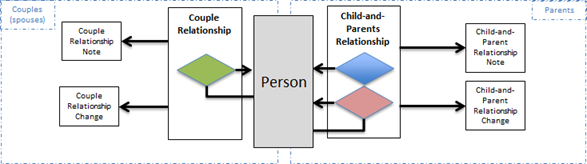
\includegraphics{05/04_relationshipsCore}
        \centering
        \caption{El bloc de l'arbre familiar relatiu a les relacions}\label{img:relationshipsBloc}
    \end{figure}

    Podreu observar també, a les taules que representen l'estructura dels recursos, que a vegades, per la columna que marca el format de dades d'un paràmetre, aquest es troba especificat entre els caràcters `[' i `]'. Aquesta terminologia s'utilitza per indicar que aquest paràmetre és en realitat un recurs o objecte de dades diferent inclòs dins del recurs estudiat.

    També s'observarà que sovint, els recursos exposats, hereten dades d'altres recursos i en els casos que aquests siguin rellevants, se n'exposarà l'estructura a l'apartat `Altres recursos interessants', més endavant en la memòria.

    \subsection{El recurs Relació (Relationship)}

    \paragraph{}
    Aquest recurs s'utilitza en l'actualitat per representar només les relacions de parella. En el passat, també va ser utilitzat per representar relacions entre pares i fills, mitjançant l'ús del paràmetre \emph{type} i l'enumeració \emph{relationshipType}. Tanmateix, aquest ha caigut en el desús des de la incorporació del recurs Relacions Pares i Fill.

    Aquest recurs emmagatzema informació sobre les persones que conformen la relació i els esdeveniments relacionats a aquesta. Les dades pròpies del recurs es mostren a la taula~\ref{res:relationship} i també hereta les dels recursos Subjecte, Conclusió, Enllaços Hypermedia i Dades Extensibles que poden ser trobats a l'apartat `Altres recursos interessants'.

    \begin{center}
             \csvreader[
                separator=comma,
                before table=\sffamily\small,
                longtable={p{2cm-2\tabcolsep}p{3.5cm-2\tabcolsep}p{8.5cm-2\tabcolsep}},
                table head={\caption{Paràmetres del recurs Relació}\label{res:relationship}\\\toprule%
                    \headentry{m{2cm-2\tabcolsep}}{Paràmetre}
                    & \headentry{m{3.4cm-2\tabcolsep}}{Format de Dades}
                    & \headentry{m{8.5cm-2\tabcolsep}}{Descripció}\\\midrule},
                late after line=\\\midrule,
                late after last line=\\\bottomrule,
             ]
             {./tables/05/02_relationships/relation.csv}
             {param=\param,format=\format,desc=\desc}
             {\param&\format&\desc}
     \end{center}


    \subsubsection{L'enumeració relationshipType}

    \paragraph{}
    L'enumeració relationshipType segueix l'estructura de definició GEDCOMX. Com a tal, els valors possibles per l'enumeració segueixen la pauta:\\\verb|http://gedcomx.org/ + `relationshipType'|

    La següent taula mostra els possibles valors per l'enumeració relationshipType, però com ja hem comentat, l'ús del valor ParentChild, ja no s'utilitza en favor del nou recurs Relació Pares i Fill.

    \begin{center}
        \csvreader[
           no head,
           separator=comma,
           table head={\caption{Valors possibles per l'enumeració relationshipType}\label{rel:relationshipType}},
           before table=\sffamily\small,
           longtable={|p{3cm}|p{3cm}|},
           column count=4,
           late after head=\\\hline,
           late after line=\\\hline,
           late after last line=\\\hline,
        ]
        {./tables/05/02_relationships/relationshipType.csv}
        {1=\one,2=\two}
        {\one&\two}
    \end{center}

    \subsection{El recurs Relació Pares i Fill (ChildAndParentsRelationship)}

    \paragraph{}
    Com ja hem comentat, aquest recurs s'utilitza per representar les relacions entre dos pares i un fill. Existeix també la possibilitat de deixar un pare sense especificar, permetent així, la introducció de famílies monoparentals en el sistema.

    Aquest recurs conté informació sobre les persones que conformen els rols de pare, mare i fill, així com el conjunt d'esdeveniments relacionats amb el pare i la mare.

    Els paràmetres del recurs són descrits sa la taula~\ref{res:childAndParents} i recordar que també hereta els paràmetres dels recursos Subjecte, Conclusió, Enllaços Hypermedia i Dades Extensibles que poden ser trobats a l'apartat `Altres recursos interessants'.

    \begin{center}
             \csvreader[
                separator=comma,
                before table=\sffamily\small,
                longtable={p{2cm-2\tabcolsep}p{3.5cm-2\tabcolsep}p{8.5cm-2\tabcolsep}},
                table head={\caption{Paràmetres del recurs Relació Pares i Fill}\label{res:childAndParents}\\\toprule%
                    \headentry{m{2cm-2\tabcolsep}}{Paràmetre}
                    & \headentry{m{3.4cm-2\tabcolsep}}{Format de Dades}
                    & \headentry{m{8.5cm-2\tabcolsep}}{Descripció}\\\midrule},
                late after line=\\\midrule,
                late after last line=\\\bottomrule,
             ]
             {./tables/05/02_relationships/parents.csv}
             {param=\param,format=\format,desc=\desc}
             {\param&\format&\desc}
     \end{center}


    \section{Recursos principals del bloc Discussions}

    \paragraph{}
    El recurs principal d'aquest bloc de l'arbre familiar rep el nom de Discussió, que es troba principalment composta, per comentaris creats mitjançant el recurs Comentari.

    Les discussions a FamilySearch són tòpics de discussió introduïts pels usuaris i relacionades a una persona en concret. Aquestes discussions estan formades per diferents comentaris i destaca la utilització d'un recurs intermedi per fer de pont entre les discussions i els recursos de les persones les quals fan referència accessible a través dels enllaços hypermedia.

    El contingut d'aquestes discussions és divers, però generalment són utilitzades per discutir entre diferents usuaris sobre les dades relatives a una persona, l'origen de les fonts de dades i similars.

    La figura~\ref{img:discussionsBloc} mostra com es troben relacionats els recursos que conformen el bloc Discussions.

    \begin{figure}[h]
        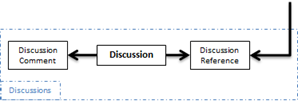
\includegraphics{05/05_discussionsCore}
        \centering
        \caption{El bloc de l'arbre familiar relatiu a les discussions}\label{img:discussionsBloc}
    \end{figure}

    Podreu observar també, a les taules que representen l'estructura dels recursos, que a vegades, per la columna que marca el format de dades d'un paràmetre, aquest es troba especificat entre els caràcters `[' i `]'. Aquesta terminologia s'utilitza per indicar que aquest paràmetre és en realitat un recurs o objecte de dades diferent inclòs dins del recurs estudiat.

    També s'observarà que sovint, els recursos exposats, hereten dades d'altres recursos i en els casos que aquests siguin rellevants, se n'exposarà l'estructura a l'apartat `Altres recursos interessants', més endavant en la memòria.

    \subsection{El recurs Referència a la Discussió (DiscussionsReference)}

    \paragraph{}
    Aquest recurs s'utilitza principalment perquè el recurs Persona puguin accedir al conjunt de discussions que tracten sobre ella i viceversa. En concret, existirà un enllaç per cada una de les discussions que reverenciïn a la mateixa persona.

    Les dades contingudes per aquest recurs poden ser trobades a la taula~\ref{res:discussionReference} i també hereta els paràmetres dels recursos Enllaços Hypermedia i Dades Extensibles que poden ser trobats a l'apartat `Altres recursos interessants'.

    \begin{center}
             \csvreader[
                separator=comma,
                before table=\sffamily\small,
                longtable={p{2cm-2\tabcolsep}p{3.5cm-2\tabcolsep}p{8.5cm-2\tabcolsep}},
                table head={\caption{Paràmetres del recurs Referència a la Discussió}\label{res:discussionReference}\\\toprule%
                    \headentry{m{2cm-2\tabcolsep}}{Paràmetre}
                    & \headentry{m{3.4cm-2\tabcolsep}}{Format de Dades}
                    & \headentry{m{8.5cm-2\tabcolsep}}{Descripció}\\\midrule},
                late after line=\\\midrule,
                late after last line=\\\bottomrule,
             ]
             {./tables/05/03_discussions/discussionReference.csv}
             {param=\param,format=\format,desc=\desc}
             {\param&\format&\desc}
     \end{center}

    \subsection{El recurs Discussió (Discussion)}

    \paragraph{}
    El recurs Discussió és utilitzat per representar el tòpic sobre el qual tractarà la conversació entre els diferents usuaris de FamilySearch i emmagatzemar el conjunt de comentaris introduïts per aquests.

    El recurs Discussió, esdevé un objecte bastant simple, contenint només la informació necessària perquè altres usuaris puguin comprendre el tòpic de discussió, les metadades de la creació i accedir al conjunt de comentaris.

    Aquest recurs està format pels paràmetres mostrats a la taula~\ref{res:discussion} i també hereta els paràmetres dels recursos Enllaços Hypermedia i Dades Extensibles que poden ser trobats a l'apartat `Altres recursos interessants'.

    \clearpage

    \begin{center}
             \csvreader[
                separator=comma,
                before table=\sffamily\small,
                longtable={p{2cm-2\tabcolsep}p{3.5cm-2\tabcolsep}p{8.5cm-2\tabcolsep}},
                table head={\caption{Paràmetres del recurs Discussió}\label{res:discussion}\\\toprule%
                    \headentry{m{2cm-2\tabcolsep}}{Paràmetre}
                    & \headentry{m{3.4cm-2\tabcolsep}}{Format de Dades}
                    & \headentry{m{8.5cm-2\tabcolsep}}{Descripció}\\\midrule},
                late after line=\\\midrule,
                late after last line=\\\bottomrule,
             ]
             {./tables/05/03_discussions/discussion.csv}
             {param=\param,format=\format,desc=\desc}
             {\param&\format&\desc}
     \end{center}

    \subsection{El recurs Comentari (Comment)}

    \paragraph{}
    El recurs Comentari conté els missatges introduïts pels diferents usuaris com a resposta a una discussió. Principalment, conté informació sobre la data de creació, l'usuari que l'ha enviat i el text en qüestió propi del comentari.

    Les dades pròpies d'aquest recurs es mostren a la taula~\ref{res:comment} i també hereta els paràmetres dels recursos Enllaços Hypermedia i Dades Extensibles que poden ser trobats a l'apartat `Altres recursos interessants'.

    \begin{center}
             \csvreader[
                separator=comma,
                before table=\sffamily\small,
                longtable={p{2cm-2\tabcolsep}p{3.5cm-2\tabcolsep}p{8.5cm-2\tabcolsep}},
                table head={\caption{Paràmetres del recurs Comentari}\label{res:comment}\\\toprule%
                    \headentry{m{2cm-2\tabcolsep}}{Paràmetre}
                    & \headentry{m{3.4cm-2\tabcolsep}}{Format de Dades}
                    & \headentry{m{8.5cm-2\tabcolsep}}{Descripció}\\\midrule},
                late after line=\\\midrule,
                late after last line=\\\bottomrule,
             ]
             {./tables/05/03_discussions/comment.csv}
             {param=\param,format=\format,desc=\desc}
             {\param&\format&\desc}
     \end{center}


    \section{Recursos principals del bloc Memòries}

    \paragraph{}
    El bloc Memòries és relativament nou a l'API de FamilySearch i la documentació al respecte és pràcticament inexistent. Aquest bloc conté les memòries penjades al núvol pels usuaris i són relacionades amb les persones de l'arbre familiar.

    Recordem, que el concepte memòries ha estat descrit a la secció tres de la memòria, `L'organització Familysearch' i consisteixen principalment en contingut fotogràfic, històries, documents diversos i fitxers d'àudio.

    El recurs principal d'aquest bloc és el recurs Memòria, que conté tota la informació específica d'aquesta. Les memòries també contenen comentaris, en un estil molt similar a les discussions i també disposen de recursos intermedis per relacionar les memòries amb les persones a les quals fan referència. Com sempre, moltes d'aquestes connexions són implementades a través d'enllaços hypermedia.

    De moment, resulta necessari crear una instància del recurs Memòria per cada contingut que es vulgui pujar al sistema, però la possibilitat de suportar més d'un artefacte amb el mateix recurs memòria ha estat estudiat i en algun moment o altre serà implementat. Un exemple  de cas d'ús podria ser la necessitat de pujar les dues cares d'una fotografia.

    La imatge~\ref{img:memoriesBloc} ofereix un esquema de forma visual de com es relacionen els recursos vinculats al bloc Memòries.

    \begin{figure}[h]
        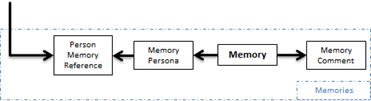
\includegraphics{05/06_memoriesCore}
        \centering
        \caption{El bloc de l'arbre familiar relatiu a les memòries}\label{img:memoriesBloc}
    \end{figure}

    Desgraciadament, la documentació referent a aquest apartat per part de FamilySearch és molt pobre i el contingut de cada un dels recursos ha estat creat per inferència mitjançant el collage de petites peces d'informació i les similituds que presentaven amb altres recursos similars de l'API. És possible que els recursos presentats a continuació no descriguin amb total precisió la realitat exacta.

    Podreu observar també, a les taules que representen l'estructura dels recursos, que a vegades, per la columna que marca el format de dades d'un paràmetre, aquest es troba especificat entre els caràcters `[' i `]'. Aquesta terminologia s'utilitza per indicar que aquest paràmetre és en realitat un recurs o objecte de dades diferent inclòs dins del recurs estudiat.

    També s'observarà que sovint, els recursos exposats, hereten dades d'altres recursos i en els casos que aquests siguin rellevants, se n'exposarà l'estructura a l'apartat `Altres recursos interessants', més endavant en la memòria.

    \subsection{El recurs Referència a la Memòria d'una Persona (Person Memory Reference)}

    \paragraph{}
    Aquest recurs és utilitzat com a pont entre el recurs Persona i el contingut específic de les memòries. Existirà un enllaç hypermedia diferent per cada una de les memòries a les quals el recurs Persona hagi de tenir accés i viceversa.

    Les dades contingudes per aquest recurs poder ser trobades a la taula~\ref{res:memoryReference} i també hereta els paràmetres dels recursos Enllaços Hypermedia i Dades Extensibles que poden ser trobats a l'apartat `Altres recursos interessants'.

    \begin{center}
             \csvreader[
                separator=comma,
                before table=\sffamily\small,
                longtable={p{2cm-2\tabcolsep}p{3.5cm-2\tabcolsep}p{8.5cm-2\tabcolsep}},
                table head={\caption{Paràmetres del recurs Referència a la Memòria d'una Persona}\label{res:memoryReference}\\\toprule%
                    \headentry{m{2cm-2\tabcolsep}}{Paràmetre}
                    & \headentry{m{3.4cm-2\tabcolsep}}{Format de Dades}
                    & \headentry{m{8.5cm-2\tabcolsep}}{Descripció}\\\midrule},
                late after line=\\\midrule,
                late after last line=\\\bottomrule,
             ]
             {./tables/05/04_memories/memoryReference.csv}
             {param=\param,format=\format,desc=\desc}
             {\param&\format&\desc}
     \end{center}

    \subsection{El recurs Persones en una Memòria (MemoryPersona)}

    \paragraph{}
    Aquest recurs s'utilitza com a pont per accedir a totes les persones que han estat marcades com a relacionades en una memòria. Per exemple, si una fotografia conté la imatge de diverses persones i es vol relacionar la memòria amb totes elles, aquest recurs ho fa possible sense la necessitat d'haver de pujar la imatge per cada usuari.

    La taula~\ref{res:memoryPersona} mostra els paràmetres d'aquest recurs que també hereta els paràmetres dels recursos Enllaços Hypermedia i Dades Extensibles que poden ser trobats a l'apartat `Altres recursos interessants'.

    \begin{center}
             \csvreader[
                separator=comma,
                before table=\sffamily\small,
                longtable={p{2cm-2\tabcolsep}p{3.5cm-2\tabcolsep}p{8.5cm-2\tabcolsep}},
                table head={\caption{Paràmetres del recurs Persones en una memòria}\label{res:memoryPersona}\\\toprule%
                    \headentry{m{2cm-2\tabcolsep}}{Paràmetre}
                    & \headentry{m{3.4cm-2\tabcolsep}}{Format de Dades}
                    & \headentry{m{8.5cm-2\tabcolsep}}{Descripció}\\\midrule},
                late after line=\\\midrule,
                late after last line=\\\bottomrule,
             ]
             {./tables/05/04_memories/memoryPersona.csv}
             {param=\param,format=\format,desc=\desc}
             {\param&\format&\desc}
     \end{center}

    \subsection{El recurs Memòria (Memory)}

    \paragraph{}
    El recurs Memòria, com el seu nom indica, és el recurs principal utilitzat per emmagatzemar la informació relacionada amb un artefacte pujat per un usuari. Per fer-ho, s'utilitza el recurs Descripció de la Font de Dades, que s'especificarà més endavant a l'apartat de recursos relacionats amb el bloc de Fonts de Dades.

    Aquest recurs també inclou instàncies dels comentaris que han estat associats a les memòries.

    Els paràmetres d'aquest recurs es mostren a la taula~\ref{res:memory} i també hereta els paràmetres dels recursos Enllaços Hypermedia i Dades Extensibles que poden ser trobats a l'apartat `Altres recursos interessants'.

    \begin{center}
             \csvreader[
                separator=comma,
                before table=\sffamily\small,
                longtable={p{2cm-2\tabcolsep}p{3.5cm-2\tabcolsep}p{8.5cm-2\tabcolsep}},
                table head={\caption{Paràmetres del recurs Memòria}\label{res:memory}\\\toprule%
                    \headentry{m{2cm-2\tabcolsep}}{Paràmetre}
                    & \headentry{m{3.4cm-2\tabcolsep}}{Format de Dades}
                    & \headentry{m{8.5cm-2\tabcolsep}}{Descripció}\\\midrule},
                late after line=\\\midrule,
                late after last line=\\\bottomrule,
             ]
             {./tables/05/04_memories/memory.csv}
             {param=\param,format=\format,desc=\desc}
             {\param&\format&\desc}
     \end{center}


    \section{Recursos principals del bloc Fonts de Dades}

    \paragraph{}
    Aquest bloc de l'arbre familiar destaca pels recursos Col·lecció i Font de Dades, que s'utilitzen per certificar la veracitat de les dades referents a les persones que es poden trobar a l'arbre familiar o les relacions que les uneixen.

    Aquest bloc és realment important, ja que és l'encarregat de garantir la integritat de les dades i per tant, d'assegurar que la informació continguda a l'arbre familiar de FamilySearch sigui usable i interessant pels usuaris de l'aplicació.

    Així doncs, les fonts de dades són utilitzades per demostrar que un esdeveniment en concret va succeir o que les dades de la persona citada són les mateixes que aquelles redactades en els documents oficials.

    Les fonts de dades s'agrupen i emmagatzemen en col·leccions i cada persona o relació, disposa d'un recurs que actua com intermediari per relacionar-los amb les fonts de dades. Com sempre, els enllaços explícits entre els diferents recursos es realitzen mitjançant els enllaços hypermedia. La imatge~\ref{img:sourcesBloc} ofereix una vista de com s'estructuren i relacionen els diferents recursos del bloc Font de Dades.

    \begin{figure}[h]
        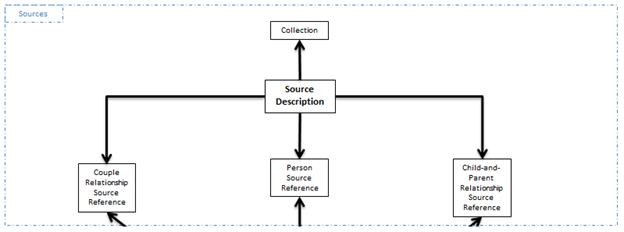
\includegraphics{05/07_sourcesCore}
        \centering
        \caption{El bloc de l'arbre familiar relatiu a les fonts de dades}\label{img:sourcesBloc}
    \end{figure}

    Podreu observar també, a les taules que representen l'estructura dels recursos, que a vegades, per la columna que marca el format de dades d'un paràmetre, aquest es troba especificat entre els caràcters `[' i `]'. Aquesta terminologia s'utilitza per indicar que aquest paràmetre és en realitat un recurs o objecte de dades diferent inclòs dins del recurs estudiat.

    També s'observarà que sovint, els recursos exposats, hereten dades d'altres recursos i en els casos que aquests siguin rellevants, se n'exposarà l'estructura a l'apartat `Altres recursos interessants', més endavant en la memòria.

    \subsection{El recurs Col·lecció (Collection)}

    \paragraph{}
    Aquest recurs representa una col·lecció o agregació, de fonts de dades de caràcter genealògic.

    Aquestes dades poden fer referència tant a les dades internes de FamilySearch, com als registres bolcats per tercers a les bases de dades. Per tal d'ajudar al lector a fer-se una idea, una col·lecció podria ser per exemple el conjunt de fonts de dades que conformen l'arbre familiar.

    La taula~\ref{res:collection} mostra els paràmetres que aquest recurs incorpora i també hereta els paràmetres dels recursos Enllaços Hypermedia i Dades Extensibles que poden ser trobats a l'apartat `Altres recursos interessants'.

    \begin{center}
             \csvreader[
                separator=comma,
                before table=\sffamily\small,
                longtable={p{2cm-2\tabcolsep}p{3.5cm-2\tabcolsep}p{8.5cm-2\tabcolsep}},
                table head={\caption{Paràmetres del recurs Col·lecció}\label{res:collection}\\\toprule%
                    \headentry{m{2cm-2\tabcolsep}}{Paràmetre}
                    & \headentry{m{3.4cm-2\tabcolsep}}{Format de Dades}
                    & \headentry{m{8.5cm-2\tabcolsep}}{Descripció}\\\midrule},
                late after line=\\\midrule,
                late after last line=\\\bottomrule,
             ]
             {./tables/05/05_sources/collection.csv}
             {param=\param,format=\format,desc=\desc}
             {\param&\format&\desc}
     \end{center}

    \subsection{El recurs Contingut de la Col·lecció (CollectionContent)}

    \paragraph{}
    Aquest recurs conté informació específica sobre la col·lecció a la que fa referència. Serveix per  comprendre millor l'estat actual de migració de la col·lecció a les bases de dades de FamilySearch, així com informació sobre el contingut que aquesta aporta.

    La taula~\ref{res:collectionContent} mostra els paràmetres inclosos en el recurs, que a la vegada hereta els paràmetres dels recursos Enllaços Hypermedia i Dades Extensibles que poden ser trobats a l'apartat `Altres recursos interessants'.

    \begin{center}
             \csvreader[
                separator=comma,
                before table=\sffamily\small,
                longtable={p{2cm-2\tabcolsep}p{3.5cm-2\tabcolsep}p{8.5cm-2\tabcolsep}},
                table head={\caption{Paràmetres del recurs Contingut de la Col·lecció}\label{res:collectionContent}\\\toprule%
                    \headentry{m{2cm-2\tabcolsep}}{Paràmetre}
                    & \headentry{m{3.4cm-2\tabcolsep}}{Format de Dades}
                    & \headentry{m{8.5cm-2\tabcolsep}}{Descripció}\\\midrule},
                late after line=\\\midrule,
                late after last line=\\\bottomrule,
             ]
             {./tables/05/05_sources/collectionContent.csv}
             {param=\param,format=\format,desc=\desc}
             {\param&\format&\desc}
     \end{center}

    \subsection{El recurs Atribució (Attribution)}

    \paragraph{}
    El recurs Atribució s'utilitza en més llocs que les fonts de dades, però com que juga un paper especialment important en aquest, hem decidit incloure'l dins d'aquesta secció.

    Aquest recurs conté principalment paràmetres que permeten descriure qui, quan i perquè, va ser realitzada una contribució o modificació sobre les dades.

    Els paràmetres d'aquest recurs són descrits a la taula~\ref{res:attribution}, que també hereta els paràmetres del recurs Dades Extensibles que pot ser trobat a l'apartat `Altres recursos interessants'.

    \begin{center}
             \csvreader[
                separator=comma,
                before table=\sffamily\small,
                longtable={p{2cm-2\tabcolsep}p{3.5cm-2\tabcolsep}p{8.5cm-2\tabcolsep}},
                table head={\caption{Paràmetres del recurs Atribució}\label{res:attribution}\\\toprule%
                    \headentry{m{2cm-2\tabcolsep}}{Paràmetre}
                    & \headentry{m{3.4cm-2\tabcolsep}}{Format de Dades}
                    & \headentry{m{8.5cm-2\tabcolsep}}{Descripció}\\\midrule},
                late after line=\\\midrule,
                late after last line=\\\bottomrule,
             ]
             {./tables/05/05_sources/attribution.csv}
             {param=\param,format=\format,desc=\desc}
             {\param&\format&\desc}
     \end{center}

    \subsection{El recurs Font de Dades (SourceDescription)}

    \paragraph{}
    Aquest recurs defineix una font de dades i n'emmagatzema tota la informació que la caracteritza. Les fonts de dades formen part d'una col·lecció i es troben relacionades a ella mitjançant enllaços hypermedia.

    La millor forma d'explicar aquest recurs és comprendre'n els paràmetres i aquests s'exposen a la taula~\ref{res:sourceDescription}. El recurs Font de Dades també hereta els paràmetres dels recursos Enllaços Hypermedia i Dades Extensibles que poden ser trobats a l'apartat `Altres recursos interessants'.

    \begin{center}
             \csvreader[
                separator=comma,
                before table=\sffamily\small,
                longtable={p{2cm-2\tabcolsep}p{3.5cm-2\tabcolsep}p{8.5cm-2\tabcolsep}},
                table head={\caption{Paràmetres del recurs Font de Dades}\label{res:sourceDescription}\\\toprule%
                    \headentry{m{2cm-2\tabcolsep}}{Paràmetre}
                    & \headentry{m{3.4cm-2\tabcolsep}}{Format de Dades}
                    & \headentry{m{8.5cm-2\tabcolsep}}{Descripció}\\\midrule},
                late after line=\\\midrule,
                late after last line=\\\bottomrule,
             ]
             {./tables/05/05_sources/sourceDescription.csv}
             {param=\param,format=\format,desc=\desc}
             {\param&\format&\desc}
     \end{center}


    \subsubsection{L'enumeració resourceType}

    L'enumeració resourceType segueix l'estructura de definició GEDCOMX. Com a tal, els valors possibles per l'enumeració segueixen la pauta:\\\verb|http://gedcomx.org/ + `resourceType'|

    La següent taula mostra els possibles valors per l'enumeració resourceType.

    \begin{center}
        \csvreader[
           no head,
           separator=comma,
           table head={\caption{Valors possibles per l'enumeració resourceType}\label{enum:resourceType}},
           before table=\sffamily\small,
           longtable={|p{3cm}|p{3cm}|p{3cm}|},
           column count=3,
           late after head=\\\hline,
           late after line=\\\hline,
           late after last line=\\\hline,
        ]
        {./tables/05/05_sources/resourceType.csv}
        {1=\one,2=\two,3=\three}
        {\one&\two&\three}
    \end{center}

    \subsection{El recurs Referència a la Font de Dades (SourceReference)}

    \paragraph{}
    Aquest recurs s'utilitza per fer de pont entre els diferents recursos de l'arbre familiar que contenen informació genealògica i les fonts de dades que l'han proporcionat.

    Com s'ha pogut veure en la imatge [ref] que obria el bloc de Fonts de Dades, el recurs Referència a la Font de Dades aplica tant a les relacions familiars com a les persones. De la mateixa forma, també es veu utilitzat aquest recurs per referenciar unes Fonts de Dades, amb algunes altres.

    A part dels paràmetres que conformen aquest recurs i que es mostren a la taula~\ref{res:sourceReference}, també hereta els paràmetres dels recursos Enllaços Hypermedia i Dades Extensibles que poden ser trobats a l'apartat `Altres recursos interessants'.

    \begin{center}
             \csvreader[
                separator=comma,
                before table=\sffamily\small,
                longtable={p{2cm-2\tabcolsep}p{3.5cm-2\tabcolsep}p{8.5cm-2\tabcolsep}},
                table head={\caption{Recurs Referència a la Font de Dades}\label{res:sourceReference}\\\toprule%
                    \headentry{m{2cm-2\tabcolsep}}{Paràmetre}
                    & \headentry{m{3.4cm-2\tabcolsep}}{Format de Dades}
                    & \headentry{m{8.5cm-2\tabcolsep}}{Descripció}\\\midrule},
                late after line=\\\midrule,
                late after last line=\\\bottomrule,
             ]
             {./tables/05/05_sources/sourceReference.csv}
             {param=\param,format=\format,desc=\desc}
             {\param&\format&\desc}
     \end{center}


    \section{Altres recursos interessants}

    \paragraph{}
    Com haureu pogut observar després de la lectura de les seccions anteriors, no tots els objectes o recursos que han anat apareixent com a paràmetres dels diferents recursos estudiants, han estat descrits en profunditat. Les raons són diverses segons el recurs en qüestió, però alguns motius comuns són els següents:

    \begin{itemize}
        \item És un recurs orientat a la manipulació de les dades més que a proporcionar informació genealògica a l'usuari i per tant, no acaba de prendre valor per l'estudi realitzat en els apartats anteriors.
        \item Es tracta d'un recurs simple del qual no s'aportaria més informació mostrant-ne l'estructura, que simplement disposant de la descripció del camp.
        \item És un recurs utilitzat en cassos molt específics i per tant, no aplicable en un àmbit general.
    \end{itemize}

    Això no obstant, sí que hi ha altres recursos que s'han vist representats a les seccions anteriors de forma transversal, com per exemple en les imatges que unien els diferents recursos d'un bloc, i que volem explicar. Exemples d'aquests recursos són les notes i els històrics de canvis.

    També existeix un conjunt de recursos que hem anat mencionant en els apartats anteriors, on els recursos estudiats, heretaven els paràmetres d'aquests. Aquests recursos incorporats de forma global a molts altres, també seran estudiats en aquest apartat de la memòria.

    A part d'aquests dos grups de recursos, també volem descriure'n d'altres que considerem que sota certes circumstàncies podrien resultar interessants i encara que no s'han vist relacionats de forma directa amb els blocs de dades anteriors, volem deixar-ne constància en el projecte.

    \subsection{El recurs Subjecte (Subject)}

    \paragraph{}
    El recurs Subjecte fa referència al concepte abstracte de subjecte genealògic, entenent-lo com una entitat única que o bé pot fer referència a una persona o a una localització concreta sobre el globus terraqüi.

    Aquesta entitat única, agrega i emmagatzema les diferents evidències i fonts de dades particulars del subjecte, és a dir, el col·lectiu d'informació que fan que aquest subjecte sigui diferent dels altres.

    La taula~\ref{res:subject} mostra al que ens referim quan parlem d'aquesta agregació d'informació.

    \begin{center}
             \csvreader[
                separator=comma,
                before table=\sffamily\small,
                longtable={p{2cm-2\tabcolsep}p{3.5cm-2\tabcolsep}p{8.5cm-2\tabcolsep}},
                table head={\caption{Paràmetres del recurs Subjecte}\label{res:subject}\\\toprule%
                    \headentry{m{2cm-2\tabcolsep}}{Paràmetre}
                    & \headentry{m{3.4cm-2\tabcolsep}}{Format de Dades}
                    & \headentry{m{8.5cm-2\tabcolsep}}{Descripció}\\\midrule},
                late after line=\\\midrule,
                late after last line=\\\bottomrule,
             ]
             {./tables/05/06_others/subject.csv}
             {param=\param,format=\format,desc=\desc}
             {\param&\format&\desc}
     \end{center}

    \subsection{El recurs Conclusió (Conclusion)}

    \paragraph{}
    En l'àmbit de l'API de FamilySearch, el terme conclusió fa referència al valor que pren una dada genealògica després de ser contrastada amb una font de dades. És doncs, l'avaluació del valor que certa dada genealògica, o conjunt de dades genealògiques, han rebut.

    Aquest recurs conté els paràmetres que s'expressen a la taula~\ref{res:conclusion}:

    \begin{center}
             \csvreader[
                separator=comma,
                before table=\sffamily\small,
                longtable={p{2cm-2\tabcolsep}p{3.5cm-2\tabcolsep}p{8.5cm-2\tabcolsep}},
                table head={\caption{Paràmetres del recurs Conclusió}\label{res:conclusion}\\\toprule%
                    \headentry{m{2cm-2\tabcolsep}}{Paràmetre}
                    & \headentry{m{3.4cm-2\tabcolsep}}{Format de Dades}
                    & \headentry{m{8.5cm-2\tabcolsep}}{Descripció}\\\midrule},
                late after line=\\\midrule,
                late after last line=\\\bottomrule,
             ]
             {./tables/05/06_others/conclusion.csv}
             {param=\param,format=\format,desc=\desc}
             {\param&\format&\desc}
     \end{center}

    \subsection{El recurs Enllaços Hypermedia (Hypermedia Enabled Data)}

    \paragraph{}
    Aquest recurs es troba en pràcticament tots els altres recursos de l'API de FamilySearch. Són els responsables de poder navegar, a través dels diferents recursos que es troben enllaçats en el model de dades de FamilySearch, sense necessitat de codificar noves URIs de forma manual, o des d'una aplicació.

    Aquest recurs consisteix bàsicament en un conjunt d'enllaços que apunten als diferents recursos. La taula~\ref{res:hypermedia} en mostra l'estructura en detall.

    \begin{center}
             \csvreader[
                separator=comma,
                before table=\sffamily\small,
                longtable={p{2cm-2\tabcolsep}p{3.5cm-2\tabcolsep}p{8.5cm-2\tabcolsep}},
                table head={\caption{Paràmetres del recurs Enllaços Hypermedia}\label{res:hypermedia}\\\toprule%
                    \headentry{m{2cm-2\tabcolsep}}{Paràmetre}
                    & \headentry{m{3.4cm-2\tabcolsep}}{Format de Dades}
                    & \headentry{m{8.5cm-2\tabcolsep}}{Descripció}\\\midrule},
                late after line=\\\midrule,
                late after last line=\\\bottomrule,
             ]
             {./tables/05/06_others/hypermedia.csv}
             {param=\param,format=\format,desc=\desc}
             {\param&\format&\desc}
     \end{center}

    \subsection{El recurs Enllaç (Link)}

    \paragraph{}
    A diferència del que es pugui creure, en el context de l'API de FamilySearch, Link no fa referència al famós protagonista de la saga de videojocs `Zelda', sinó a un enllaç hypermedia com el descrit en els començaments d'aquesta secció de la memòria.

    Com ja s'ha comentat nombroses vegades, aquests enllaços existeixen per facilitar la navegació entre recursos. L'estructura del recurs Enllaç pot veure's en detall a la taula~\ref{res:link}.

    \begin{center}
             \csvreader[
                separator=comma,
                before table=\sffamily\small,
                longtable={p{2cm-2\tabcolsep}p{3.5cm-2\tabcolsep}p{8.5cm-2\tabcolsep}},
                table head={\caption{Paràmetres del recurs Enllaç}\label{res:link}\\\toprule%
                    \headentry{m{2cm-2\tabcolsep}}{Paràmetre}
                    & \headentry{m{3.4cm-2\tabcolsep}}{Format de Dades}
                    & \headentry{m{8.5cm-2\tabcolsep}}{Descripció}\\\midrule},
                late after line=\\\midrule,
                late after last line=\\\bottomrule,
             ]
             {./tables/05/06_others/link.csv}
             {param=\param,format=\format,desc=\desc}
             {\param&\format&\desc}
     \end{center}

    \subsection{El recurs Dades Extensibles (Extensible Data)}

    \paragraph{}
    Aquest recurs és probablement el més simple de tots. S'encarrega de dotar a tots els altres recursos de l'API de FamilySearch, amb un identificador local únic que permeti referenciar-lo a les bases de dades.

    La taula~\ref{res:extensibleData} mostra l'estructura d'aquest recurs.

    \begin{center}
             \csvreader[
                separator=comma,
                before table=\sffamily\small,
                longtable={p{2cm-2\tabcolsep}p{3.5cm-2\tabcolsep}p{8.5cm-2\tabcolsep}},
                table head={\caption{Paràmetres del recurs Dades Extensibles}\label{res:extensibleData}\\\toprule%
                    \headentry{m{2cm-2\tabcolsep}}{Paràmetre}
                    & \headentry{m{3.4cm-2\tabcolsep}}{Format de Dades}
                    & \headentry{m{8.5cm-2\tabcolsep}}{Descripció}\\\midrule},
                late after line=\\\midrule,
                late after last line=\\\bottomrule,
             ]
             {./tables/05/06_others/extensibleData.csv}
             {param=\param,format=\format,desc=\desc}
             {\param&\format&\desc}
     \end{center}

    \subsection{El recurs Nota (Note)}

    \paragraph{}
    Aquest recurs pot ser vinculat a persones, relacions i fonts de dades. És un recurs utilitzat per realitzar alguna anotació específica sobre les dades a les quals ha estat relacionat.

    El recurs Nota, també hereta els paràmetres dels recursos Enllaços Hypermedia i Dades Extensibles, que poden trobar-se en aquest mateix apartat de la memòria i té per paràmetres propis els que es mostren a la taula~\ref{res:note}.

    \begin{center}
             \csvreader[
                separator=comma,
                before table=\sffamily\small,
                longtable={p{2cm-2\tabcolsep}p{3.5cm-2\tabcolsep}p{8.5cm-2\tabcolsep}},
                table head={\caption{Paràmetres del recurs Nota}\label{res:note}\\\toprule%
                    \headentry{m{2cm-2\tabcolsep}}{Paràmetre}
                    & \headentry{m{3.4cm-2\tabcolsep}}{Format de Dades}
                    & \headentry{m{8.5cm-2\tabcolsep}}{Descripció}\\\midrule},
                late after line=\\\midrule,
                late after last line=\\\bottomrule,
             ]
             {./tables/05/06_others/note.csv}
             {param=\param,format=\format,desc=\desc}
             {\param&\format&\desc}
     \end{center}

    \subsection{El recurs Referència al Recurs (ResourceReference)}

    \paragraph{}
    Un altre recurs que ha sortit molt fins ara, com a recurs contingut dins dels altres recursos, és el de Referència al Recurs. Aquest objecte, s'utilitza per enllaçar mitjançant un contingut semàntic, representat per l'identificador del camp del recurs apuntat i la seva URI, un recurs amb un altre.

    El seu format és molt simple i consta només dels dos paràmetres exposats a la taula~\ref{res:resourceReference}.

    \begin{center}
             \csvreader[
                separator=comma,
                before table=\sffamily\small,
                longtable={p{2cm-2\tabcolsep}p{3.5cm-2\tabcolsep}p{8.5cm-2\tabcolsep}},
                table head={\caption{Paràmetres del recurs Referència al Recurs}\label{res:resourceReference}\\\toprule%
                    \headentry{m{2cm-2\tabcolsep}}{Paràmetre}
                    & \headentry{m{3.4cm-2\tabcolsep}}{Format de Dades}
                    & \headentry{m{8.5cm-2\tabcolsep}}{Descripció}\\\midrule},
                late after line=\\\midrule,
                late after last line=\\\bottomrule,
             ]
             {./tables/05/06_others/resourceReference.csv}
             {param=\param,format=\format,desc=\desc}
             {\param&\format&\desc}
     \end{center}

    \subsection{El recurs Usuari (User)}

    \paragraph{}
    El recurs Usuari conté tota la informació relacionada a l'usuari que es troba identificat amb l'aplicació FamilySearch.

    Aquesta informació pot resultar d'interès pels frontals de les aplicacions en cas de desitjar realitzar alguna mena de personalització del contingut o inclòs realitzar temes d'analítica web. També pot ser utilitzada per accedir a l'arbre genealògic de l'usuari o al recurs de la seva persona a l'arbre familiar.

     Aquest recurs, com molts altres que ja hem exposat, també hereta els paràmetres dels recursos Enllaços Hypermedia i Dades Extensibles, que poden trobar-se en aquest mateix apartat de la memòria i té, per paràmetres propis, els que es mostren a la taula~\ref{res:user}.

     \begin{center}
              \csvreader[
                 separator=comma,
                 before table=\sffamily\small,
                 longtable={p{4cm-2\tabcolsep}p{2cm-2\tabcolsep}p{8cm-2\tabcolsep}},
                 table head={\caption{Paràmetres del recurs Usuari}\label{res:user}\\\toprule%
                     \headentry{m{4cm-2\tabcolsep}}{Paràmetre}
                     & \headentry{m{2cm-2\tabcolsep}}{Format de Dades}
                     & \headentry{m{8cm-2\tabcolsep}}{Descripció}\\\midrule},
                 late after line=\\\midrule,
                 late after last line=\\\bottomrule,
              ]
              {./tables/05/06_others/user.csv}
              {param=\param,format=\format,desc=\desc}
              {\param&\format&\desc}
      \end{center}

    \subsection{El recurs Canvi (Change)}

    \paragraph{}
    Un altre recurs transversal, per alguns dels recursos més importants de l'API de FamilySearch, és el recurs Canvi.

    Quan un usuari realitza alguna modificació de qualsevol mena, ja sigui sobre la informació d'una persona o sobre una relació de parella o parental, aquest canvi queda enregistrat per diversos motius.

    El primer, poder veure com les dades s'han anat modificat al llarg del temps i veure'n la progressió. El segon, poder recuperar un estat anterior en cas d'error o problema en el sistema.

    El recurs Canvi està format pels paràmetres mostrats a la taula~\ref{res:change}.

    \begin{center}
             \csvreader[
                separator=comma,
                before table=\sffamily\small,
                longtable={p{2cm-2\tabcolsep}p{3.5cm-2\tabcolsep}p{8.5cm-2\tabcolsep}},
                table head={\caption{Paràmetres del recurs Canvi}\label{res:change}\\\toprule%
                    \headentry{m{2cm-2\tabcolsep}}{Paràmetre}
                    & \headentry{m{3.4cm-2\tabcolsep}}{Format de Dades}
                    & \headentry{m{8.5cm-2\tabcolsep}}{Descripció}\\\midrule},
                late after line=\\\midrule,
                late after last line=\\\bottomrule,
             ]
             {./tables/05/06_others/change.csv}
             {param=\param,format=\format,desc=\desc}
             {\param&\format&\desc}
     \end{center}


     \subsubsection{L'enumeració changeObjectModifier}

     \paragraph{}
     L'enumeració changeObjectModifier segueix l'estructura de definició GEDCOMX. Com a tal, els valors possibles per l'enumeració segueixen la pauta:\\\verb|http://gedcomx.org/ + `changeObjectModifier'|

     La taula~\ref{enum:changeObjectModifier} mostra els possible valors de l'enumeració changeOperation.

     \begin{center}
         \csvreader[
            no head,
            separator=comma,
            table head={\caption{Valors possibles per l'enumeració changeObjectModifier}\label{enum:changeObjectModifier}},
            before table=\sffamily\small,
            longtable={|p{3cm}|p{3cm}|p{6cm}|},
            column count=4,
            late after head=\\\hline,
            late after line=\\\hline,
            late after last line=\\\hline,
         ]
         {./tables/05/06_others/changeObjectModifier.csv}
         {1=\one,2=\two,3=\three}
         {\one&\two&\three}
     \end{center}


     \subsubsection{L'enumeració changeOperation}

     \paragraph{}
     L'enumeració changeOperation segueix l'estructura de definició GEDCOMX. Com a tal, els valors possibles per l'enumeració segueixen la pauta:\\\verb|http://gedcomx.org/ + `changeOperation'|

     La taula~\ref{enum:changeOperation} mostra els possibles valors de l'enumeració changeOperation.

     \begin{center}
         \csvreader[
            no head,
            separator=comma,
            table head={\caption{Valors possibles per l'enumeració changeOperation}\label{enum:changeOperation}},
            before table=\sffamily\small,
            longtable={|p{3cm}|p{3cm}|p{3cm}|p{3cm}|},
            column count=4,
            late after head=\\\hline,
            late after line=\\\hline,
            late after last line=\\\hline,
         ]
         {./tables/05/06_others/changeOperation.csv}
         {1=\one,2=\two,3=\three,4=\four}
         {\one&\two&\three&\four}
     \end{center}


     \subsubsection{L'enumeració changeObjectType}

     \paragraph{}
     L'enumeració changeObjectType segueix l'estructura de definició GEDCOMX. Com a tal, els valors possibles per l'enumeració segueixen la pauta:\\\verb|http://gedcomx.org/ + `changeObjectType'|

     La taula~\ref{enum:changeObjectType} mostra els possibles valors de l'enumeració changeObjectType.

     \begin{center}
         \csvreader[
            no head,
            separator=comma,
            table head={\caption{Valors possibles per l'enumeració changeObjectType}\label{enum:changeObjectType}},
            before table=\sffamily\small,
            longtable={|p{3cm}|p{3cm}|p{3cm}|p{3cm}|},
            column count=4,
            late after head=\\\hline,
            late after line=\\\hline,
            late after last line=\\\hline,
         ]
         {./tables/05/06_others/changeObjectType.csv}
         {1=\one,2=\two,3=\three,4=\four}
         {\one&\two&\three&\four}
     \end{center}

    \subsection{El recurs Agent (Agent)}

    \paragraph{}
    El recurs agent representa a una persona, organització o col·lectiu. En la recerca genealògica, un Agent, generalment pren el rol de contribuïdor.

    La gran majoria dels paràmetres de contribuïdors, que ens hem trobat fins ara en els diferents recursos, apunten a una instància de recurs Agent.

    Aquest recurs conté la informació específica que detallem a la taula~\ref{res:agent} així com els paràmetres heretats dels recursos Enllaços Hypermedia i Dades Extensibles.

    \begin{center}
             \csvreader[
                separator=comma,
                before table=\sffamily\small,
                longtable={p{2cm-2\tabcolsep}p{3.5cm-2\tabcolsep}p{8.5cm-2\tabcolsep}},
                table head={\caption{Paràmetres del recurs Agent}\label{res:agent}\\\toprule%
                    \headentry{m{2cm-2\tabcolsep}}{Paràmetre}
                    & \headentry{m{3.4cm-2\tabcolsep}}{Format de Dades}
                    & \headentry{m{8.5cm-2\tabcolsep}}{Descripció}\\\midrule},
                late after line=\\\midrule,
                late after last line=\\\bottomrule,
             ]
             {./tables/05/06_others/agent.csv}
             {param=\param,format=\format,desc=\desc}
             {\param&\format&\desc}
     \end{center}


    \section{Camins d'accés a l'arbre familiar i operacions de cerca}

    \paragraph{}
    L'accés a les dades contingudes per l'API de FamilySearch es pot realitzar de maneres diferents segons la informació inicial coneguda en el moment d’iniciar la cerca.

    Tot procés de cerca es podria dividir en dues fases principals, on la segona, realment podria ser dividida en diverses opcions diferents. Aquestes dues fases consisteixen en:

    \begin{enumerate}
        \item Accedir al sistema de FamilySearch mitjançant un usuari i contrasenya.
        \item Accedir a les dades de forma directa o indirecta segons la informació coneguda.
    \end{enumerate}

    La imatge~\ref{fig:dataAcessPath} ofereix una vista preliminar de les diferents opcions disponibles per tal d'accedir a les dades de FamilySearch relacionades amb les persones. En els següents apartats, s'exposarà el comportament dels mètodes directes i indirectes d'accés a les dades.

    \begin{figure}[h]
        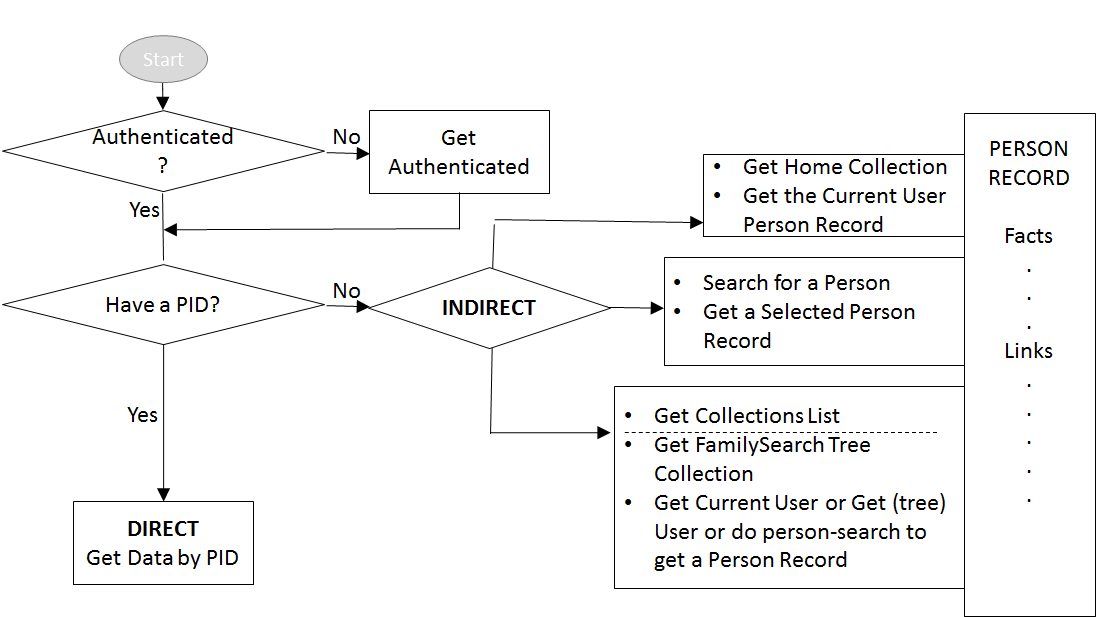
\includegraphics[width=\linewidth]{05/08_dataAccessPaths}
        \centering
        \caption{Sistemes d'accés a les dades de l'arbre familiar}\label{fig:dataAcessPath}
    \end{figure}


    \subsection{L'accés directe a les dades}

        \paragraph{}
        L'accés directe a les dades es pot realitzar si es coneix l'identificador del recurs que vol ser consultat.

        Per exemple, si es coneix el PID de la persona a consultar, es pot codificar des de les aplicacions el diferent conjunt d'URIs per manipular els recursos i evitar així la necessitat de passar pel sistema. D'aquesta forma, es pot doncs accedir a la informació de la persona, memòries, discussions, fills, pares, parelles, avantpassats i descendència; sempre i quan, es conegui tota la informació necessària per codificar les diferents URIs d'accés.

        Un exemple d'ús, podria ser per exemple, donat un identificador de persona conegut, accedir directament a les seves memòries mitjançant la codificació de la URI i evitar, així, haver de passar per l'arbre familiar.


    \subsection{L'accés indirecte a les dades}

        \paragraph{}
        A pesar que poder accedir directament a les dades, pot semblar un procés ideal, el més normal és que ens trobem en la situació de necessitar realitzar un accés indirecte a les dades. En altres paraules, accedir en primera instància als recursos del sistema i obtenir així els diferents enllaços que ens condueixin cap a les operacions desitjades.

        Per descobrir l’URI del recurs exacte que vol ser consultat, existeixen principalment tres opcions diferents:

        \begin{itemize}
            \item Llegir la col·lecció Arrel, que representa la col·lecció que conté totes les dades de FamilySearch i seguir-la per tal d'obtenir l'usuari identificat. Un cop es disposa de la persona relacionada a l'usuari, es pot accedir a qualsevol altre recurs mitjançant els enllaços hypermedia de la resposta i simular, de forma dinàmica, el mateix que podríem haver realitzat mitjançant l'accés directe.
            \item Llegir la llista de col·leccions disponibles per tal d'accedir a l'arbre familiar o accedir a ell de forma directa. Un cop es disposa de l'arbre familiar es pot llegir l'usuari actual o la persona de l'usuari i d'aquí procedir com es desitgi. Una alternativa és accedir mitjançant els enllaços o plantilles URL, als recursos generals de Memòries, Discussions, Relacions, etcètera i consultar la informació general d'aquests recursos mitjançant els seus identificadors retornats.
            \item La tercera opció, i probablement la més comuna, passa per la realització d'una cerca contra la base de dades de FamilySearch per tal d'obtenir una Persona o Localització. Un cop s'obté el resultat de la cerca, es pot navegar a qualsevol de les peces d'informació relacionades als recursos consultats, mitjançant les URI i enllaços hypermedia de les respostes.
        \end{itemize}

        El procés descrit en el tercer punt de les opcions de cerca indirecta, serà el més comú de cara a accedir a la informació, ja que les altres opcions no permeten gaire filtratge de les dades, a menys que coneguem la col·lecció específica sobre la qual volem realitzar una investigació genealògica o només vulguem consultar la informació de l'arbre familiar, de l'usuari identificat.

        Com hem comentat doncs, són quatre les principals opcions d'entrada que permeten obtenir persones concretes de l'arbre de forma indirecta i començar a navegar, des de la resposta d'aquestes, per les dades genealògiques.

        En els següents apartats,  s'explicarà en més detall com poden ser configurades cada una d'aquestes operacions.


    \subsection{Lectura de l'usuari identificat}

        \paragraph{}
        Aquesta operació pot ser realitzada de forma directe, accedint a la URI:

        \begin{displayquote}
            \emph{/platform/users/current}
        \end{displayquote}

        La crida retorna la informació específica del recurs Usuari descrita en els apartats anteriors d'aquesta memòria. Des d'aquest, es pot accedir a la persona de l'arbre familiar que representa a l'usuari i des d’aquesta, a qualsevol altre peça d'informació genealògica relacionada amb la persona.


    \subsection{Lectura de la persona relacionada a l'usuari identificat}

        Aquesta operació és realitzable a través de la URI:

        \begin{displayquote}
            \emph{/platform/tree/current-person}
        \end{displayquote}

        L'operació en qüestió retorna el recurs Persona de l'usuari identificat, amb tota la informació descrita en els apartats anteriors de la memòria. Des d'aquest, es pot navegar a qualsevol altre recurs o dada genealògica relacionada.

        Aquesta forma d'accés representa un pas menys que l’exposada en l’apartat anterior, si sabem d'entrada que volem accedir a l'arbre familiar. En cas que també volguéssim alguna dada del recurs Usuari, caldria entrar per la funcionalitat descrita en l'apartat anterior.


    \subsection{Cerca de Persones a l'arbre familiar}

        \paragraph{}
        L'operació cerca de persones, a l'arbre familiar, és sense cap dubte la més interessant de totes les funcionalitats que ofereix l'API.

        Aquesta operació es realitza mitjançant una petició a la URI /platform/tree/search, que a més a més, pot ser configurada i personalitzada mitjançant la inclusió de diferents paràmetres.

        Un cop finalitzada la petició, aquesta retorna el conjunt de persones de l'arbre familiar, que compleixen amb les condicions imposades en la cerca. L'usuari, pot començar a navegar per la resposta, accedint a aquelles persones que li resultin de més interès i a tots els altres recursos disponibles relacionats amb aquestes.

        Es pot entendre la funcionalitat de cerca a l'arbre familiar, com una porta a totes les dades emmagatzemades per FamilySearch.

        La cerca pot ser controlada mitjançant tres paràmetres principals, un dels quals, accepta molts paràmetres secundaris. Els paràmetres principals són descrits a la taula~\ref{res:searchPersonMain}.

        \begin{center}
                 \csvreader[
                    separator=comma,
                    before table=\sffamily\small,
                    respect tilde=true,
                    respect leftbrace=true,
                    respect rightbrace=true,
                    longtable={p{2cm-2\tabcolsep}p{12cm-2\tabcolsep}},
                    table head={\caption{Variables principals per la cerca de persones}\label{res:searchPersonMain}\\\toprule%
                        \headentry{m{2cm-2\tabcolsep}}{Variable}
                        & \headentry{m{12cm-2\tabcolsep}}{Descripció}\\\midrule},
                    late after line=\\\midrule,
                    late after last line=\\\bottomrule,
                 ]
                 {./tables/05/10_search/searchPersonMain.csv}
                 {var=\var,desc=\desc}
                 {\var&\desc}
         \end{center}

         El paràmetre \emph{q}, descrit en la taula~\ref{res:searchPersonMain}, accepta com a paràmetres vàlids els camps exposats a la taula~\ref{res:searchPersonSec}. L'etiqueta \{relation\}, dels camps d'aquesta taula,  pot ser reemplaçada per qualsevol dels següents valors: father, mother, spouse (pare, mare, parella).

         \begin{center}
                  \csvreader[
                     separator=comma,
                     before table=\sffamily\small,
                     respect tilde=true,
                     respect leftbrace=true,
                     respect rightbrace=true,
                     longtable={p{4cm-2\tabcolsep}p{10cm-2\tabcolsep}},
                     table head={\caption{Paràmetres acceptats per la variable q}\label{res:searchPersonSec}\\\toprule%
                         \headentry{m{4cm-2\tabcolsep}}{Variable}
                         & \headentry{m{10cm-2\tabcolsep}}{Descripció}\\\midrule},
                     late after line=\\\midrule,
                     late after last line=\\\bottomrule,
                  ]
                  {./tables/05/10_search/searchPersonSec.csv}
                  {param=\param,desc=\desc}
                  {\param&\desc}
          \end{center}


          \subsubsection{Cerca de persones duplicades}

          \paragraph{}
          Una característica interessant de les respostes en la cerca de persones és que per cada persona de la resposta, es pot accedir al conjunt de persones de l'arbre familiar, que amb alta probabilitat, poden representar a la mateixa persona consultada. En altres paraules, persones que podrien tractar-se de possibles duplicats.

          Aquesta funcionalitat de cerca de persones duplicades, també es troba accessible mitjançant una URI pròpia, si es coneix l'identificador personal de la persona sobre la qual es vol buscar els possibles duplicats.


    \subsection{Cerca de localitzacions}

        \paragraph{}
        La cerca de localitzacions és la segona opció de cerca massiva que permet l'API de FamilySearch.

        Aquesta operació cobra especial interès quan es necessita consultar informació extra sobre una localització, més enallà de la informació bàsica relacionada a certs recursos de l'arbre familiar, o es vol obtenir informació sobre totes les localitzacions  que compleixen amb certs criteris. Per exemple, totes les localitzacions dins d'una jurisdicció específica.

        Així doncs, la cerca de localitzacions permet relacionar o interpretar, el nom d'una localització, mitjançant una descripció estandarditzada a la URI:

        \begin{displayquote}
            \emph{/platform/places/search}
        \end{displayquote}

        De la mateixa forma que en la cerca de persones, la cerca de localitzacions pot ser configurada mitjançant tres paràmetres principals, on un d'aquests accepta diversos paràmetres secundaris. Els paràmetres principals són descrits a la taula~\ref{res:searchLocMain}.

        \begin{center}
                 \csvreader[
                    separator=comma,
                    before table=\sffamily\small,
                    respect tilde=true,
                    respect leftbrace=true,
                    respect rightbrace=true,
                    longtable={p{2cm-2\tabcolsep}p{12cm-2\tabcolsep}},
                    table head={\caption{Variables principals per la cerca de localitzacions}\label{res:searchLocMain}\\\toprule%
                        \headentry{m{2cm-2\tabcolsep}}{Variable}
                        & \headentry{m{12cm-2\tabcolsep}}{Descripció}\\\midrule},
                    late after line=\\\midrule,
                    late after last line=\\\bottomrule,
                 ]
                 {./tables/05/10_search/searchLocMain.csv}
                 {var=\var,desc=\desc}
                 {\var&\desc}
         \end{center}

         En aquesta operació, el paràmetre \emph{q}, accepta com a vàlids el conjunt de paràmetres especificats a la taula~\ref{res:searchLocSec}.

         \begin{center}
                  \csvreader[
                     separator=comma,
                     before table=\sffamily\small,
                     respect tilde=true,
                     respect leftbrace=true,
                     respect rightbrace=true,
                     longtable={p{2cm-2\tabcolsep}p{10cm-2\tabcolsep}},
                     table head={\caption{Paràmetres acceptats per la variable q}\label{res:searchLocSec}\\\toprule%
                         \headentry{m{2cm-2\tabcolsep}}{Variable}
                         & \headentry{m{10cm-2\tabcolsep}}{Descripció}\\\midrule},
                     late after line=\\\midrule,
                     late after last line=\\\bottomrule,
                  ]
                  {./tables/05/10_search/searchLocSec.csv}
                  {param=\param,desc=\desc}
                  {\param&\desc}
          \end{center}


    \chapter{Valoració final sobre la potencialitat de l'API}

\section{Introducció}

    \paragraph{}
    Aquesta secció de la memòria pretén cobrir, des del meu punt de vista personal basat tant en el coneixement adquirit mitjançant l'estudi teòric de l'API, com en les petites pinzellades tècniques que s'han pogut aprendre durant la implementació dels exemples, el potencial que emmascara aquesta API de cara a generar propostes de projecte per futurs estudiants.

    En conseqüència, a pesar de la localització dins de la memòria d'aquest apartat, aquest és redactat després d'adquirir el coneixement pràctic bàsic, gràcies a la implementació dels exemples, que seran exposats en les següents seccions de la memòria.

    Per comprendre la potencialitat global d'aquesta API, cal dividir-ne l'estudi en diferents blocs o peces. Intentar emetre un judici de valor global, sense sintetitzar-ne primer diferents oportunitats i complicacions de conceptes més específics, no aconseguiria transmetre la profunditat i complexitat de l'abast d'aquest pregunta.

\section{Distribució geogràfica de les dades}

    \paragraph{}
    Per comprendre la potencialitat global d'aquesta API, cal dividir-ne l'estudi en diferents blocs o peces. Intentar emetre un judici de valor global, sense sintetitzar-ne primer diferents oportunitats i complicacions de conceptes més específics, no aconseguiria transmetre la profunditat i complexitat de l'abast d'aquest pregunta.

    FamilySearch, pot presumir de tenir una de les bases de dades d'informació genealògica oberta al públic més gran del món, si no la més gran, amb més de quatre bilions de registres.

    A pesar que el nombre de 4 bilions pugui semblar molt elevat, si el comparem amb els més de 33 bilions de persones que han nascut aproximadament des del 1200 fins a l'any 2011 (agafant així, una dada de referència pública que s'ajusti més o menys al període de temps sobre el que FamilySearch disposa d'informació), ens adonem del fet que disposem d'una mostra acceptable, però lluny de suposar una representació real.

    Cal també tenir en compte que els 4 bilions de registres emmagatzemats a FamilySearch no es troben repartits de forma proporcional sobre les diferents regions o països, sinó que l'organització, de forma evident, disposa més dades en aquells indrets en què històricament ha tingut més presència o facilitat d'accés a dades.

     D'aquesta forma, els Estats Units d'Amèrica, amb 991 col·leccions de dades diferents, ofereix la informació de 2,5 bilions de registres que daten entre els anys 1500 i 2015. En altres paraules, un 62\% del volum total de dades.

     De forma paral·lela, i per oferir una escala diferent, Espanya, amb 45 col·leccions, ofereix la informació de 24 milions de registres compresos entre els anys 1251 i 2013. Per tant, resulta fàcil observar que la dispersió de les dades i volum difereix molt segons la regió que vol ser consultada.

     Cal doncs, tenir en compte aquesta limitació de cara a proposar o realitzar certa mena de projectes, com poden ser per exemple, els estudis estadístics d'aspectes demogràfics. Com a recomanació, s'encoratja als estudiants a utilitzar aquelles regions, com els Estats Units, més plegades de registres, de cara a funcionalitats generals.


 \section{Dades contamporànies}

    \paragraph{}
    Un dels inconvenients de les dades genealògiques és que aquestes generalment es troben subjectes a lleis de protecció, durant períodes de temps prolongats, abans de poder fer-se públiques. És més, en casos especials com els que hem esmentat en les primeres seccions de la memòria, aquestes poden inclús no arribar mai al domini públic.

    Aquest aspecte implica que el valor percebut, del conjunt de dades disponible a través de FamilySearch, sigui més elevat en projectes enfocats al passat, que no pas estudis més contemporanis.

    La ironia en aquest punt de la memòria és que a menys que les legislacions canviïn  per complet, l'afirmació de què sempre es disposarà de menys dades contemporànies, seguirà sent aplicable independentment dels anys que passin.

    Un altre fet que pot impactar a la quantitat de registres contemporanis disponibles és la quantitat d'afiliacions a l'Església de Jesucrist dels Sants dels Darrers Dies i és que cal no oblidar, que aquesta organització, representa al principal benefactor de FamilySearch i per tant, principal origen de font de dades.


\section{Recursos i funcionalitats}

    \paragraph{}
    El conjunt de recursos utilitzables i les funcionalitats creades al seu voltant, esdevenen un dels punts més favorables de l'API.

    El conjunt de paràmetres accessibles relacionats a una persona, o qualsevol altre recurs, resulta immens. Des dels esdeveniments principals relacionats a la seva vida d'una persona, fins a petits detalls com els diferents noms que la persona va rebre al llarg de la seva vida. La informació es troba molt ben estructurada i tots elements relacionats, resulten fàcilment accessibles.

    La robustesa de les dades tampoc és cap broma, mitjançant el sistema de canvis es pot desfer qualsevol ús malintencionat o involuntari sobre el conjunt de dades. Clarament, FamilySearch es pren molt seriosament poder garantir la qualitat de les dades.

    Per si tot el conjunt de recursos accessible no fos suficient, FamilySearch posa a la disposició dels usuaris una sèrie de funcions de conveniència que permeten, entre altres exemples, cercar persones duplicades, accedir a les ascendències i descendències d'una persona de forma reglada i estructurada i delimitar les cerques per més paràmetres dels que un es podria imaginar.

    Tot plegat, el conjunt de recursos, granularitat de la informació i les funcionalitats de fàcil accés, converteixen l'API de FamilySearch en un poderós aliat de cara a la recerca genealògica.


\section{Naturalesa de l'API}

    \paragraph{}
    Un dels primers xocs que em vaig emportar quan vaig començar a estudiar més a fons la potencialitat de l'API, va ser perquè fins aquell moment no havia tingut en compte el motiu pel qual aquesta havia estat concebuda.

    L'API de FamilySearch neix per ajudar a individus particulars a realitzar recerca genealògica, sobre els seus avantpassats o els d'un tercer. Cal tenir molt present aquesta definició, ja que limita o debilita en gran mesura, els possibles projectes a realitzar.

    FamilySearch va dissenyar l'API perquè un usuari pogués realitzar una cerca, de la forma més específica possible, després de la recopilació prèvia d'informació sobre la persona cercada. Per tant, no està pensada per accedir a un gran volum de registres de forma simultània, accedir a les dades per un nivell de granularitat inferior a la del concepte `persona', ni realitzar moltes peticions consecutives contra la plataforma.

    En conseqüència tota aspiració de realitzar projectes de mineria de dades o estudis de baixa granularitat, queden completament descartats, o si més no, condicionats en gran mesura de cara a la implementació tècnica o automatització de tasques.


\section{Utilització de l'API en el marc d'un PFC}

    \paragraph{}
    Un últim concepte a destacar és com encaixa la utilització d'aquesta API en el marc d'un projecte final de carrera. És a dir, si deixem de banda la discussió de com és de potent aquesta, resulta factible utilitzar-la de cara a un projecte final de carrera?

    Crec que resulta de vital importància respondre a aquesta pregunta de forma independent a la de la potencialitat, per no vincular dos conceptes diferents.

    Un projecte final de carrera es desenvolupa generalment en el període de temps equivalent al d'un quadrimestre. Com ja s'ha esmentat en altres seccions de la memòria i encara tornarà a aparèixer més endavant, per tal d'aconseguir accés a les dades de producció de FamilySearch, cal certificar l'aplicació.

    Aquest procés, com aquest projecte n'és una clara mostra, pot resultar complicat i ple de complicacions, i encara podria esdevenir més complex si es volgués realitzar una aplicació amb drets d'escriptura a l'arbre genealògic o comercialitzable.

    El que volem indicar en aquest apartat és que si la planificació del projecte no és bona, i inclús així, s'incorre en un cert risc, existeix la possibilitat de no disposar del temps suficient per implementar, certificar i extreure les conclusions necessàries, sobre les dades de producció.

    El fet que existeixi en l'actualitat, la possibilitat de certificar les aplicacions per ús personal i no només comercial, augmenta en gran mesura les possibilitats dels estudiants a aventurar-se en projectes de recerca genealògica.

    En certa forma, esdevé probable que la utilització d'aquesta API condicioni l'estructura dels projectes de la mateixa forma que ho ha fet amb aquest. Forçant un clar esforç inicial per acabar la implementació tan aviat com es pugui, per tal de poder experimentar amb les dades de producció, o en el nostre cas, esbrinar de què es tractava exactament aquest procés de certificació.

    Això no obstant, s'espera que l'estudi realitzat en aquest projecte representi una facilitació i acceleració considerable de la corba d'aprenentatge pels futurs estudiants, el que els permetria accedir abans a producció.

    En resum, si, l'API de FamilySearch és un recurs utilitzable de cara a la realització de projectes finals de carrera, però cal tenir en compte les seves peculiaritats de cara a la planificació i pot resultar més atractiu a aquelles persones que pretenguin tenir clar, el projecte que volen realitzar en profunditat, abans de matricular-lo o inclús començar-lo amb un quadrimestre d'antelació, al que serà matriculat.


\section{Conclusió}

    \paragraph{}
    Considerades les limitacions geogràfiques, temporals, estructurals i temporals (en l'àmbit de temps del que es disposa per realitzar un projecte) podria semblar que no queden moltes opcions possibles, de cara a plantejar propostes de projecte, més enllà de la recerca genealògica bàsica. Malgrat això, no és la meva opinió  exacta que aquest en sigui el cas.

    Si bé és cert, que cal pensar en propostes de projecte que encaixin dins del marc delimitat per aquestes restriccions, les eines posades a disposició dels usuaris i la quantitat d'informació disponible, permeten la utilització de vies secundàries per tal d'assolir diferents objectius i ajudar així a respondre certes preguntes que aquest projecte no ha tingut temps d'explorar.

    En la següent secció de la memòria es podran observar un conjunt de propostes de projecte que encaixen dins del marc descrit en aquesta secció i que pretenen oferir resposta, a certes preguntes més específiques, sobre la potencialitat o possibilitats d'ús d'aquesta.

    \chapter{Llista de propostes de projecte}

    \section{Introducció}

    \paragraph{}
    Aquesta secció recopila un conjunt d'idees que poden servidor com a projectes finals de carrera per estudiants de la Facultat d'Informàtica de Barcelona.

    L'objectiu de cada una de les propostes no és la de representar un enunciat tancat, sinó oferir pistes sobre diferents implementacions possibles que puguin inspirar als estudiants a modificar-les, combinar-les, reduir-les, ampliar-les o crear-ne de noves.

    Com es podrà veure, moltes d'aquestes propostes giren al voltant d'estudis històrics o la validació de les dades emmagatzemades en els sistemes de FamilySearch respecte a la realitat. El motiu, és que més enllà de la funcionalitat de cerca, la principal preocupació sobre aquestes dades és amb quin grau d'exactitud representen la realitat que les envolta.

    A més a més, recordar que l'API de FamilySearch es troba sempre en constant evolució, i que per tant, és una bona idea revisar la viabilitat de cada proposta abans de decidir, amb total certesa, el projecte que es vol realitzar.

    Així doncs, les propostes que s’ofereixen a continuació se centren bastant en la utilització del conjunt de dades que creiem més complet de cara a realitzar projectes finals de carrera amb ell. És per aquest motiu, que moltes de les propostes giren al voltant de les dades dels Estats Units, que recordem, representa el 62\% del total de registres accessibles a través de l’API.

    La major part de propostes restants, se centren a respondre algunes preguntes específiques sobre l’API que aquest projecte no ha pogut estudiar. Aquestes, pretenen esbrinar el grau de fidelitat dels diferents blocs d’informació emmagatzemats per FamilySearch, respecte a la realitat coneguda.

    Finalment, algunes de les idees proposades giren al voltant de la creació de funcionalitats i per tant, l’èxit d’aquestes no depèn tant del conjunt de dades accessible.

    \section{Comparació sobre la popularitat de noms}

    \paragraph{}
    L'objectiu d'aquesta funcionalitat és comparar la popularitat d'un o més noms, en un període concret del temps i amb la possibilitat de fixar la regió demogràfica a consultar.

    La idea principal és que donada la introducció d'un o més noms, el sistema cerqui el nombre d'instàncies de persones nascudes amb el nom especificat, en els deu anys anteriors o posteriors a la data indicada, per la regió geogràfica especificada.

    D'aquesta forma, es podria comparar quin dels dos noms ha estat més popular, segons les dades de FamilySearch, any a any.

    Al mateix temps, esdevé interessant permetre la cerca d'un sol nom per observar si certs esdeveniments històrics han pogut influenciar el nombre de nadons amb un cert nom. Per exemple, suposa l'elecció d'Obama com a president dels Estats Units, un increment en el nombre de persones nascudes amb aquest nom durant els següents anys?

    La segona raó de ser de l'eina és ajudar a decidir, per exemple, el nom dels fills d'una persona, comparant, d'aquesta forma, la popularitat actual dels noms que s'estiguin avaluant.

    A continuació llistem diferents possibilitats d'extensió:

    \begin{itemize}
        \item Ampliar la cerca a diferents països, on per cada país, el nom introduït serà localitzat. Per exemple, si l'usuari introdueix Alexander, la cerca a Espanya fos realitzada amb el nom d'Alejandro o Alex. En cas de no trobar aquesta base de dades, sempre es podria crear una taula manual d'exemple, amb unes quantes llengües i noms i utilitzar-la.
        \item Comparar instàncies de noms a Catalunya extrets de les dades de FamilySearch, amb la comparació real extreta del institut nacional d'estadística.
    \end{itemize}

    \section{Portal de cerca localitzat al Català}

    \paragraph{}
    En aquesta memòria ja hem parlat de la funcionalitat de localització habilitada per part de FamilySearch i encara que aquesta suporta la localització a la llengua espanyola, no ho fa per la catalana.

    La idea d'aquesta funcionalitat és oferir a l'usuari un portal de cerca en català sobre les dades de FamilySearch, que no només faciliti la comprensió de la cerca a aquelles persones que vulguin utilitzar el català, sinó que també localitzi, en la mesura que sigui possible, la resposta retornada per l'API.

    Per exemple, es podria localitzar la informació relativa a l'estat actual d'una persona: living o deceased, que podria ser mostrada com a viva o difunta. De la mateixa forma, es pot localitzar tot el contingut de la resposta, des del nom dels camps d'informació, al contingut d'aquests en algunes situacions.

    Alguns exemples de possibles extensions pel projecte són:

    \begin{itemize}
        \item Restringir la cerca del portal a només Catalunya, amb la possibilitat de desactivar la funció. A més a més, oferir ajuda de refinació a la cerca, de cara a introduir les diferents províncies o ciutats, evitant que l'usuari introdueixi valors invàlids.
        \item Posar-se en contacte amb l'organització FamilySearch per convertir la localització realitzada a la llengua Catalana, en una localització oficial acceptada pel sistema.
    \end{itemize}

    \section{Geolocalització d'un cognom en diferents nivells}

    \paragraph{}
    Aquesta funcionalitat pretén ampliar l'exemple programat en aquest projecte final de carrera, evolució geogràfica d'un cognom.

    L'exemple implementat només permet la visualització d'instàncies d'un cognom al nivell de país. Aquesta nova funcionalitat hauria de permetre, com a mínim, les visualitzacions en l'àmbit de continent i en l'àmbit d'estat o comunitat autònoma. De totes maneres, com més nivells de profunditat diferents poguessin ser utilitzats, millor.

    L'usuari haurà de ser capaç de navegar per aquests diferents nivells de forma interactiva mitjançant el mapa (existeixen mapes interactius a disposició dels desenvolupadors) o controls específics.

    La dificultat d'aquesta eina, a diferència de la implementada com a exemple, és que o bé farien faltar llençar més peticions contra l'API o realitzar una petició més gran i explorar després els registres d'un a un. Una alternativa, podria ser realitzar les peticions a l'API, després que l'usuari indiques que vol canviar el nivell mostrat i anar emmagatzemant la informació de forma local.

    \section{La recerca genealògica i l'heràldica}

    \paragraph{}
    Aquesta funcionalitat vol relacionar les dues ciències que sempre han caminat de la mà, la genealogia i l'heràldica.

    El primer objectiu del projecte implicaria identificar quina font de dades podria ser utilitzada per obtenir els diferents escuts d'armes. Probablement, no existeixi cap API en línia de la qual es puguin obtenir i caldrà realitzar una extracció automàtica d'alguna pàgina web o aplicació d'escriptori.

    Un cop es disposin dels diferents escuts d'armes, es proposa realitzar una implementació de cerca simple per veure, conjuntament amb els detalls d'una persona, l'escut d'armes del nom de família.

    Un cop es disposin dels diferents escuts d'armes, es proposa realitzar una implementació de cerca simple per veure, conjuntament amb els detalls d'una persona, l'escut d'armes del nom de família.

    Una possibilitat d'extensió, que podria ser bastant atractiva, consisteix a implementar una API que serveixi els diferents escuts d'armes i que la nostra aplicació l'utilitzi per complementar les dades de les persones trobades a l'API de FamilySearch.

    \section{Projectes d'indexació}

    \paragraph{}
    Tot i que aquesta proposta no pretén interactuar directament amb l'API de FamilySearch, volíem realitzar com a mínim una proposta que estigués relacionada amb el procés d'indexació.

    Existeixen dos processos d'indexació diferents, els que es realitzen sobre fitxers amb un format específic i els que es basen en la transcripció d'imatges a través del software de FamilySearch. Aquesta proposta de projecte, és en realitat dividida, en dues diferents.

    La primera, aconseguir accés a algun registre genealògic local o posar-se amb contacte amb alguna organització que vulgui pujar el contingut de registres amb un format específic, al núvol. Sobre aquest registre, implementar un sistema d'automatització que transcrigui les dades i les prepari per ser enviades a FamilySearch.

    La segona possibilitat, és realitzar un programa que interactuí amb les imatges digitalitzades, llegeixi les seccions de la imatge sobre les que s'ha d'extreure la informació i intenti informar a l'usuari, que no omplir automàticament, sobre el contingut dels camps.

    La gràcia d'aquest projecte és que es podria realitzar sense preocupar-nos per la certificació de l'aplicació, ja que per indexar registres un només s'ha de declarar com a voluntari i començar a experimentar.

    Aquestes dues propostes esdevenen, amb una alta probabilitat, bastant complexes, per aquest motiu, es prega a l'estudiant que realitzi un bon estudi previ sobre l'abast i viabilitat del que vol realitzar abans d'inscriure el projecte.

    \section{La història de l'església mormona a través de FamilySearch}

    \paragraph{}
    En una de les primeres seccions de la memòria, s'ha exposat per sobre la història de l'església mormona. Com s'ha pogut observar, aquesta ha estat marcada per nombroses expulsions de diferents territoris i conflictes.

    L'objectiu d'aquesta funcionalitat seria intentar traçar una relació entre els diferents emplaçaments o seus principals del col·lectiu, en els diferents moments del temps i les dades emmagatzemades per FamilySearch.

    És a dir, destaca FamilySearch per tenir dades sobretot d'aquelles zones en les quals s'ha trobat especialment pressent en comparació a la resta de localitzacions? Com d'evident és aquesta relació, si és que existeix? Podem deduir aleshores que la mostra de les dades no és representativa sota cap circumstància?

    Aquestes són algunes de les preguntes que aquest projecte podria intentar respondre.

    \section{Diversitat geogràfica d'un cognom: Els nostres avantpassats}

    \paragraph{}
    Aquesta funcionalitat ha estat inspirada per una campanya publicitària creada per l'agència de viatges Momondo, anomenada, \emph{The DNA Journey}. Recomanem la visualització del vídeo\footnote{https://www.youtube.com/watch?v=tyaEQEmt5ls} per comprendre millor les motivacions darrere d'aquesta funcionalitat.

    Totes les persones creiem que som bastant autòctones del lloc on hem nascut, però els estudis d'ADN sobre els nostres gens ens poden deixar molt sorpresos i demostrar que gairebé tothom té una diversitat ètnica i geogràfica important en els seus gens.

    Evidentment, no tothom vol pagar per un test d'ADN i la funcionalitat que proposem, tot i que evidentment, no podrà comparar-se amb aquesta opció, pretén intentar informar a les persones que el seu propi cognom apareix en tota mena de països.

    L'objectiu d'aquesta funcionalitat, de forma similar a l'exemple implementat sobre l'evolució geogràfica d'un cognom, és trobar una forma eficient d'oferir a l'usuari un llistat del nombre total o percentatge d'instàncies d'un cognom, per cada país i en diferents èpoques. Podria ser una bona idea, restringir la cerca als primers deu o vint països més grans de cada continent.

    El repte del projecte, no és només la consulta de les dades, sinó trobar una forma intel·ligent d'extrapolar l'influència d'un cognom en una regió determinada, en comptes de basar-nos en el total d'instàncies com ha fet l'exemple implementat, el que provoca que el resultat estigui condicionat pel nombre de registres disponibles en cada país.

    Queda per tant, a decisió de l'usuari, com realitzar una interpretació de la influència d'un cognom en cada regió i evidentment, sempre de forma aproximada. L'objectiu final és fer palpable la diversitat geogràfica dels nostres possibles avantpassats o relatius.

    Aquesta proposta pot ser complicada degut al control sobre el temps d'execució. En cas de no veure viable realitzar una proposta que extregui les dades en temps real, sempre es pot realitzar un estudi específic sobre alguns cognoms d'interès o persones conegudes i mostrar-ne els resultats.

    \section{Les col·leccions de dades de FamilySearch}

    \paragraph{}
    L'objectiu d'aquesta aplicació és llegir les diferents col·leccions o fonts de dades de FamilySearch i llistar-ne, de quines regions i sobre quins períodes de temps, contenen registres genealògics.

    L'objectiu, és oferir als usuaris un portal d'informació que permeti, mitjançant la introducció d'un país, període de temps o ambdues condicions, visualitzar les diferents col·leccions disponibles i la informació específica d'aquestes.

    Per exemple, donada la introducció del país Espanya i el període 1500--2000, la funcionalitat hauria de llistar totes les col·leccions que contenen dades que compleixen aquestes condicions, quants registres totals suposen aquestes, quants d'aquests estan accessibles a través de FamilySearch, quans pendents d'indexar, etcètera, etcètera.

    Aquesta funcionalitat pretén respondre a un dels problemes principals de l'API i és la falta d'informació sobre la informació emmagatzemada. D'aquesta forma, mitjançant un petit anàlisi previ, podríem esbrinar si la informació que desitgem és probable que existeixi o no, sense perdre el temps en l'exploració manual de registres.

    \section{FamilySearch i la segona guerra mundial: Natalitat i Defuncions}

    \paragraph{}
    Durant el transcurs del temps han succeït un gran nombre d'esdeveniments que han afectat a la població mundial de diferents formes. Un dels conflictes que ha causat més repertori, ha estat la segona guerra mundial.

    L'objectiu d'aquesta proposta de projecte és observar l'impacte que va tenir aquest esdeveniment en l'índex de natalitat i defuncions, dels diferents països implicats, a través dels anys del conflicte. Es recomana ampliar la finestra de temps estudiat més enllà dels anys del conflicte per observar quins eren els valors normals, previs i posteriors, a l'esdeveniment.

    L'estudiant haurà de trobar la forma d'escalar les dades de cada país segons el volum de registres disponibles.

    Una altra tasca que pot realitzar l'estudiant, és comparar els valors obtinguts a través de FamilySearch amb les dades oficials de la segona guerra mundial i respondre preguntes de l'estil: Es corresponen els països amb un increment de defuncions més elevat amb els que van patir més durant la segona guerra mundial?

    \section{FamilySearch i la segona guerra mundial: Increment en els casaments}

    \paragraph{}
    Un estudi realitzat per Randal S. Olson\footnote{http://www.randalolson.com/2015/06/15/144-years-of-marriage-and-divorce-in-1-chart/}, demostra que quan la segona guerra mundial va esclatar als Estats Units, es va registrar un increment enorme del nombre de casaments al llarg del país., demostra que quan la segona guerra mundial va esclatar als Estats Units, es va registrar un increment enorme del nombre de casaments al llarg del país.

    L'objectiu d'aquesta funcionalitat és intentar replicar aquest estudi pels estats units i estendre'l als països més implicats en la segona guerra mundial, per veure si l'afecte va ser el mateix en diferents regions del globus terraqui.

    \section{FamilySearch i la segona guerra mundial: La llista de Schindler}

    \paragraph{}
    Aquesta proposta pretén realitzar un estudi sobre un dels col·lectius que es va veure més afectat durant la segona guerra mundial, els jueus.

    Aquesta proposta de projecte ofereix a l'estudiant parcejar els cognoms coneguts d'aquelles persones que van formar la llista de Schindler, i realitzar un estudi d'aquests sobre les dades de FamilySearch.

    El projecte pot intentar respondre preguntes com: Van disminuir en gran quantitat el nombre de registres amb els cognoms indicats? Van realitzar aquestes persones un procés d'emigració a diferents indrets del món? Quina mena de documents enregistrats han quedat d'aquestes persones?

    La proposta que ens ocupa se'm va acudir quan vaig descobrir, en les fases prèvies del projecte, el certificat d'emigració de Wladyslaw Szpilman, també conegut, com el pianista de Varsòvia. La imatge~\ref{fig:thePianist} mostra el registre físic trobat a FamilySearch.

    \begin{figure}[h]
        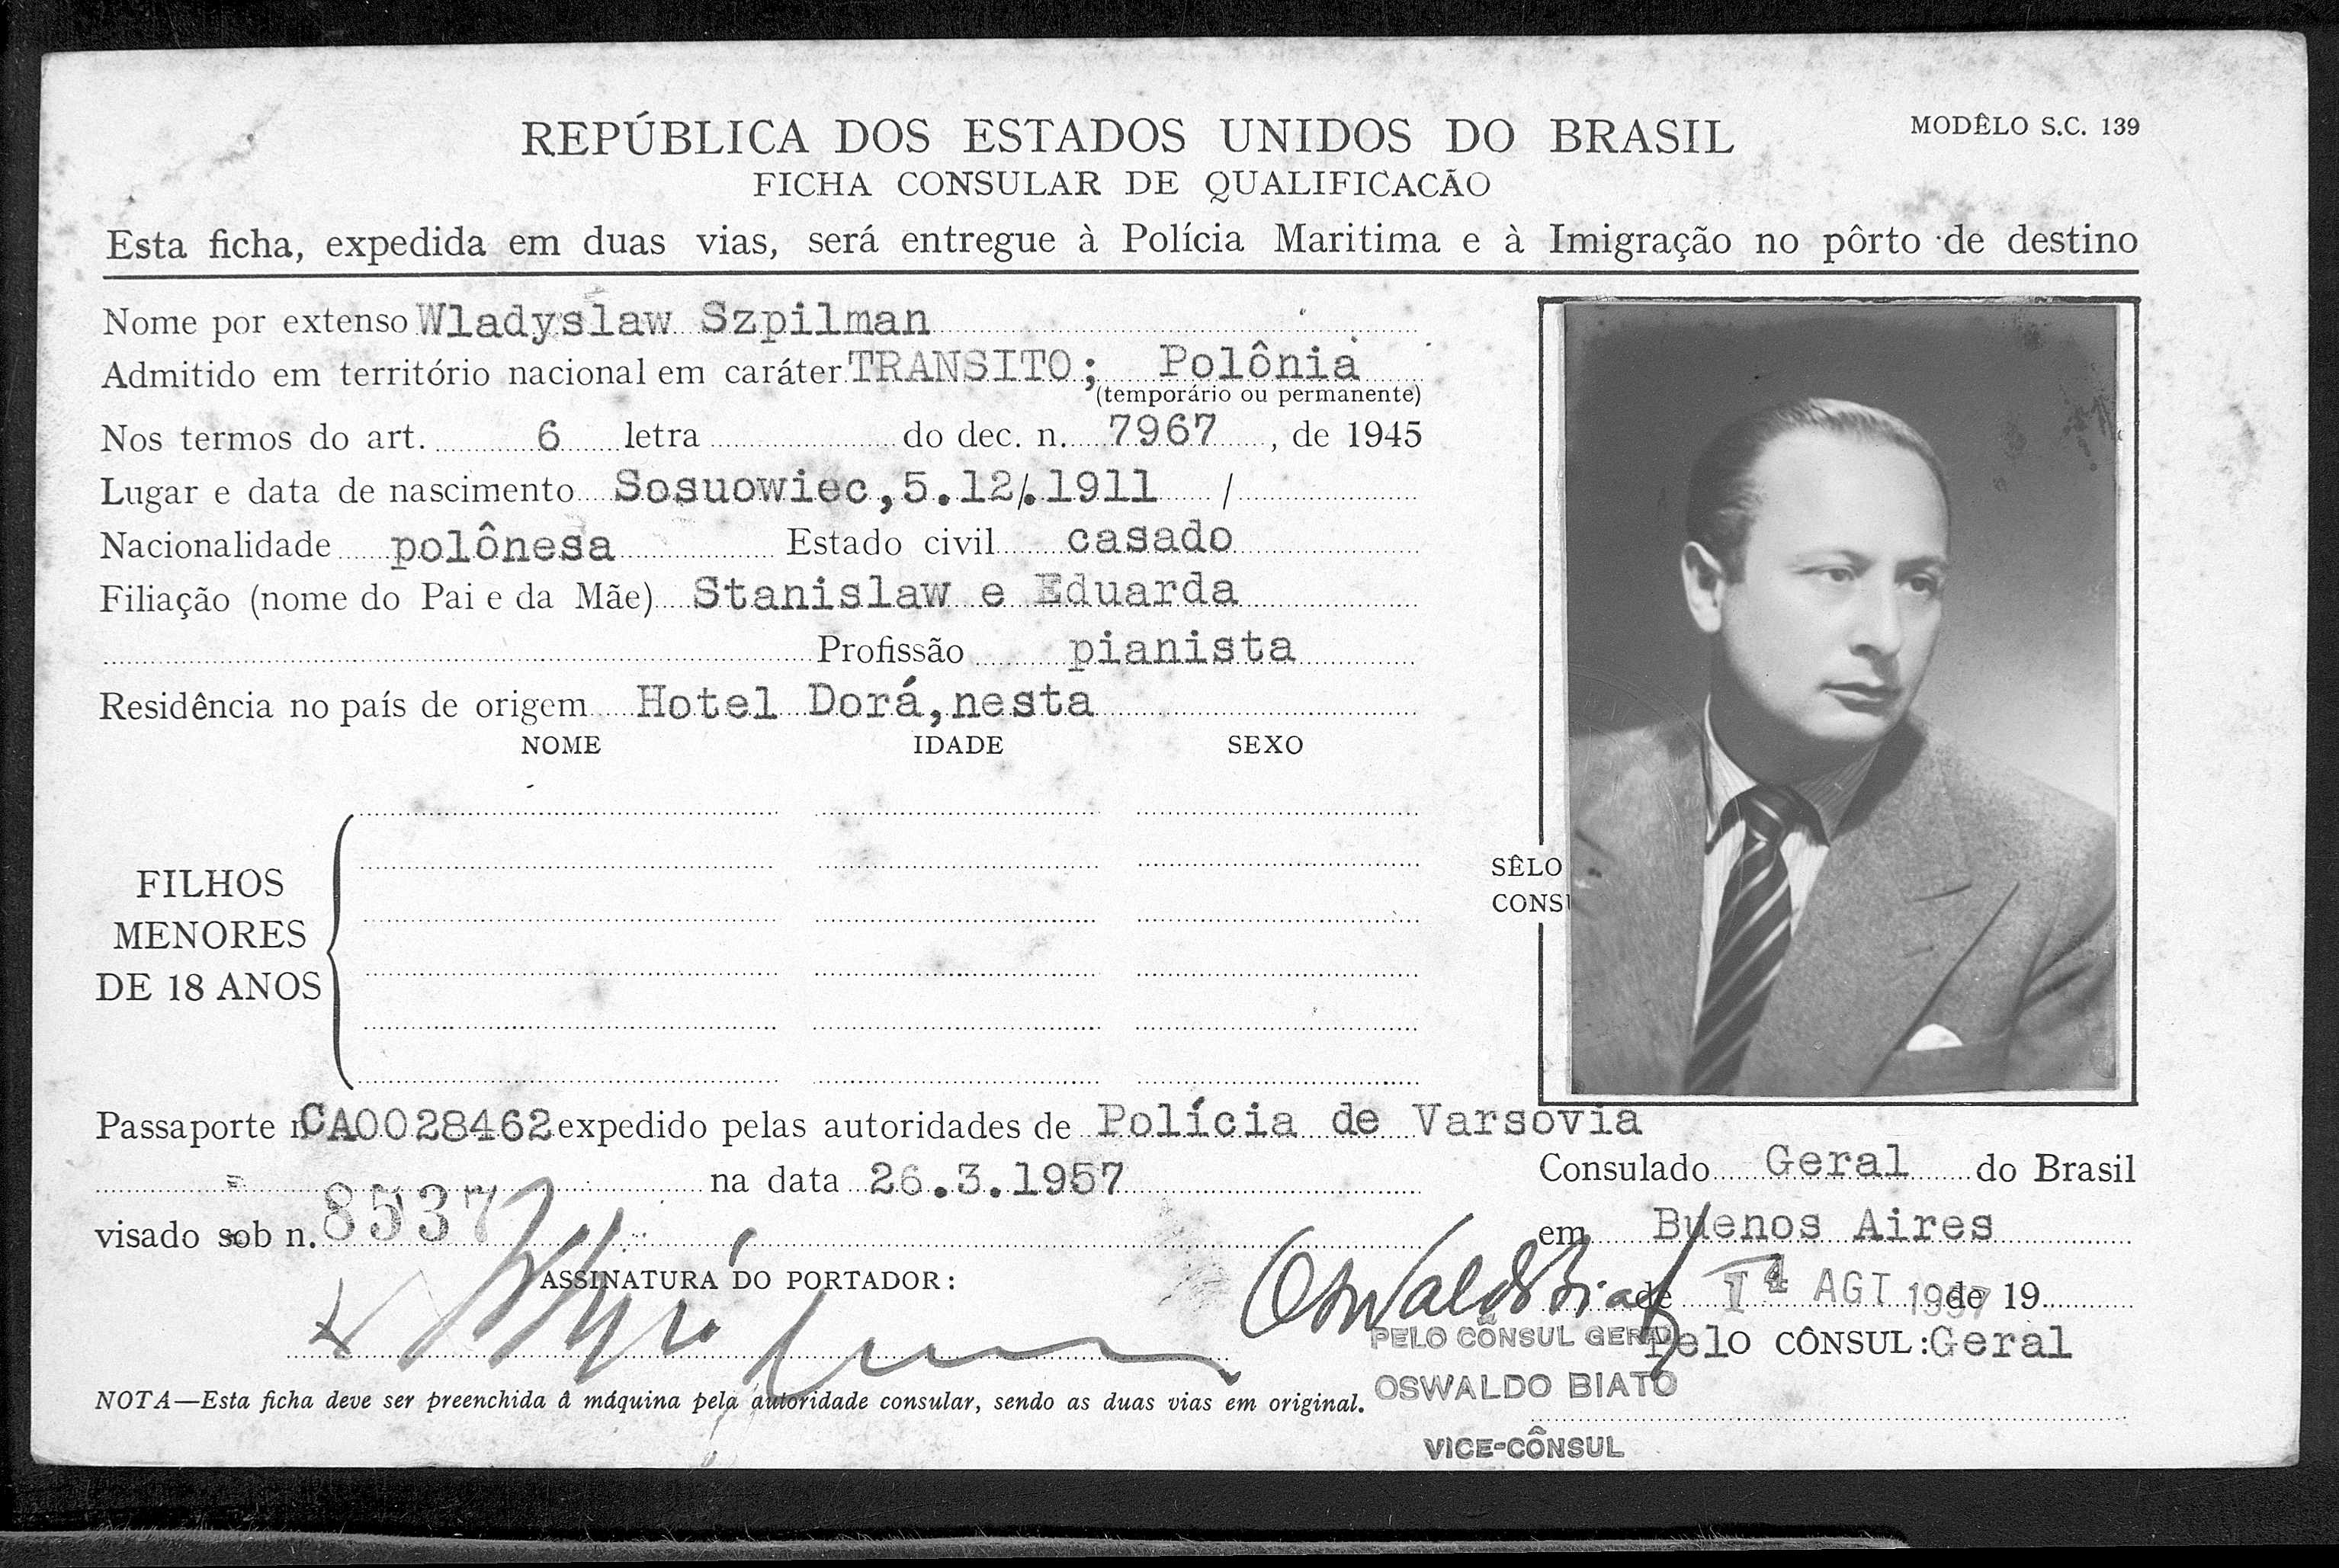
\includegraphics[width=\linewidth]{07/thePianist}
        \centering
        \caption{Registre d'emigració de \emph{Wladyslaw Szpilman}\label{fig:thePianist}}
    \end{figure}

    \section{La gran recessió o altres esdeveniments històrics}

    \paragraph{}
    L'exemple específic que es proposa per aquesta funcionalitat, s'aprofita del fet que es disposa d'un major nombre de registres pels Estats Units que no per la resta de països. Malgrat això, aquesta pot intentar ser reproduïble mitjançant qualsevol altre esdeveniment històric.

    L'objectiu de l'exemple proposat és estudiar els impactes de la gran recessió en la població dels Estats Units a través de les dades de FamilySearch i respondre a la pregunta de si la realitat observada és similar als fets reals.

    Es suggereix a l'estudiant que estudií el nombre de morts i emigracions al voltant d'aquest període com a punt de partida.

    També volem aprofitar aquesta proposta per suggerir als estudiants que qualsevol fet històric, amb un cert impacte, pot intentar ser estudiat a través d'aquesta API. Per aquest motiu, es convida als estudiants a plantejar els seus propis casos d'estudi.

    \section{Comparacions amb els amics o seguidors de Facebook i Twitter}

    \paragraph{}
    L'objectiu d'aquesta funcionalitat és proporcionar a l'usuari, mitjançant les API de FamilySearch, Facebook o Twitter, un conjunt d'eines per tal de comparar les seves dades amb les dels seus amics.

    El nombre de comparacions o eines de cerca a FamilySearch que podrien ser utilitzades és il·limitada, però per donar alguna idea als estudiants del que tenim al cap, en citem algunes a continuació:

    \begin{itemize}
        \item Quin dels nostres amics o seguidors té el nom o cognom més popular en el país on viuen o arreu del món?
        \item Quin dels nostres amics és més probable que tingui ascendència als estats units (per instàncies del cognom en el país)?
        \item Quina diversitat cultural representen les teves amistats?
        \item Mostrar l'esperança de vida mitjana de les persones enregistrades a FamilySearch amb el mateix nom que algun dels nostres amics i comparacions amb aquestes dades.
    \end{itemize}

    Les possibilitats són realment il·limitades i a més a més, l'aplicació podria permetre accions com, seleccionar només els amics que ens interessin per certes consultes, realitzar una cerca sobre tots els nostres amics per localitzar de forma fàcil als que ens interessin, etcètera.

    \section{Comparació de dades genealògiques reals amb FamilySearch}

    \paragraph{}
    Aquesta proposta de projecte pretén validar, en certa forma, com de bé representen les dades de FamilySearch la realitat d'un país o països a través de diferents èpoques, o per una època determinada.

    Aquesta proposta podria ser dividida en molts projectes diferents, un per cada país, concepte o època que l'estudiant vulgui explorar. Per ajudar a comprendre als estudiants al que ens estem referint, a continuació citem una sèrie d'exemples:

    \begin{itemize}
        \item Comparació de mortalitat per infants: Global, per continents, països, èpoques, etcètera.
        \item Mitja de fills per família: Global, per continents, països, èpoques, etcètera.
        \item Edat mitjana de totes les persones enregistrades, en un moment i localització determinades? Evolució d'aquest indicador al llarg del temps.
        \item Proporció d'homes i dones: Global, per continents, països, èpoques, etcètera.
        \item Esperança de vida per les dones i homes: Global, per continents, països, èpoques, etcètera.
    \end{itemize}

    Aquesta proposta no pretén que l'estudiant abordi tots els conceptes diferents que es pugui imaginar, però si en aquells que cregui que poden tenir un valor més elevat de cara a comparar regions i èpoques.

    Segons els factors a estudiar, la complexitat de com hauran de ser processades les dades canvia, i per tant, caldrà tenir-ho en compte a l'hora de definir l'abast del projecte.

    Es recomana també als estudiants que cerquin estudis estadístics sobre la població del món, per poder inspirar-se de cara al plantejament de propostes de projecte. A nosaltres ens va ajudar la presentació a les conferències Ted de Kim Preshoff\footnote{https://www.youtube.com/watch?v=RLmKfXwWQtE}.

    \section{Estudi de profunditat dels arbres familiars}

    \paragraph{}
    Aquesta funcionalitat es basa en l'estudi de les genealogies disponibles a través de FamilySearch.

    Es planteja a l'usuari un estudi de la profunditat d'aquestes, quantes generacions diferents estan emmagatzemades de mitjana, com de completes solen estar les dues bandes de l'arbre familiar, etcètera.

    Un segon conjunt de dades que l'estudi pot intentar respondre és quins són els períodes de temps en els que era més probable mantenir un arbre genealògic. S'està perdent la tradició? Ha anat en augment durant els últims anys? Quina mena d'informació és més probable que es trobi disponible?

    Aquests són alguns dels exemples que plantegem als futurs estudiants.

    \section{Algoritme de marcatge de duplicats}

    \paragraph{}
    FamilySearch té una funció que permet, donada una persona, aconseguir les persones de l'arbre que tenen una alta probabilitat de ser un duplicat.

    L'objectiu d'aquesta aplicació seria realitzar un algoritme, que donada una persona, estudies les persones marcades com a candidates a ser un duplicat  i avalués si aquestes marques tenen pinta de ser correctes o no.

    L'estudiant podria cercar i comparar segons la diferent informació disponible de cada persona i emetre una conclusió final de diferents nivells, com per exemple:

    \begin{itemize}
        \item Insuficient informació per concloure.
        \item Duplicat descartat per inconsistència en els naixements.
        \item Duplicat real amb coincidències de dates de naixement.
        \item Etcètera.
    \end{itemize}

    Un altre aspecte que el projecte podria intentar atacar és comparar la fiabilitat d'aquest algoritme amb la identificació de duplicats per part de FamilySearch.

    Aquest projecte pot resultar bastant complex, i a priori, es desconeix la precisió o condicions sota les quals FamilySearch marca a una persona com a duplicada. Per tant, es recomana realitzar un bon estudi previ d'aquests conceptes abans d'embarcar-se en el projecte.


    \chapter{Estudi tècnic de l'aplicació web}

    \section{Decisió del tipus d'aplicació a implementar}

    \paragraph{}
    Per poder començar a estudiar el conjunt de tecnologies que el projecte requeriria, primer necessitàvem saber quina mena d'aplicació seria implementada.

    Des del principi teníem bastant clar, que de disposar de l’oportunitat, intentaríem implementar una pàgina web. Després de realitzar l’estudi inicial de l’API i de les diferents opcions de desenvolupament possibles, crear una pàgina web semblava l’opció més flexible i factible i per tant, vam decidir tirar per aquest camí.

    La pàgina web representava l’opció més flexible i factible, ja que els protocols per integrar-se amb APIs es troben bastant desenvolupats i a més a més, oferia l’oportunitat d’utilitzar els SDK oficials, així com diverses eines de desenvolupament que facilitarien les tasques de creació i interacció amb usuaris.

    Per tots aquests motius, a part de la motivació personal d’assolir les habilitats necessàries per desenvolupar una aplicació web, escollir aquesta opció tenia tot el sentit del món.

    Així doncs, un cop decidit que s'implementaria una pàgina web, calia fer un reconeixement de les diferents tecnologies disponibles en el mercat i escollir-ne les més adequades, que poguessin treballar de forma conjunta.

    Les tecnologies estudiades poden ser dividides en tres grans blocs: Les tecnologies per la creació d’aplicacions web, tecnologies de desenvolupament i les tecnologies de desplegament.

    Les tecnologies per la creació d’aplicacions web, representen aquell conjunt de llenguatges, arquitectures i frameworks, que serien utilitzats de cara a la construcció de la pàgina web. Amb altres paraules, el conjunt d’eines i llenguatges que s’utilitzaria per implementar el servidor, les comunicacions entre el servidor i l’API de FamilySearch i el frontal o visual de l’aplicació.

    Les tecnologies de desenvolupament, representen el conjunt de tecnologies i eines específiques que han estat utilitzades per assistir i facilitar la creació de l’aplicació web.

    Finalment, les tecnologies de desplegament, fan referència a l'allotjament web escollit i les tecnologies necessàries per poder completar el desplegament de l’aplicació al núvol.

    \section{Tecnologies i patrons utilitzats per l'aplicació web}

    \paragraph{}
    En aquest apartat de la memòria es descriuran el conjunt de patrons de disseny web i tecnologies, que han estat utilitzades per tal que l'aplicació web funcioni i compleixi amb tots els requisits que ens havíem marcat per ella.

    \subsection{El model: Model Vista Controlador}

    \paragraph{}
    A l'hora de crear l’aplicació web, volíem crear-la mitjançant una estructura comprensible i eficient, on cada tecnologia realitzes el seu rol principal i deixés aquelles tasques per les quals no havia estat concebuda, a altres tecnologies.

    En el món del desenvolupament web, sembla que predomina molt una arquitectura de tres capes, que emula bastant bé el model vista controlador. Però, en què consisteix exactament aquest model? El model vista controlador, també conegut com a MVC, és un patró d'arquitectura pensat per la implementació d'aplicacions que disposen d’una interfície d'usuari.

    Com bé indica el nom, el model és compost principalment per tres elements. El Model, la Vista i el Controlador. A continuació, descrivim amb més profunditat el rol de cada un d’aquests components.

    El Model és el principal encarregat de gestionar i manipular les dades amb les quals treballa el sistema. El Model, també s’encarrega de crear la lògica i regles, sobre les que l'aplicació funciona. D’aquesta forma, aquest component serà l’encarregat de gestionar les connexions amb les bases de dades, en cas que es requereixi la utilització d’aquestes, i crearà els blocs de dades a retornar de forma que puguin ser compresos pel Controlador.

    La Vista o Vistes, representen les representacions visuals de la informació. En altres paraules, la interfície que l’usuari veurà i amb la que podrà interactuar. Mitjançant les diferents interaccions possibles amb aquesta, l'usuari és capaç d’indicar a l’aplicació quines són les accions que vol que realitzi.

    Finalment, el Controlador s'encerrega de recollir els diferents inputs enviats per l'usuari, validar-ne l'estat i comunicar-se amb la capa del Model per obtenir les dades o recursos (entesos com a fitxers servits per la capa Model), demanats per l’usuari. En cas de necessitat, el Controlador també és l’encarregat de modificar la vista o l’estat d’una vista, per reflectir en tot moment l’estat de l’aplicació a la interfície d’usuari.

    La gràcia d'aquest model és que l'usuari només disposa d'accés i permisos d'interacció amb la capa de les vistes. Aquestes, comuniquen les accions realitzades per l'usuari al controlador, que a la vegada, s'encarrega de gestionar les comunicacions amb el model i quan aquest retorna dades, transmetre-les a la vista.

    D'aquesta forma, l'ús de la capa model és completament transparent per l'usuari. La figura~\ref{fig:MVC}, mostra un exemple de com podria funcionar el model MVC en un cas ideal. En la nostra aplicació web, intentarem seguir aquest model en la mesura que sigui possible.

    \begin{figure}[h]
        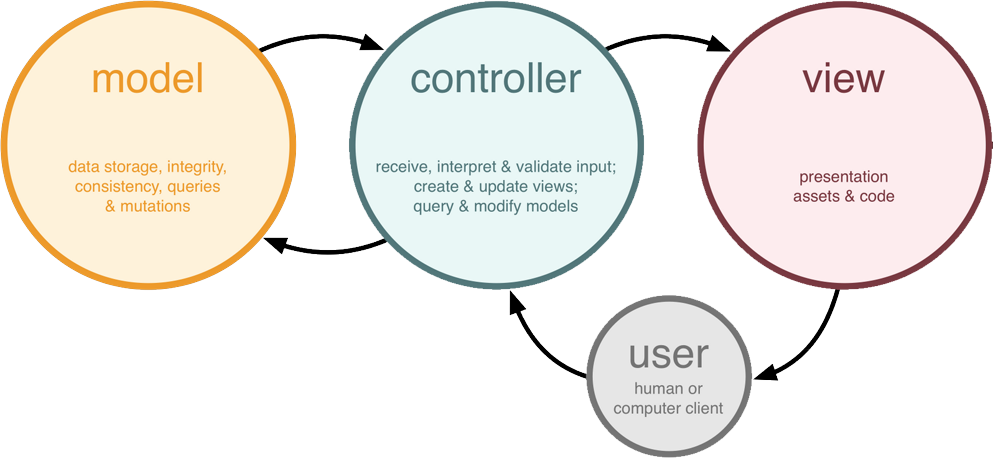
\includegraphics[width=\linewidth]{08/01_MVC}
        \centering
        \caption{Exemple de funcionament del model MVC.}\label{fig:MVC}
    \end{figure}

    Un últim aspecte important, de cara a la terminologia d'aquesta secció de la memòria, és entendre com relacionem cada una de les capes del patrò MVC, amb els elements que conformen una aplicació web.

    Les pàgines web, s'acostumen a poder dividir en dos grans conceptes o elements principals: el front-end i el back-end.

    El front-end, fa referència a la capa de presentació o amb altres paraules, el navegador de l'usuari i per tant, aquest element serà associat a la capa Vista del model MVC.

    Per altra banda, el back-end és el component que acostuma a realitzar l'accés a les dades i tracta la informació que ha de ser servida al front-end. Per tant, en el nostre cas el back-end jugarà el paper de la capa Model en la nostra aplicació web.

    Finalment, el paper del Controlador, sol ser representat en una aplicació web com la part del codi del client (navegador), que l'usuari no veu, ni interactua directament amb ella. En alguns sectors, aquesta part d'una pàgina web es coneix pel nom del `back-end del front-end'.

    La figura~\ref{fig:webElementsEmpty}, mostra els tres elements descrits de les aplicacions web i el paper que jugaran, dins del model MVC, cada un d'ells. Durant els següents apartats d'aquesta secció de la memòria, anirem emplenant cada una de les caixes, amb les diferents tecnologies que seran utilitzades.

    \begin{figure}[h]
        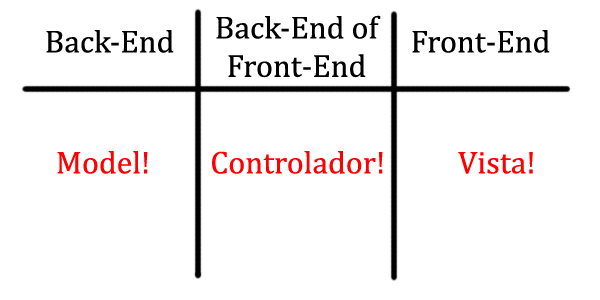
\includegraphics[scale=0.4]{08/02_webTechIni}
        \centering
        \caption{Elements de l'aplicació web i el patro MVC}\label{fig:webElementsEmpty}
    \end{figure}



    \chapter{Javascript SDK Oficial de FamilySearch}

    \section{Introducció}

    \paragraph{}
    Aquest projecte neix de les conversacions amb Enric Mayol mentre explorava diferents opcions sobre quin projecte final de carrera realitzar. L’Enric em va introduir l'organització de FamilySearch i l'existència de la seva \gls{API}, encarregada de gestionar l’accés a les dades d’índole genealògic.

    \gls{FamilySearch} és una organització sense ànim de lucre destinada a connectar famílies a través de generacions. La seva visió com a col·lectiu és el d'ajudar a les persones a crear un vincle amb els seus avantpassats, com a eina per poder comprendre millor qui són, crear un sentiment de família i teixir el pont entre passat i futur.

    Com s'ha esmentat, les dades emmagatzemades per l'organització i accessibles a través de l'\gls{API} són principalment de caràcter genealògic. En concret, es disposa d'una col·lecció de persones de les quals se'n coneix informació personal, esdeveniments rellevants en el transcurs de la seva vida, com podrien ser per exemple dades sobre el seu naixement i les seves relacions amb altres persones, en altres paraules, el seu arbre genealògic.

    El projecte gira entorn aquesta \gls{API} i ha estat dividit en tres grans blocs o seccions.

    Per començar, realitzar un estudi profund de l'\gls{API}.\ Això significa comprendre quines són les petites peces d’informació realment disponibles i com estan relacionades entre elles. D'aquesta forma, també s'ajudarà als futurs estudiants interessats a utilitzar aquesta API, a comprendre-la i poder començar a utilitzar-la, amb molta més facilitat.

    En segon lloc, i com un dels tres blocs principals, utilitzant el coneixement adquirit durant l’estudi de l'\gls{API}, així com les oportunitats i limitacions imposades per la plataforma, conegudes durant la implementació dels exemples, plantejar un conjunt de propostes de projecte que puguin servir a futurs estudiants com a suport i inspiració.

    Finalment, l’últim bloc del projecte consisteix en implementar una aplicació que interactuí amb l'\gls{API} de FamilySearch a través de diferents exemples. L'objectiu dels exemples és el de facilitar l'observació i comprensió del potencial de l'\gls{API}, exposar-ne la informació emmagatzemada i oferir idees sobre com encarar-ne l'explotació.

    \section{Emmascarant les crides REST a l'API de FamilySearch}

    \paragraph{}
    Qualsevol crida que es pretengui realitzar contra l’API de FamilySearch, es realitzarà en el SDK mitjançant una funció Javascript asíncrona que l'emmascara. Això ens permet no haver de preocupar-nos per les URI dels recursos als quals volem accedir o haver d'afegir les capçaleres correctes a cada petició, ja que és el mateix SDK el que s'encarrega de fer-ho i mantenir el conjunt d'URIs als diferents recursos i operacions actualitzat.

    Per exemple, si volem accedir a la persona amb identificador: `KW7S-VQJ', ho podríem fer mitjançant la següent funció.

\begin{lstlisting}[style=rawOwn,caption={Exempla crida emmascarada a l'API de FamilySearch}]
client.getPerson('KW7S-VQJ', {persons:true}).then(function(response) {
    ...
});
\end{lstlisting}

    La variable \emph{client} representa una instància del SDK, l’operació, \emph{getPerson}, l’operació del SDK que volem invocar, l’identificador \emph{KW7S-VQJ} i el JSON \emph{\{persons:true\}}, són els paràmetres a passar a la funció i la variable \emph{response}, és l’objecte que emmagatzemarà la resposta de l’API.

    \section{Implementació basada en Promeses}

    \paragraph{}
    Les promeses són els objectes retornats pels blocs de codi Javascript asíncrons, com per exemple, en la funció de l’apartat anterior, la promesa retornada seria la variable \emph{response}. Una promesa es troba sempre en un dels següents tres estats:

    \begin{itemize}
        \item Pendent: Estat inicial de la promesa.
        \item Satisfeta: L'estat de la promesa representa una operació finalitzada amb èxit.
        \item Rebutjada: L'estat de la promesa representa una operació fallida.
    \end{itemize}

    Tan bon punt una promesa rep l'estat de satisfeta o rebutjada, ja no pot tornar a canviar d'estat.

    La gràcia de les promeses és que tan bon punt són resoltes, permeten executar una part del codi definida amb anterioritat (el que seria el cos de la funció de l'apartat anterior) i mentre aquestes no són satisfetes o rebutjades, la resta del codi pot seguir executant-se. Amb altres paraules, el codi no roman bloquejat mentre espera la resposta de la funció contra l’API.

    \section{Implementació pensada per la programació orientada a objectes}

    \paragraph{}
    Les funcions de crida del SDK, retornen promeses, que no deixen de ser objectes Javascript. Aquests objectes, disposen de funcions de conveniència que permeten accedir als resultats de la resposta sense haver de navegar per objectes de format XML o JSON.

    Per exemple, en la crida de fa dos apartats, podríem obtenir el nom de la Persona cercada, a través de l’objecte response, mitjançant la navegació al recurs de la persona i seguidament, demanant-ne el nom. El següent bloc de codi mostra aquest exemple.

\begin{lstlisting}[style=rawOwn,caption={Example navagació per l'objecte \emph{response}}]
client.getPerson('KW7S-VQJ', {persons:true}).then(function(response) {
    console.log(response.getPrimaryPerson().getDisplayName());
});
\end{lstlisting}

    \section{Model de dades quasi idèntic a FamilySearch}

    \paragraph{}
    Una altra característica destacable del SDK és que implementa un model de dades equivalent al de l’API de FamilySearch, però en aquest cas, pensat per ser navegat mitjançant els estàndards dels llenguatges de programació orientada a objectes, en comptes dels enllaços hypermedia.

    A la figura~\ref{fig:sdkDataModel} podem observar el model de dades proposat pel SDK i com cada un dels objectes es troba relacionat amb els altres.

    \begin{figure}[h]
        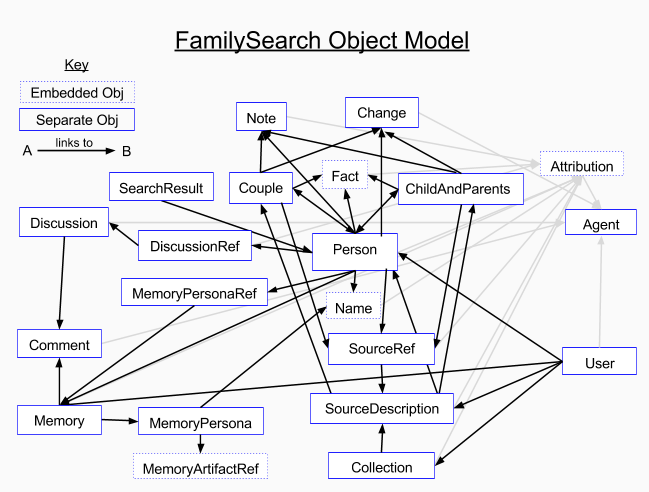
\includegraphics[width=\linewidth]{09/01_objectModel}
        \centering
        \caption{Model de dades del Javascript SDK de FamilySearch}\label{fig:sdkDataModel}
    \end{figure}

    \section{Captura d'errors}

    \paragraph{}
    Els errors de connexió amb l’API són fàcilment tractables gràcies a la naturalesa de les crides asíncrones implementades pel SDK. Només cal afegir la clàusula `.catch' al codi de la petició, tal com es mostra en el següent bloc de codi. La variable \emph{error} és un altre objecte Javascript que conté informació sobre l’error.

\begin{lstlisting}[style=rawOwn,caption={Tractament d'errors amb l'objecte \emph{error}}]
client.getPerson('KW7S-VQJ', {persons:true}).then(function(response) {
    // Tractar les dades retornades per l'API
})
.catch(function(error) {
    // Codi per gestionar l'error
});

\end{lstlisting}

    \section{Intentar de nou peticions GET fallides}

    \paragraph{}
    Els errors de connexió amb l’API són fàcilment tractables gràcies a la naturalesa de les crides asíncrones implementades pel SDK. Només cal afegir la clàusula `.catch' al codi de la petició, tal com es mostra en el següent bloc de codi. La variable error és un altre objecte Javascript que conté informació sobre l’error.

    \section{Gestió automàtica del Throttling}

    \paragraph{}
    Com s'exposava en la quarta secció de la memòria, quan es parlava d'algunes de les funcionalitats extres que l’API de FamilySearch oferia, va ser presentada la funcionalitat de \emph{Throttling}, que evitava que un usuari realitzes `masses' peticions, durant un cert període de temps.

    En cas que l'usuari del SDK sigui bloquejat durant un període de temps per aquesta causa, el mateix SDK, s'encarregarà de gestionar la duració del bloqueig, evitant rellançar la crida fins que aquesta pugui tornar a ser llençada.

    \section{Autentificació mitjançant un pop-up}

    \paragraph{}
    Mentre es realitzi des d'un navegador, l'autentificació d’una aplicació amb FamilySearch, pot ser gestionada mitjançant un pop-up a la pàgina oficial de l’organització.

    D'aquesta forma, no ens hem de preocupar de crear una pàgina de redirecció específica pel protocol OAuth. L'únic requisit, és registrar un URL vàlid, en el mateix domini i port que l’aplicació web, que serà cridada un cop es finalitzi el procés d'identificació a la banda de FamilySearch.

    \section{Autentificació automàtica}

    \paragraph{}
    Existeix l’opció d'activar el protocol d'identificació de forma automàtica, en cas que un usuari intenti realitzar una operació contra l’API sense identificar-se primer, aquesta acció serà demanada abans d’executar la crida. Pot esdevenir útil, ja que les connexions expiren al cap d'un temps d'inactivitat.

    \section{Emmagatzematge del Token en una cookie}

    \paragraph{}
    Existeix l'opció d'emmagatzemar el token d'identificació (retornat per l’operació d'identificació amb FamilySearch) en una cookie.

    Resulta útil de cara a utilitzar el SDK des de la capa del controlador, ja que d’aquesta forma no resulta necessari crear una instància del client a cada pàgina diferent de l’aplicació web o implementar una aplicació web basada en una sola pàgina.

    Malauradament, viola una de les condicions per la certificació de les aplicacions, així que no s'acaba d'entendre perquè apareix en un SDK oficial, mes enllà d'ajuda durant el desenvolupament.

    Per tal d'intentar superar aquesta restricció, en el nostre projecte, hem emmagatzemat el valor del Token en l’espai local del navegador.

    \section{Disparador automàtic de la funció d'expiració}

    \paragraph{}
    Per tal de mantenir la coherència entre l'aplicació web i l'estat de la identificació, recordem que aquesta pot expirar per inactivitat, existeix la possibilitat d'implementar una funció que s'executi quan el token expira.

    D'aquesta forma, podem garantir que en tot moment existeix una concordança d'estat entre el client i el servidor i que per tant, no correm el risc que l'usuari pugui realitzar operacions no permeses en expirar el token d’identificació.

    \section{Utilitzable des de diferents plataformes o capes}

    \paragraph{}
    El SDK és utilitzable tant des del client com el servidor. En altres paraules, pot córrer tant mitjançant la tecnologia Javascript en la capa del controlador, com mitjançant Node.js a la capa del back-end. 

    \section{Suport en el desenvolupament}

    \paragraph{}
    Una de les característiques principals del SDK és que es troba relativament ben documentat. Inclòs m'atreviria a dir, que de cara a obtenir una idea general de com funciona l’API de FamilySearch i quina informació conté, realitza una millor feina que la documentació oficial de l’API. Encara que sigui de forma involuntària, és un punt a destacar.

    Al mateix temps, existeixen diferents grups d'ajuda per aquells desenvolupadors que desitgin utilitzar l'API de FamilySearch i que són visitats de forma regular pels desenvolupadors dels SDK oficials i l’API de FamilySearch.

    Des d'aquesta memòria, es recomana passar pel grup de Google `FamilySearch Developer Network', ja que resulta l'emplaçament ideal per qualsevol dubte que puguem tenir i un centre d'informació ideal sobre el funcionament de l’API i l'estat en què es troba a cada moment.

    \section{Conclusió sobre el SDK}

    \paragraph{}
    Com s'ha pogut observar en les seccions anteriors, són molts els beneficis resultats d'utilitzar un SDK oficial, en comptes de realitzar una implementació directa contra l’API. Per altra banda, el preu a pagar és pràcticament nul, més enllà d'haver d'estudiar el funcionament del SDK, però resulta un esforç rendible.


    \chapter{Introducció a l'aplicació web}

    \paragraph{}
    En aquesta secció de la memòria s’introduiran tots aquells aspectes generals referents a l’aplicació web. En concret, es tractaran els següents punts:

    \begin{itemize}
        \item Accés i codi de l’aplicació web.
        \item Requisits funcionals i no funcionals de l’aplicació web.
        \item Estructura de l’aplicació web.
        \item Estructura de l’aplicació web.
        \item Funcionament general de l’aplicació web.
        \item Detalls específics de la implementació.
        \item Certificació de l’aplicació.
        \item Google Analytics.
        \item Optimització d’imatges.
        \item Hosting de l’aplicació web.
    \end{itemize}

    \section{Accés a l'aplicació web i codi de l'aplicació}

    \paragraph{}
    L’aplicació web es troba desplegada al núvol sota l'URL:

    \begin{displayquote}
        https://pfc-family-search.herokuapp.com/
    \end{displayquote}

    Per accedir a la zona específica d’exemples, la que s’encarrega de mostrar els diferents exemples d’interacció amb l’API, fa falta utilitzar el següent usuari i contrasenya:

    \begin{itemize}
        \item \textbf{Usuari:} tum000145207
        \item \textbf{Contrasenya:} 1234pass
    \end{itemize}

    Per altra banda, el codi de les aplicacions web sol ser extens en nombre de línies i mostrar-lo en aquesta memòria resulta impossible. El codi realitzat ocupa un total de [nombre de línies] repartides un [x\%] en HTML, un [y\%] en Javascript i jQuery i un [z\%] en css.

    Tot el codi de l’aplicació pot ser trobat en el repositori GitHub accessible a través del següent URL:

    \begin{displayquote}
        https://github.com/sinh15/pfc-family-search
    \end{displayquote}

    L’estructura del codi serà presentada més endavant, en aquesta mateixa secció de la memòria, però principalment, el servidor està compost pel fitxer \emph{app.js}, els fitxers HTML es troben a la carpeta \emph{views} i els fitxers Javascript i jQuery, a la carpeta \emph{assets}.

    \section{Requisits de l'aplicació web}

    \paragraph{}
    Aquesta llista pretén oferir un tast dels requisits o manaments que s'han tingut en compte durant el desenvolupament de l'aplicació web.

    \subsection{Requisits funcionals}

    \begin{itemize}
        \item La web ha de permetre identificar-se amb FamilySearch mitjançant el sistema d'autentificació per pop-up.
        \item La web ha de permetre a l'usuari tancar la connexió amb FamilySearch mitjançant una funcionalitat de `Sign Out'.
        \item L'aplicació ha de ser capaç de tancar automàticament la connexió amb FamilySearch si aquesta expira.
        \item La web ha d'incloure una secció que ofereixi un petit resum del rerefons que va originar el projecte.
        \item La web ha de disposar d'una secció en què s'enumerin i exposin les diferents propostes de projecte generades pels futurs estudiants.
        \item L'aplicació ha d'oferir la possibilitat de cercar persones en l'arbre familiar de FamilySearch i observar-ne els detalls d'alguna en concret.
        \item L'aplicació ha de permetre a l'usuari observar l'evolució geogràfica d'un cognom donat un conjunt de països i període de temps.
        \item L'aplicació ha de permetre la visualització del nombre de naixements, casaments i defuncions enregistrades per un país al voltant d'un any concret.
        \item La secció d'exemples ha de ser només accessible si l'usuari es troba identificat a FamilySearch i ha rebut el token d'ús pertinent.
        \item En cas que el token expiri, l'usuari ha de ser redirigit a la pàgina principal en el moment d'expiració o en la seva següent interacció si aquest es troba dins de l'àrea d'exemples.
        \item L'aplicació ha d'emmagatzemar el token proporcionat per FamilySearch que rep l'usuari en un recurs que no sigui accessible ni modificable per tercers.
        \item No es permetrà a l'usuari llençar dues crides contra l’API de FamilySearch simultànies per la mateixa funcionalitat des de la mateixa pestanya del navegador.
        \item L’aplicació ha d'aportar la informació bàsica sobre l’origen del projecte i el seu rerefons. L'aplicació també ha d’enllaçar en algun lloc amb el codi font del projecte.
    \end{itemize}


    \subsection{Requisits no funcionals}

    \begin{itemize}
        \item L'aplicació web ha de funcionar i ser visualitzada de forma correcta en els principals navegadors web moderns.
        \item Els formularis de l'aplicació web que puguin generar errors han de proporcionar informació bàsica a l'usuari en el moment que el camp és abandonat o informació més detallada si envia el formulari amb errors.
        \item Els formularis de l’aplicació han de donar un feedback positiu en cas que els camps siguin omplerts de forma correcta.
        \item La web ha de ser relativament fàcil d'utilitzar, oferint les eines necessàries als usuaris i facilitant la navegació per les diferents seccions.
        \item Mentre l'aplicació web espera resposta de l’API de FamilySearch, s'ha de mostrar a l'usuari que l'aplicació es troba esperant resultats i el progrés realitzat fins al moment.
        \item L'aplicació ha de donar un feedback clar a l'usuari quan la interacció amb l’API de FamilySearch finalitza.
        \item L'aplicació ha de ser navegable de forma acceptable mitjançant dispositius mòbil. Les integracions amb l’API de FamilySearch també han de ser utilitzables, però no cal que la informació resultant es trobi completament adaptada a aquests dispositius.
        \item Les imatges de l'aplicació s'han de trobar optimitzades en la mesura que sigui possible per intentar que aquesta carregui el més ràpid possible en un entorn d'hostalatge gratuït.
        \item Les imatges principals de l'aplicació s'han de carregar de formar transparent quan l'aplicació és iniciada i la primera pàgina és carregada, per millorar la visualització de la web quan l'usuari navega entre les diferents seccions.
        \item La llengua utilitzada en el web serà l'anglès per tal d'ajudar i facilitar el procés de certificació.
        \item El projecte s'ha de trobar sota una certificació Creative Commons d'atribució no comercial.
        \item La informació sobre el codi font del projecte, la llicència i la facultat d'informàtica ha de trobar-se disponible en el peu de pàgina de les pàgines de la web.
        \item Es podrà monitorar la navegació dels usuaris pel web, així com les seves accions principals i errors generats.
        \item Es podrà obtenir la configuració dels sistemes amb els quals s'ha navegat per la web i veure si el comportament d'algun d'ells és més propici a la generació d'errors.
        \item Els fitxers Javascript s'han de trobar el més al final possible dels arxius HTML per facilitar la càrrega del contingut.
        \item Es reutilitzarà codi HTML i Javascript en la mesura que sigui possible per tal d'evitar la duplicació de contingut.
    \end{itemize}

    \section{Estructura de l'aplicació web}

    \subsection{Introducció a l'estructura de l'aplicació}

    \paragraph{}
    L'aplicació web és relativament simple pel que respecta a la navegació i les diferents seccions que la conformen.

    La figura~\ref{fig:webStructure} mostra l'arbre de continguts accessibles. Cal indicar, que aquesta figura no representa les úniques rutes de navegació existents entre les diferents seccions, sinó un breu mapa del contingut total disponible a través del web i d’on penja cada secció.

    \begin{figure}[h]
        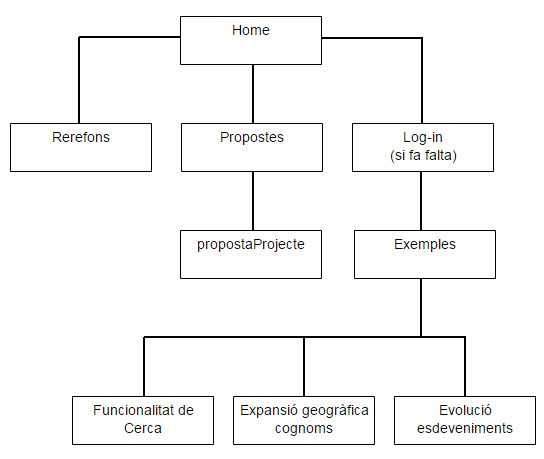
\includegraphics[scale=0.6]{10/01_estructuraWeb}
        \centering
        \caption{Diferents seccions de l'aplicació web}\label{fig:webStructure}
    \end{figure}

    Més endavant, s’explicarà més en detall en què consisteix cada una de les pàgines o seccions de la nostra aplicació web, però primer volem presentar l'estructura general o esquelet, que segueixen gairebé totes les pàgines del nostre web.

    La figura~\ref{fig:pageStructure} mostra l'esquema bàsic sobre el qual les pàgines són construïdes. Aquest pot ser descrit o desglossat en les següents seccions:

    \begin{enumerate}
        \item \textbf{Barra de navegació:} Permet desplaçar-se per les diferents seccions principals.
        \item \textbf{Capçalera de secció:} Conté el títol i subtítol de la pàgina sobre impressionat a una imatge relacionada.
        \item \textbf{Contingut principal:} El contingut principal i únic d'aquesta pàgina.
        \item \textbf{Footer:} Peu de pàgina. Inclou informació sobre el codi font del projecte, la llicència i la facultat d'informàtica de Barcelona.
    \end{enumerate}

    \begin{figure}[h]
        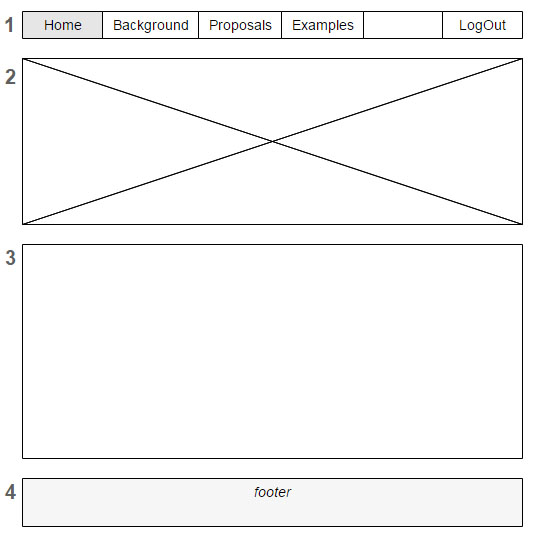
\includegraphics[scale=0.6]{10/02_pagesStructure}
        \centering
        \caption{Esquema bàsic de les pàgines implementades en el domini web}\label{fig:pageStructure}
    \end{figure}

    Convidem des de la memòria, als usuaris de l'aplicació web, a redimensionar la finestra web per tal d'observar com els continguts de cada pàgina s’adapten al dispositiu que els mostra.

    A continuació descriurem el contingut de cada secció o apartat que conforma la nostra aplicació web.

    \subsection{Home o pàgina principal}

    \paragraph{}
    La home és la primera pàgina que veu l'usuari quan entra a l'aplicació web. Aquesta no té cap altre propòsit que el de donar la benvinguda i enllaçar als diferents continguts.

    El bloc de contingut principal d’aquesta pàgina inclou enllaços i breus descripcions, a les tres seccions principals del projecte. A saber: rerefons, propostes de projecte i exemples d'implementació.

    La principal diferència entre la versió per dispositius mòbils i la d'escriptori és que la primera fa desaparèixer el subtítol, simplifica el títol, transforma la barra de navegació en una usable per dispositius mòbil i transforma la secció de contingut principal apilant-ne el contingut de cada una de les tres columnes que la conformen.

    \subsection{Rerefons}

    \paragraph{}
    La pàgina de rerefons conté la informació bàsica respecte a l'origen, context i motivacions, que ens van portar a realitzar aquest projecte. Consisteix en un breu resum, molt superficial, d’alguns dels apartats exposats en la primera secció de la memòria.

    El bloc de contingut principal d'aquesta pàgina consisteix en dos grans blocs de text. El primer, descriu el rerefons del projecte, mentre que el segon ofereix una petita descripció del context i motivacions.

    La principal diferència entre les versions d'escriptori i mòbil és que la segona presenta un títol més simple, la desaparició del subtítol i una barra de navegació adaptada a dispositius mòbils. L'estructura del contingut roman igual, això si, adaptat a la grandària del dispositiu que el conté. 

    \subsection{Propostes de projecte}

    \paragraph{}
    L'apartat de propostes de projecte recull les diferents propostes que han estat generades per servir com a projectes finals de carrera pels estudiants d'informàtica.

    El bloc de contingut principal per aquesta pàgina consisteix en dos blocs composts per petites caixes que contenen una imatge, un títol i una petita descripció de la proposta que representen. Cada una d'aquestes caixes enllaça també amb una pàgina que conté alguns detalls de la proposta.

    El primer bloc de caixes representa les propostes generades pels futurs estudiants, mentre que el segon bloc està format per les propostes relacionades amb els exemples implementats.

    Les principals diferencies entre les versions d'escriptori i dispositius mòbils, és que la segona presenta un títol simplificat, la desaparició del subtítol, la barra de navegació adaptada i diferent nombre de caixes per fila segons el dispositiu utilitzat. Tres columnes per escriptoris, dues per tauletes gràfiques i una per mòbils.

    \subsection{Detalls específics d'una proposta de projecte}

    \paragraph{}
    Com bé indica el nom de la secció, aquesta pàgina mostra els detalls específics de la proposta seleccionada des de la pàgina propostes.

    Les diferents propostes són totes generades des del mateix document HTML. És en aquest cas el servidor, l'encarregat d'enviar un conjunt d'informació diferent segons la proposta que ha estat seleccionada. Veurem en més detall com aquest procés funciona en futurs apartats d’aquesta secció.

    El bloc del contingut principal per cada una de les propostes, està conformat per una breu descripció del projecte i en alguns casos, certs exemples, preguntes o possibilitats d’extensió, que la proposta pot abordar. Les propostes també disposen d’una petita valoració numèrica, que representa una valoració de la dificultat d’execució de la proposta. Com més gran és el valor, més complexa.

    La versió d'escriptori i mòbil no es diferencien en grans aspectes excepte en l'adaptació del contingut a la pantalla del dispositiu i els típics canvis esmentats en els apartats anteriors sobre el títol, subtítol i barra de navegació.

    \subsection{Identificació amb FamilySearch}

    \paragraph{}
    Aquesta pàgina s'utilitza per assegurar que l'usuari no pot utilitzar els exemples sense identificar-se abans amb l’API de FamilySearch.

    La pàgina apareix quan l'usuari intenta accedir a la pàgina d'exemples o la pàgina d'un exemple en concret, però encara no s’ha identificat amb FamilySearch. La pàgina permet dues accions simples, tornar enredera (o a la home si s'ha accedit a la pàgina mitjançant la introducció directa de l'URL) o identificar-se amb FamilySearch.

    El procés d'identificació s'inicia mitjançant el llançament d'un pop-up, que obre la pàgina de FamilySearch. Aquesta demana la introducció del nom d'usuari i contrasenya. Un cop aquesta informació ha estat verificada, el servidor redirigeix a l'usuari a la pàgina que havia demanat accedir.

    La pàgina d'identificació tampoc pateix cap reestructuració especial del contingut quan es veu amb dispositius més petits. Simplement, s'adapta a la pantalla que la mostra i reorganitza els botons que permeten tornar endarrere o obrir el procés d’identificació.

    \subsection{Exemples implementats}

    \paragraph{}
    La pàgina d'exemples implementats permet a l'usuari descobrir les diferents eines que han estat implementades, per demostrar possibles interaccions amb l’API de FamilySearch i accedir a cada una d'elles.

    El bloc de contingut principal, segueix un estil molt similar a la pàgina propostes de projecte, descrita tres apartats endarrere. Aquesta, mostra per cada un dels exemples implementats un títol, una breu descripció i permet a l'usuari navegar cap a les pàgines que contenen les implementacions concretes.

    Les principals diferencies entre les versions d'escriptori i dispositius mòbils són exactament les mateixes que per la pàgina de propostes de projecte. És a dir, títol adaptat, eliminació del subtítol, adaptació de la barra de navegació i nombre de propostes per fila segons la grandària del dispositiu.

    Realment, aquestes dues pàgines tenen un comportament tècnic idèntic i l'únic que les diferencia és el concepte semàntic que representen i en conseqüència, el contingut.

    \subsection{Funcionalitats de cerca, expansió geogràfica d'un cognom i evolució d'esdeveniments}

    \paragraph{}
    Aquestes pàgines segueixen el mateix patró que la gran majoria de pàgines web de l’aplicació. Recordem que l'esquelet d’aquestes pàgines es mostrava en la figura\ref{fig:pageStructure} d'aquesta mateixa secció de la memòria.

    La gran diferencia, d'aquestes pàgines amb la resta és que la part del contingut principal és relativament més complexa i diferent per cada una d'elles. És per aquest motiu, que el comportament exacte de cada una d'aquestes pàgines serà exposat per separat a la secció onze de la memòria.

    Pel que fa a l'estructura en comú que comparteixen amb la resta de pàgines, les diferències entre la visualització entre dispositius mòbils i escriptori són les ja conegudes: minimització del títol, desaparició del subtítol i adaptació de la barra de navegació.


    \section{Fitxers de l'aplicació web i la seva funcionalitat}

    \paragraph{}
    En aquest apartat de la memòria volem presentar l'arbre d'arxius generats per tal de programar la pàgina web i exposar la funció que desenvolupa cada un d'ells en el marc de l'aplicació.

    Recordem que tot el codi programat per tal de fer funcionar l’aplicació web pot ser trobat a l'URL:

    \begin{displayquote}
        https://github.com/sinh15/pfc-family-search
    \end{displayquote}

    El conjunt de fitxers programats, representa un total de [línies codi] línies de codi, de les quals un XX\% són codi HTML, un XX\% codi Javascript i un X\% codi CSS.

    La taula~\ref{tab:codeFiles} mostra la localització relativa de cada arxiu i en descriu breument la seva funcionalitat.

    \begin{center}
             \csvreader[
                separator=comma,
                before table=\sffamily\small,
                longtable={p{4cm-2\tabcolsep}p{10cm-2\tabcolsep}},
                table head={\caption{Fitxers de codi de l'aplicació web}\label{tab:codeFiles}\\\toprule%
                    \headentry{m{4cm-2\tabcolsep}}{Arxiu}
                    & \headentry{m{10cm-2\tabcolsep}}{Funció}\\\midrule},
                late after line=\\\midrule,
                late after last line=\\\bottomrule,
             ]
             {./tables/10/codeFiles.csv}
             {name=\name,desc=\desc}
             {\name&\desc}
     \end{center}

    \section{Funcionament general de l'aplicació web}

    \paragraph{}
    L'objectiu d'aquest apartat és explicar com els diferents components de la web interactuen entre ells per tal de crear l'aplicació web desplegada al núvol.

    Com a suport a les explicacions que s'oferiran, la figura~\ref{img:appWorkflow} mostra un diagrama amb els components principals de l'aplicació, com interactuen entre ells i els principals formats de dades que intercanvien.

    \begin{figure}
        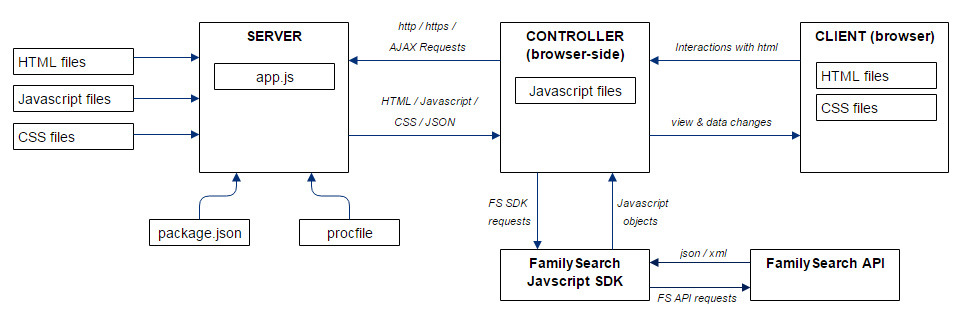
\includegraphics[scale=0.6, angle=90]{10/03_applicationWorkingFlow}
        \centering
        \caption{Comunicació entre els diferents components de l'aplicació web}\label{img:appWorkflow}
    \end{figure}

    En la imatge es poden observar les capes Servidor, Controlador i Client, que conformen l'arquitectura en tres capes explicada en seccions anteriors. També es pot observar el Javascript SDK, del que es detalla com es comunica amb l'API de FamilySearch i a quina capa de l'aplicació es troba connectat.


    \subsection{Creació del servidor}

    \paragraph{}
    L'aplicació comença a funcionar quan aquesta és executada en els servidors al núvol de Heroku, la plataforma d'hostalatge. La configuració del servidor es realitza mitjançant els fitxers \emph{Procfile} i \emph{package.json}, que s'encarreguen d'assegurar que tots els complements Javascript necessaris siguin instal·lats i s'executi el fitxer \emph{app.js} per arrancar i configurar el servidor.

    Quan la configuració del servidor acaba, aquest es troba preparat per començar a rebre peticions dels usuaris.


    \subsection{Accés a una pàgina del domini web}

    \paragraph{}
    Quan un usuari demana carregar la pàgina inicial de la nostra aplicació, una petició HTTP o HTTPS és generada i enviada cap al servidor a través del navegador del client.

    Quan el servidor la rep, l'avalua i en cas d'èxit, retorna al client els fitxers processats necessaris perquè el navegador pugui mostrar la pàgina demanada i carregar totes les funcionalitats o interaccions possibles d'aquesta al controlador.


    \subsection{Interacció amb l'API de FamilySearch}

    \paragraph{}
    El moment en què l'usuari vol interactuar amb l'API de FamilySearch, aquest es veu forçat a interactuar primer amb un element del codi HTML per comunicar l’acció a realitzar. Per exemple, el botó de cerca de la funcionalitat d'evolució temporal d'esdeveniments.

    Quan el controlador detecta que el botó de cerca ha estat pressionat, captura l'esdeveniment i avalua la petició. En cas que no es detecti cap problema ni error en els paràmetres introduïts, el controlador realitza una crida asíncrona al SDK de FamilySearch i n'espera la resposta.

    De forma transparent a l'aplicació web, el SDK es comunica amb l’API de FamilySearch i si no hi ha cap problema en la comunicació i la petició és vàlida, aquesta retorna les dades demanades en format XML o JSON. Posteriorment, el SDK transforma la resposta de l’API en un objecte Javascript amb funcions de conveniència que facilitaran l'accés a les dades de la resposta i el retorna al controlador.

    En el moment que el SDK retorna l'objecte, la promesa pendent de resolució que havia creat el controlador és resolta i l'objecte retornat pel SDK passa a ser accessible. Arribats a aquest punt, el controlador processa i transforma les dades contingudes a l'objecte de la forma desitjada i un cop finalitzades les operacions necessàries, modifica la vista del client introduint els canvis pertinents en aquesta.


    \subsection{Interacció amb elements del HTML}

    \paragraph{}
    Quan els usuaris interactuen amb elements bàsics del HTML, per exemple, quan interactuen amb les caixes que permeten expandir o plegar seccions del formulari en les funcionalitats de cerca o evolució geogràfica de cognoms, la resposta a realitzar per part del controlador és bastant simple.

    En el moment que el controlador detecta que s'ha interactuat amb algun dels elements que escolta, captura l'esdeveniment, avalua com s'ha de procedir segons el context de l'acció, en el cas de l’exemple, plegar o desplegar contingut d'un formulari i realitza de forma immediata els canvis a la vista del navegador.


    \subsection{Conclusió}

    \paragraph{}
    Els casos d'ús que s'han cobert en els apartats anteriors són relativament simples, però són una mostra representativa del conjunt d'accions diferents a les quals l'aplicació pot haver de fer front.

    Esperem que aquesta secció hagi servit per il·lustrar el funcionament general de la web i com els diferents components interactuen entre ells. La resta d’accions possibles en el web, requerint més o menys complexitat per part del controlador, segueixen una de les tres rutes descrites en els apartats anteriors, per tal de ser satisfetes.

    \section{Detalls específics de la implementació}

    \section{Introducció}

    \paragraph{}
    Aquest projecte neix de les conversacions amb Enric Mayol mentre explorava diferents opcions sobre quin projecte final de carrera realitzar. L’Enric em va introduir l'organització de FamilySearch i l'existència de la seva \gls{API}, encarregada de gestionar l’accés a les dades d’índole genealògic.

    \gls{FamilySearch} és una organització sense ànim de lucre destinada a connectar famílies a través de generacions. La seva visió com a col·lectiu és el d'ajudar a les persones a crear un vincle amb els seus avantpassats, com a eina per poder comprendre millor qui són, crear un sentiment de família i teixir el pont entre passat i futur.

    Com s'ha esmentat, les dades emmagatzemades per l'organització i accessibles a través de l'\gls{API} són principalment de caràcter genealògic. En concret, es disposa d'una col·lecció de persones de les quals se'n coneix informació personal, esdeveniments rellevants en el transcurs de la seva vida, com podrien ser per exemple dades sobre el seu naixement i les seves relacions amb altres persones, en altres paraules, el seu arbre genealògic.

    El projecte gira entorn aquesta \gls{API} i ha estat dividit en tres grans blocs o seccions.

    Per començar, realitzar un estudi profund de l'\gls{API}.\ Això significa comprendre quines són les petites peces d’informació realment disponibles i com estan relacionades entre elles. D'aquesta forma, també s'ajudarà als futurs estudiants interessats a utilitzar aquesta API, a comprendre-la i poder començar a utilitzar-la, amb molta més facilitat.

    En segon lloc, i com un dels tres blocs principals, utilitzant el coneixement adquirit durant l’estudi de l'\gls{API}, així com les oportunitats i limitacions imposades per la plataforma, conegudes durant la implementació dels exemples, plantejar un conjunt de propostes de projecte que puguin servir a futurs estudiants com a suport i inspiració.

    Finalment, l’últim bloc del projecte consisteix en implementar una aplicació que interactuí amb l'\gls{API} de FamilySearch a través de diferents exemples. L'objectiu dels exemples és el de facilitar l'observació i comprensió del potencial de l'\gls{API}, exposar-ne la informació emmagatzemada i oferir idees sobre com encarar-ne l'explotació.

    \subsection{Estructura general d'una pàgina HTML:\@Mustache\@I}

    \paragraph{}
    A excepció de la pàgina d'identificació amb FamilySearch, la resta de pàgines de l'aplicació web segueixen la mateixa estructura, tal com s'ha exposat en l'apartat Estructura de l'aplicació web.

    Per evitar la duplicació de codi entre les diferents pàgines, els elements compartits han estat creats en fitxers separats i són carregats a cada pàgina segons si volem mostrar-los o no. Recordem que la tecnologia utilitzada, que fa això possible, és el llenguatge de plantilles Mustache.

    L'esquelet del codi d'una pàgina qualsevol del nostre web segueix la forma mostrada en el bloc de codi que segueix.

    \begin{lstlisting}[style=rawOwn,caption={Exemple d'inclusió de fitxers HTML amb Mustache}]
<!-- header includes -->
{{> header }}
{{> navbar }}
{{> pageTitle }}
<!-- specific page content -->
...
{{> javascripts }}
<!-- specific javascripts for this file -->
...
<!-- footer -->
{{> footer }}
    \end{lstlisting}

    Les etiquetes \emph{\{\{> fileName\}\}}, s'utilitzen per indicar que es vol importar, en aquesta posició, el codi HTML del fitxer \emph{fileName.html}.

    Mitjançant aquesta estructura tenim el control absolut de quins components volem incloure a cada una de les pàgines. Per exemple, l'esquelet de la pàgina d'identificació, es diferencia de la resta en el fet que no s'inclouen els fitxers \emph{navbar}, \emph{pageTitle} ni  \emph{footer}.

    També cal destacar que abans del \emph{footer}, deixem un espai en blanc, per incloure fitxers Javascript que són utilitzats únicament per la pàgina carregada, d'aquesta forma s'evita carregar tots els controladors a totes les pàgines, si aquests no han de ser utilitzats.

    \subsection{El fitxer header.html: Configuració de la pàgina}

    \paragraph{}
    Aquest fitxer s'encarrega de configurar la capçalera de les pàgines del nostre domini i obrir el cos del codi. També es declaren en aquesta secció els arxius CSS a carregar i les fonts a utilitzar.

    Les línies de codi més interessants són les que configuren el `viewport' del dispositiu, perquè aquest s'adapti de forma adequada a qualsevol pantalla i l'etiqueta necessària per indicar al navegador la codificació en què es troben els caràcters (línies 1 i 4 del següent codi).

    \begin{lstlisting}[style=rawOwn,caption={Capçaleres incloses en el fitxer header.html}]
<meta charset=`utf-8'>
<meta http-equiv=`X-UA-Compatible' content=`IE=edge'>
<title>PFC - Family Search API Study</title>
<meta name=`viewport' content=`width=device-width, initial-scale=1'>
<link href=`/node_modules/.../bootstrap.min.css' rel=`stylesheet'>
<link href=`/assets/css/style.css' rel=`stylesheet'>
<link href=`fontNumber1' rel=`stylesheet' type=`text/css'>
<link href=`fontNumber2' rel=`stylesheet' type=`text/css'>
    \end{lstlisting}

    \subsection{El fitxer navbar.html: La barra de navegació adaptativa}

    \paragraph{}
    Com el nom del fitxer indica, aquest s'encarrega de configurar la barra de navegació. Aquesta ha estat creada mitjançant la potencialitat d'un dels components de Bootstrap.

    Consta principalment de dos blocs de codi HTML. El primer, s'utilitza per indicar la capçalera de la barra de navegació, que conté el botó per expandir-la en dispositius mòbils, la icona de l'aplicació que es mostra només en dispositius d'escriptori i el nom de l'aplicació web.

    La capçalera adaptativa de Bootstrap, per la barra de navegació, s'invoca mitjançant la classe \emph{navbar-header}.

    \begin{lstlisting}[style=rawOwn,caption={Capçalera de la barra de navegació}]
<div class=`navbar-header'>
    <button class=`navbar-toggle collapsed'>...</button>
    <a href=`/'><img src=`/images/littleIco.png'/></a>
    <a class=`navbar-brand navbar-link' href=`/'>FamilySearch-PFC</a>
</div>
    \end{lstlisting}

    El segon bloc, s'encarrega de generar els enllaços a les diferents seccions de l'aplicació i configurar el botó dedicat al tancament de la connexió amb FamilySearch, si aquesta està oberta.

    Cada enllaç és estilitzat i configurat mitjançant la classe \emph{navbar-link}. Per decidir si un enllaç ha d'aparèixer per l'esquerra o dreta de la barra de navegació, es mira la inclusió de la classe navbar-righ en el contenidor dels enllaços.

    \begin{lstlisting}[style=rawOwn,caption={Enllaços de la barra de navegació}]
<div class=`collapse navbar-collapse' id=`...'>
	<ul class=`nav navbar-nav'>
		<li><a class=`navbar-link' href=`/background'>Background</a></li>
		<li><a class=`navbar-link' href=`/proposals'>Proposals</a></li>
		<li><a class=`navbar-link' href=`/examples'>Examples</a></li>
	</ul>
	<ul class=`nav navbar-nav navbar-right'>
		<li><a id=`signOut' class=`navbar-link' href>Sign Out</a>
	</ul>
</div>
    \end{lstlisting}

    \subsection{El fitxer pageTitle.html: Mustache II}

    \paragraph{}
    El fitxer \emph{pageTitle.html} resulta un dels fitxers HTML més interessant de l'aplicació. Com s'ha comentat en el primer apartat d'aquesta secció, quasi totes les pàgines de l'aplicació contenen el bloc de codi que hem anomenat `capçalera de secció'.

    Aquesta capçalera consta d'una imatge de fons, amb un títol i subtítol superposats segons el dispositiu des del qual s'accedeix a la pàgina. Els paràmetres que marquen la imatge de fons, els texts, el color del ressaltat i si cal mostrar un botó de navegació o no, són enviats pel servidor i carregats de forma dinàmica segons la pàgina visitada.

    Recordem que les etiquetes \emph{\{\{nomEtiqueta\}\}} són referències a codi Mustache i representen paràmetres dinàmics emplenats pel servidor abans de servir el HTML. En el bloc de codi que es mostrarà més endavant, es podran veure importats els paràmetres: backgroundImage, \emph{highlight}, \emph{title}, \emph{subtitleDesktop}, \emph{subtitleTabet} i \emph{button}.

    Fixem-nos també en el fet que aquests paràmetres poder ser importants a qualsevol lloc del codi HTML. En alguns casos, s'importen com a classe d'un element HTML, indicant-ne l'estil i comportament esperat i altres, simplement, es tracta de contingut estàtic, com per exemple, el títol.

    Destacar també, que pot resultat interessant fixar-se en com l'aplicació diferencia entre si s'ha de mostrar el subtítol per escriptori o tauleta gràfica, ja que la lògica és la mateixa per qualsevol altre component del domini web.

    Els encarregats de gestionar aquest aspecte són les etiquetes de classe: \emph{hidden-sm} i \emph{hidden-xs}, en els subtítols d'escriptori i en contrapartida, l'etiqueta de classe: \emph{visible-sm}, en els subtítols de la tauleta gràfica. Aquestes etiquetes poden ser llegides de forma semàntica com: Si la pantalla que mostra la pàgina web és petita (tauletes gràfiques) o ultra reduïda (mòbils), no mostris el subtítol per escriptoris i si el de tablet.

    Així doncs, el següent bloc de codi representa la configuració de la capçalera de secció per dispositius de pantalla petita o superiors (fixem-nos en l'etiqueta de classe de la primera línia que només amaga la secció per dispositius \emph{xs}).

    \begin{lstlisting}[style=rawOwn,caption={Posicionament de paràmetres amb Mustache en el HTML}]
<div class=`container-fluid {{backgroundImage}} hidden-xs'>
	<!-- main title -->
	<div class=`row'><h1 class=`{{highlight}}'>{{title}}</h1></div>

	<!-- subtitle -->
	<div class=`row'>
		<!-- Subtitles: Desktop -->
		<div class=`col-md-12 hidden-sm hidden-xs'>
			<h2 class=`{{highlight}} text-italic'>{{subtitleDesktop}}</h2>
		</div>
		<!-- Subtitles: Tablet -->
		<div class=`col-md-12  visible-sm'>
			<h2 class=`{{highlight}} text-italic'>{{subtitleTablet}}</h2>
		</div>
	</div>

	<!-- display button if required -->
	 {{#button}} ... {{/button}}
</div>
    \end{lstlisting}

    Al final del bloc de codi mostrat, en el fitxer original, s'inicia una capçalera similar per dispositius de pantalla extra reduïda. El motiu pel qual creem dues capçaleres diferents, és per mostrar una capçalera més petita en alçada i aprofitar així millor l'espai disponible en dispositius mòbils.

    \subsection{El fitxer javascripts.html: Càrrega dels controladors}

    \paragraph{}
    Aquest fitxer s'encarrega de carregar tots els scripts comuns necessaris a les pàgines del nostre domini web.

    El fitxer no representa cap misteri, excepte que l'ordre de declaració és important, per assegurar que no es carrega codi jQuery sense carregar abans el complement.

    El fitxer carrega els complements jQuery, SDK de FamilySearch, fitxers Javascripts encarregats de manipular les galetes, la declaració de l'objecte FamilySearch i control de sessió, les interaccions pels components específics de Bootstrap i el snippet de codi de Google Analytics, que s'encarrega de monitorar el tràfic de l'aplicació web.

    Les porques línies de codi interessants del fitxer són les encarregades de configurar el compte de Google Analytics i monitorar la pàgina visitada. Aquesta pàgina, també emmagatzemarà de forma automàtica, tota la informació relativa a la sessió d'usuari.

    \begin{lstlisting}[style=rawOwn,caption={Càrrega general de controladors per totes les pàgines}]
<script src=`https://ajax.googleapis.com/.../jquery.min.js'></script>
<script src=`https://.../javascript-sdk.min.js'></script>
<script src=`/assets/js/cookies.js'></script>
<script src=`/assets/js/client.js'></script>
<script src=`/node_modules/.../bootstrap.min.js'></script>
<script src=`/assets/js/gaTagging.js'></script>
<script>
    (function(i,s,o,g,r,a,m){i[`GoogleAnalyticsObject']=function(){...} })(window,document,`script',`https://www.google-analytics.com/analytics.js',`ga');

    ga(`create', `UA-80847078-1', {
        `cookieDomain' : `pfc-family-search.herokuapp.com'
    });
    ga(`send', `pageview');
</script>
    \end{lstlisting}

    \subsection{El fitxer index.html: El grid de Bootstrap I}

    \paragraph{}
    Aprofitarem aquest fitxer per explicar en profunditat el funcionament del grid de Bootstrap, introduït ja en la secció `Estudi tècnic del projecte.'

    El contingut principal del fitxer index.html, representa un conjunt d'enllaços als tres grans blocs de l'aplicació web, on cada un, es veu representat per una imatge, un títol i una descripció. En aplicacions d'escriptori, aquests tres blocs es mostren un al costat de l'altre, mentre que en aplicacions de pantalles més reduïdes, es mostren un sobre l'altre.

    Per aconseguir-ho, es juga amb el concepte de files i columnes del grid de bootstrap. El grid, està format per contenidors o blocs d'espai, en els que es poden crear diferents fileres i cada una d'aquestes fileres, pot ser dividida en dotze columnes.

    Com que en la versió d'escriptori volem crear tres blocs idèntics, on cada un contindrà un enllaç a una secció de la pàgina web, a cada un dels blocs li corresponen 12/3 = 4 columnes. Per indicar-ho a bootstrap, s'utilitza la classe, \emph{col-md-4}.

    Així doncs, el codi extremadament simplificat d'aquesta secció podria ser representat de la següent forma:

    \begin{lstlisting}[style=rawOwn,caption={Exemple bàsic de divisió d'una filera en tres columnes}]
<div class=`container'>
    <div class=`row'>
	   <div class=`col-md-4'> ... </div>
       <div class=`col-md-4'> ... </div>
       <div class=`col-md-4'> ... </div>
	</div>
</div>
    \end{lstlisting}

    La configuració mostrada en el bloc de codi anterior representaria exactament el format que volem que la pàgina agafi per escriptoris, però perquè aquesta estructura funciona també en els dispositius mòbils apilant-ne els blocs de quatre columnes un sobre l'altre?

    Per comprendre-ho hem d'explicar primer, que Bootstrap, categoritza les aplicacions en quatre grandàries, segons l'amplada en píxels de la pantalla dels dispositius:

    \begin{itemize}
        \item \textbf{Dispositius extra reduïts (xs):} Fa referència als dispositius mòbils o pantalles amb amplitud inferior als 768 píxels.
        \item \textbf{Dispositius petits (sm):} Fa referència sobretot a tauletes gràfiques o pantalles amb amplitud superior o igual a 768 píxels, però inferior a 992 píxels.
        \item \textbf{Dispositius mitjans (md):} Fa referència a escriptoris o pantalles amb amplitud superior o igual als 992 píxels i inferior als 1200 píxels.
        \item \textbf{Dispositius grans (lg):} Fa referència a escriptoris grans o pantalles amb amplitud superior o igual als 1200 píxels.
    \end{itemize}

    Les lletres que s'han indicat entre parestèsies en el llistat anterior,  són un codi que s'introdueix en la classe columna de Bootstrap (\emph{col-xx-4}), per indicar sobre quina grandària mínima de dispositiu, s'ha d'aplicar la regla.

    D'aquesta forma, la classe utilitzada en el bloc de codi d'exemple (\emph{col-md-4}), indica que es vol declarar un bloc de quatre columnes per dispositius mitjans o superiors. Els dispositius que no compleixin aquesta regla, és a dir, els dispositius petits o extra reduïts, veuran transformada la classe de forma automàtica a \emph{col-sm-12} o \emph{col-xs-12} respectivament. 

    \subsection{El fitxer background.html: El grid de Bootstrap II}

    \paragraph{}
    Utilitzarem aquest fitxer per explicar una altra funcionalitat interessant del grid de Bootstrap.

    A causa del fet que aquesta pàgina està formada únicament per text, volem intentar augmentar la llegibilitat d'aquesta. Existeixen diversos estudis que demostren que l'ésser humà llegeix, amb més comoditat, línies curtes que contenen entre 45 i 75 caràcters.

    Per aquest motiu, en aquesta pàgina que tot el contingut principal és text, hem volgut reduir l'amplada màxima utilitzada i en comptes d'utilitzar les dotze columnes que el grid permet, hem decidit utilitzar-ne només vuit.

    Per tal que el contingut no quedi descentrat, és a dir, ocupant vuit columnes des de l'esquerra de la fila i deixant-ne quatre en blanc a la dreta, utilitzem una classe especial de Bootstrap que permet deixar columnes en blanc entre diferents blocs de columnes. Aquesta classe, segueix la forma: \emph{col-SIZE-offset-NUMBER} i es regeix per les mateixes regles que les explicades a l'apartat anterior.

    Això significa que si declarem una regla per dispositius \emph{md}, aquesta no aplicarà per dispositius de grandària inferior. Garantint, que el text segueixi ocupant tota l'amplada possible, en dispositius més petits.

    Així doncs, si volem centrar un contingut de vuit columnes en una fila de dotze columnes, hem de deixar dues columnes en blanc a cada banda del text. La línia de codi que garanteix aquesta visualització és cita a continuació. Fixem-nos, en el fet que primer cal declarar el bloc de columnes i després declarar el \emph{offset}.

    \begin{lstlisting}[style=rawOwn,caption={Separació entre blocs de columnes d'una fila}]
<div class=`row'>
    <div id=`proposal-box-1' class=`col-md-4 col-sm-6'> ... </div>
</div>
    \end{lstlisting}

    \subsection{Els fitxers future-proposals.html i implemented-proposals.html: El grid de Bootstrap III i el component Thumbnail}

    \paragraph{}
    Aquests dos fitxers són utilitzats per crear el contingut principal de la pàgina propostes i exemples de l'aplicació web. En concret, s'encarreguen de crear les caixes formades per una imatge, un títol i una descripció, que representen una proposta de projecte o un projecte implementat.

    Aquestes caixes, originalment tres per fila, s'adapten a dos per fila en tauletes gràfiques i a un per fila en dispositius mòbils. El comportament s'aconsegueix de forma similar a l'explicat en el fitxer index.html, però en aquest cas, considerant tres formats diferents en comptes de dos. Això es pot aconseguir mitjançant la línia de codi:

    \begin{lstlisting}[style=rawOwn,caption={Multiples configuracions en un bloc de columnes}]
<div class=`row'>
    <div id=`proposal-box-1' class=`col-md-4 col-sm-6'> ... </div>
</div>
    \end{lstlisting}

    D'aquesta forma, indiquem que en dispositius mitjans o més grans, volem que la capsa ocupi quatre de les dotze columnes, en dispositius petits, sis columnes i en dispositius extra reduïts, per omissió, dotze columnes.

    Les caixes que conformen cada una de les propostes, han estat generades mitjançant el component \emph{Thumbnail} de Bootstrap. Aquests es caracteritzen per utilitzar imatges que s'adapten a la grandària del contenidor (\emph{img}) i la possibilitat d'incloure un títol i descripció a cada caixa (\emph{caption}). En el següent bloc de codi, és mostra l'esquelet principal d'una d'aquestes caixes.

    \begin{lstlisting}[style=rawOwn,caption={Exemple de Bootstrap Thumbnail}]
<div class="thumbnail">
    <!-- image -->
    <img src=`/images/thumbnails/search-min.png'>
    <!-- title + text -->
    <div class="caption">
        <h3> ... </h3>
        <p> ... </p>
    </div>
</div>
    \end{lstlisting}

    \subsection{El fitxer package.json: Complements de l'aplicació}

    \paragraph{}
    El fitxer \emph{package.json}, s'utilitza per configurar l'aplicació web quan aquesta és desplegada al núvol. La part del codi més interessant és la que específica les dependències de l'aplicació i que dictamina els components que seran instal·lats, per tal de garantir el correcte funcionament d'aquesta.

    \begin{lstlisting}[style=rawOwn,caption={Dependències declarades en el fitxer pacakge.json}]
"dependencies": {
    "body-parser": "^1.15.2",
    "bootstrap": "3.3.6",
    "cookie-session": "2.0.0-alpha.1",
    "express": "4.14.0",
    "mustache-express": "1.2.2"
}
    \end{lstlisting}

    Els diferents paquets compleixen les següents funcionalitats:

    \begin{itemize}
        \item \textbf{Body-parser:} Utilitzat per capturar els paràmetres enviats des del frontal al servidor.
        \item \textbf{Bootstrap:} Com ja s'ha comentat, utilitzat per controlar l'estructura de les pàgines i la utilització de components genèrics.
        \item \textbf{Cookie-session:} Utilitzat per crear galetes de sessió no editables i signades, per tal d'evitar atacs a la seguretat dels usuaris.
        \item \textbf{Express:} Framework sobre el que es programarà l'aplicació Node.js.
        \item \textbf{Mustache-express:} Càrrega del llenguatge de plantilles pel framework Express.
    \end{itemize}

    \subsection{El fitxer app.js: Funcionament del servidor}

    \paragraph{}
    El fitxer, \emph{app.json}, s'encarrega de configurar el servidor i gestionar les peticions HTTP, HTTPS i AJAX provinents del client. És un dels fitxers principals de l'aplicació i probablement un dels més interessants.

    El fitxer es divideix en diferents seccions:

    \begin{itemize}
        \item Creació de variables
        \item Configuració del motor d'impressió i carpetes
        \item Configuració dels complements
        \item Funcions de redirecció
        \item Processament de peticions \emph{POST}
        \item Validació d'identificació
        \item Configuració del servidor
    \end{itemize}


    \subsubsection{Creació de variables}

    \paragraph{}
    En aquesta secció es declarà la utilització dels diferents complements i la creació de l'aplicació mitjançant el framework Express.

    També es creen instàncies dels objectes amb funcions de conveniència emmascarats en els fitxers \emph{projectProposals.js}, \emph{pageTitles.js} i \emph{countryParameters.js}.

    \begin{lstlisting}[style=rawOwn,caption={Declaració de variables en el servidor}]
var express = require(`express'),
    app = express(),
    path = require(`path'),
    mustacheExpress = require(`mustache-express'),
    cookieSession = require(`cookie-session'),
    bodyParser = require(`body-parser');

var projectProposals = require(`./assets/js/projectProposals.js');
var projectProposalsIns = new projectProposals();

var pageTitles = require(`./assets/js/pageTitles.js');
var pageTitlesIns = new pageTitles();

var countryParameters = require(`./assets/js/countryParameters.js');
var countryParametersIns = new countryParameters();
    \end{lstlisting}


    \subsection{Configuració del motor d'impressió i carpetes}

    \paragraph{}
    Aquest punt esdevé important, ja que indica a l'aplicació quina mena de fitxers ha de renderitzar. En el nostre cas, calia indicar a l'aplicació que els fitxers a pintar en el client eren del format HTML i que s'utilitzava el motor de plantilles Mustache com a complement.

    \begin{lstlisting}[style=rawOwn,caption={Declaració del motor d'impressió}]
app.set(`views', path.join(__dirname, `views'));
app.use(`/assets', express.static(path.join(__dirname, `assets')));
    \end{lstlisting}

    \paragraph{}
    De cara a què el servidor sigui capaç de resoldre on es troben localitzats, els diferents recursos o fitxers, cal també indicar-ne la ruta de forma relativa al servidor. Així doncs, s'emmascaren les carpetes \emph{views}, \emph{assets}, \emph{node\_modules} i \emph{images} de l'aplicació, de la següent forma.

    \begin{lstlisting}[style=rawOwn,caption={Configuració de les rutes a les carpetes amb fitxers}]
app.set(`views', path.join(__dirname, `views'));
app.use(`/assets', express.static(path.join(__dirname, `assets')));
app.use(`/node_modules', express.static(path.join(__dirname, `node_modules')));
app.use(`/images', express.static(path.join(__dirname, `images')));
    \end{lstlisting}


    \subsection{Configuració dels complements}

    \paragraph{}
    En aquest apartat es configuren dos complements. L'encarregat de gestionar les galetes (\emph{cookie-session}) i l'encarregat d'interpretar els paràmetres enviats al servidor des del client (\emph{body-parser}).

    El complement \emph{cookie-session} no cal configurar-lo gaire, ja que els paràmetres per defecte ja marquen les galetes a crear com a segures (transmesa si és possible a través de https) i httpOnly (no modificable pel client). Per tant, només hem d'indicar-ne el nom i un parell de claus amb les quals vulguem firmar i xifrar el contingut d'aquestes.

    \begin{lstlisting}[style=rawOwn,caption={Configuració del complement \emph{cookie-session}}]
app.use(cookieSession({
    name: `session',
    keys: [`misaholdrin', `tommarvoloriddle']
}));
    \end{lstlisting}

    Per altra banda, el complement \emph{bodyParser}, es preparat per rebre paràmetres de l'URL i descodificar paràmetres JSON.

    \begin{lstlisting}[style=rawOwn,caption={Configuració del complement \emph{bodyParser}}]
app.use(bodyParser.urlencoded({ extended: true }));
app.use(bodyParser.json());
    \end{lstlisting}


    \subsection{Funcions de redirecció}

    \paragraph{}
    Aquesta secció del fitxer s'encarrega de decidir i configurar els fitxers HTML, que han de ser retornats, segons les peticions realitzades pels usuaris al servidor.

    La resposta a totes les peticions GET dels clients són solucionades de forma similar. Primer es capturen, després es recullen tots els paràmetres necessaris per emplenar els paràmetres amb Mustache i s'envia el HTML processat cap al client.

    \begin{lstlisting}[style=rawOwn,caption={Respota del servidor davant la petició del recurs `/'}]
app.get(`/', function(req, res){
    var params = pageTitlesIns.getTitle(`index');
    res.render(`index.html', {
        backgroundImage: params[0],
        highlight: params[1],
        title: params[2],
        titleMobile: params[3],
        subtitleDesktop: params[4],
        subtitleTablet: params[5],
        button: params[6],
        buttonHref: `'
    });
});
    \end{lstlisting}

    El codi anterior representa la resposta a la petició d'accés a la pàgina inicial de l'aplicació (/).

    Un cop es captura la petició GET, denotada per l'URL `/',  es demana a l'objecte Javascript \emph{pageTitlesIns}, carregat a l'inici del servidor, els paràmetres a utilitzar per pintar el fitxer \emph{pageTitle.html}. Un cop rebuts aquests paràmetres, es processa el fitxer, \emph{index.html}, amb els paràmetres desitjats i s'envia al client.

    Altres peticions GET més complexes, com per exemple, la de pintar els detalls d'una proposta de projecte específica, funcionen de forma similar però carregant més paràmetres a part dels de l'objecte \emph{pageTitleIns}. Aquest cas, conté una excepcionalitat més i és que es captura part de l'URL, tal com s'indica en el següent bloc de codi, per utilitzar-la com a paràmetre.

    \begin{lstlisting}[style=rawOwn,caption={Exemple d'utilització com a paràmetre, d'una part de l'URL}]
app.get(`/proposals/:project', function(req, res) {
    var params = pageTitlesIns.getTitle(`index');
    var proposal = projectProposalsIns.getExample(req.params.project);
});
    \end{lstlisting}


    \subsection{Processament de peticions POST}

    \paragraph{}
    Les dues úniques peticions POST que l'aplicació està preparada per acceptar i respondre, són les crides AJAX que serveixen per indicar al servidor que l'usuari s'ha identificat o desconnectat de l'API de FamilySearch.

    Quan es rep una d'aquestes peticions, s'actualitza la galeta de sessió amb el token retornat per l'API de FamilySearch o se n'esborra el contingut, segons la petició tractada. Un cop processada la informació, s'envia un paràmetre \emph{redirect} cap al navegador, que indica a la capa del controlador, a quina pàgina s'ha de redirigir a l'usuari.

    És mostra a continuació, com a exemple, el processament de la petició POST d'identificació.

    \begin{lstlisting}[style=rawOwn,caption={Resposta a la petició AJAX d'identificació}]
app.post(`/token/login', function(req, res) {
    req.session.logged = req.session.logged || req.body.token;
    res.end(`{`redirect' : `/examples'}');
});
    \end{lstlisting}


    \subsection{Validació d'identificació}

    \paragraph{}
    La validació d'identificació és una funció que s'utilitza per comprovar si un usuari disposa dels permisos suficients per visitar les pàgines d'exemples implementats.

    Quan el servidor rep la petició de mostrar la pàgina d'exemples o un exemple en concret, realitza una crida a aquesta funció, que resoldrà si la petició ha de ser processada o no. Aquesta funció (\emph{isAuthenticated}), s'insereix com a \emph{middleware} a la capçalera de la petició de la forma seguent:

    \begin{lstlisting}[style=rawOwn,caption={Inserció de \emph{middleware} en una petició del client}]
app.get(`/examples', isAuthenticated, function(req, res) { ... });
    \end{lstlisting}

    La funció, \emph{isAuthenticated}, comprova si la galeta \emph{session} està configurada o no. En cas afirmatiu, es processa la petició inicial de l'usuari i en cas contrari, es mostra la pàgina d'identificació.

    \begin{lstlisting}[style=rawOwn,caption={Comprovació de la galeta \emph{session}}]
function isAuthenticated(req, res, next) {
    if(req.session.isPopulated) next();
    else res.redirect('/login');
}
    \end{lstlisting}


    \subsection{Configuració del servidor}

    \paragraph{}
    La part de configuració del servidor consisteix, principalment, a indicar quin port ha de ser escoltat. La línia de codi utilitzada, permet alternar entre un valor per defecte o l'especificat en els paràmetres de configuració de l'entorn que desplegui el servidor.

    \begin{lstlisting}[style=rawOwn,caption={Configuració del servidor}]
var server = app.listen(process.env.PORT || 8080, process.env.IP, function () { ... });
    \end{lstlisting}

    \subsection{El fitxer gaTagging.js: Enviant esdeveniments}

    \paragraph{}
    Aquest fitxer, s'encarrega de configurar els esdeveniments generals que seran enviats a Google Analytics, però l'aspecte més interessant que conté, és la funció genèrica que s'invoca per enviar esdeveniments des de qualsevol punt de l'aplicació.

    Els esdeveniments de Google Analytics estan formats per quatre paràmetres: \emph{categoria}, \emph{acció}, \emph{etiqueta} i \emph{valor}, on els paràmetres etiqueta i valor són opcionals. El sistema plantejat, ofereix la possibilitat que el paràmetre, \emph{categoria}, sigui omplert automàticament, amb el path de la pàgina, que dispara l'esdeveniment.

    En el bloc de codi que es mostra a continuació es poden observar dues funcions. La funció, \emph{getCategory}, és l'encarregada d'emplenar el camp \emph{categoria} amb la pàgina i la funció, \emph{sendEvent}, és la funció que s'invoca per disparar tots els esdeveniments de l'aplicació web, de forma centralitzada i cridar a la funció, \emph{getCategory} en cas de necessitat.

    \begin{lstlisting}[style=rawOwn,caption={Funcions que controlen l'enviament d'esdeveniments a GA}]
function getCategory() {
    var currentPage = location.pathname.split(`?')[0].slice(1);
    return currentPage = currentPage != `' ? currentPage : `home'
}

function sendEvent(category, action, label, value) {
    category = category != `' ? category : getCategory();
    ...
    ga(`send', `event', category, action, label);
}
    \end{lstlisting}

    \subsection{El fitxer style.css: Configurant elements i classes pròpies}

    \paragraph{}
    El fitxer style.css ha estat utilitzat principalment per controlar l'aparença de certs elements mostrats a l'aplicació web.

    Els dos elements que han estat més manipulats són la font associada a cada element HTML, pel fet que les fonts per defecte de Bootstrap són bastant simples i manquen de personalitat i la creació d'unes noves classes destinades a controlar la distància entre línies del grid de Bootstrap, que per defecte, mostra les diferents línies pràcticament enganxades i com a conseqüència, la pàgina web no `respira'.

    A continuació, mostrem un exemple d'assignació de font als elements HTML <h1>..<h6> i algun exemple dels espaiadors de classe, que hem creat, seguint la nomenclatura Bootstrap.

    \begin{lstlisting}[style=rawOwn,caption={Assignant fonts a elements HTML i creació d'espaiadors}]
// Fonts for html <h1> .. <h6>
h1, h2, h3, h4, h5, h6 {
    font-family: 'Lora', serif;
    font-weight: 400;
    line-height: 1.8em;
}

// Spacers
.xs-buffer { margin-top:10px; }
.sm-buffer { margin-top:20px; }
.md-buffer { margin-top:30px; }
.xl-buffer { margin-top:40px; }
.xxl-buffer { margin-top:50px; }
.xxxl-buffer { margin-top: 60px; }
    \end{lstlisting}

    A part, també s'han creat diferents classes per tal de controlar aspectes, com la dissociació dels controls de les funcionalitats d'exemple, de la seva posició fixa, carregar les diferents imatges de fons en les capçaleres de secció, canvia l'estil dels enllaços URL, controlar la visibilitat inicial de certes zones del HTML que volem mantenir ocultes, estils de les taules, barres de progrés, camps del formulari, etcètera, etcètera.

    Es recomana donar un cop d'ull al fitxer original: style.css, per tenir una idea més global de totes les petites configuracions que aquest realitza.


    \section{Procés de certificació}

    \paragraph{}
    Per tal de poder connectar les aplicacions desenvolupades per tercers al conjunt de dades oficial de FamilySearch, aquestes aplicacions han de ser sotmeses a un procés de certificació.

    Les aplicacions poden ser certificades per l'ús comercial o per ús limitat. Les Apps que volen ser certificades només per ús limitat, requereixen un anàlisis tècnic sobre el seu funcionament, mentre que de les aplicacions d'ús comercial també són analitzades des d'un punt de vista de negoci i marketing. Com a contrapartida, les aplicacions d'ús limitat no poden aparèixer a la galeria d'aplicacions.

    Hi ha tres tipus de certificacions principals:

    \begin{itemize}
        \item \textbf{Certificació de lectura:} L'aplicació ha de ser certificada per la lectura de tots aquells recursos als quals accedeix. També cal que compleixi amb certs estàndards del procés d'identificació.
        \item \textbf{Certificació d'escriptura:} En cas que l'aplicació realitzi operacions d'escriptura, aquestes també hauran de ser revisades per part de FamilySearch.
        \item \textbf{Certificació per transferència d'arxius en grans quantitats:} Per aquelles organitzacions que tinguin permís per accedir als protocols de transferència de dades en grans quantitats, cal certificar i revisar, conjuntament amb FamilySearch, les operacions realitzades contra aqueta API.
    \end{itemize}

    \paragraph{}
    Es veuran més detalls sobre el procés de certificació en la part pràctica de la memòria del projecte.

    Un cop una aplicació ha estat certificada, en cas que aquesta modifiqui les operacions de lectura o escriptura que realitza, caldrà tornar a certificar-la abans de desplegar els canvis a producció.

    Existeix un procés encarregat de controlar que es compleixen els estàndards marcats per FamilySearch i en cas de no complir-los, pot significant el retirament dels drets d'accés a producció.

    Per acabar aquesta secció, comentar que mantenir una relació formar amb FamilySearch, proporciona certs beneficis com aparèixer en les seves galeries d'aplicacions i poder utilitzar el logotip d'aplicació certificada, entre altres petits avantatges.

    \section{Google Analytics}

    \paragraph{}
    Google Analytics és un servei d'analítica web, proporcionat per Google, que s'encarrega de monitorar i reportar dades relatives al tràfic d'una aplicació web o aplicació mòbil.

    Mitjançant una implementació relativament simple, és possible emmagatzemar informació relativa a les pàgines visitades, la navegació entre pàgines, els sistemes operatius utilitzats, informació sobre els diferents navegadors, resolucions de pantalla, dispositius mòbils utilitzats i interaccions bàsiques dels usuaris amb les diferents pàgines del web.

    Gran part d'aquesta informació és capturada de forma automàtica, per Google Analytics, pel simple fet d'incloure el `snippet' de codi de l'eina a les nostres pàgines del domini web. A canvi, es disposa de moltes variables que poden ser creuades per tal d'analitzar el rendiment del domini web i l'ús que li donen els usuaris.

    De totes maneres, no s'espera que la nostra aplicació web disposi de grans quantitats de tràfic i la implementació de Google Analytics no ha vingut donada pel fet de poder analitzar el rendiment tècnic o d'usabilitat de l'aplicació, sinó per poder controlar el funcionament de la integració amb l'API de FamilySearch.

    Durant el desenvolupament de l'aplicació, mentre interactuàvem amb l'entorn sandbox de l'API, ens vàrem adonar que durant diversos dies i inclòs a vegades, períodes de tres o quatre dies, l'entorn no funcionava i les peticions llençades contra l'API eren cancel·lades.

    Per tal de poder monitorar en tot moment el funcionament de les interaccions dels usuaris amb l'API, s'ha utilitzat la funcionalitat de Google Analytics que permet enviar esdeveniments personalitzats, que o bé reflecteixen accions dels usuaris o condicions que s'han donat en l'aplicació web o mòbil.

    En concret, s'han creat quatre nivells d'esdeveniments diferents per cada una de les funcionalitats principals que interactuen amb l'API de FamilySearch:

    \begin{itemize}
        \item \emph{Formulari incorrecte:} En el cas que un usuari intenti llençar una petició contra l'API i aquesta no s'iniciï perquè el formulari contenia errors, es marca l'intent amb una etiqueta de formular incorrecte.
        \item \emph{Petició llençada:} Si la validació de tots els camps és correcta, s'envia un esdeveniment indicant que un intent de connexió amb l'API, s'ha llençat amb el SDK de FamilySearch i els paràmetres d'aquesta petició.
        \item \emph{Petició rebutjada:} En cas que el SDK no pugui resoldre la petició per qualsevol motiu, s'enregistra un esdeveniment que indica el rebuig de la petició i n'especifica el motiu (Per exemple, timeout, no existeix el recurs, excés de peticions en un període limitat de temps, etcètera).
        \item \emph{Petició retornada amb èxit:} Quan el SDK processa la petició i retorna resultats, s'envia un esdeveniment d'èxit.
    \end{itemize}

    Mitjançant l'existència d'aquests quatre nivells per cada una de les funcionalitats implementades, podrem conèixer l'estat de la connexió amb l'API de cada una d'elles, amb un esforç relativament baix.

    La figura~\ref{img:factsEvents} mostra els diferents quatre nivells d'esdeveniments per la funcionalitat evolució d'esdeveniments. Com es pot veure en la imatge, Google Analytics captura quantes vegades s'ha donat un esdeveniment concret en el període de temps definit i quantes sessions l'han contingut en algun moment donat.

    \begin{figure}
        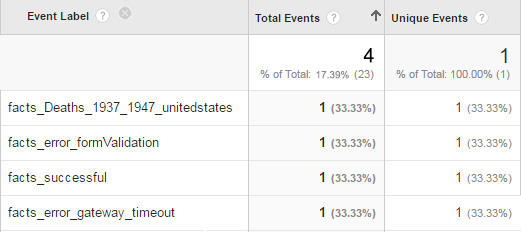
\includegraphics[scale=0.6]{10/04_factsEvents}
        \centering
        \caption{Exemple d'esdeveniments de la funcionalitat evolució d'esdeveniments}\label{img:factsEvents}
    \end{figure}

    A continuació, també citem els diferents exemples mostrats en la figura [] i hi afegim algun comentari.

    \begin{itemize}
        \item \textbf{Formulari incorrecte:} \emph{facts\_error\_formValidation}. Esdeveniment que s'envia quan la petició no s'ha arribat a processar perquè la configuració dels paràmetres no era correcta.
        \item \textbf{Petició llençada:} \emph{facts\_Deaths\_1937\_1947\_unitedstates}. Com es pot veure, quan es llança una petició contra l'API, també capturem el tipus d'esdeveniment cercat (defuncions), les dates per les quals s'ha cercat (1937-1947) i el país seleccionat (Estats Units).
        \item \textbf{Petició rebutjada:} \emph{facts\_error\_gateway\_timeout}. Aquest és un exemple dels esdeveniments que poden ser retornats quan l'API no ha pogut processar la petició.
        \item \textbf{Petició retornada amb èxit:} \emph{facts\_successful}. Esdeveniment que s'envia quan tot ha funcionat com s'esperava i l'API ha retornat resultats.
    \end{itemize}

    Els exemples d'esdeveniments anteriors, serveixen per demostrar el potencial que pot arribar a desencadenar una eina d'analítica web com Google Analytics.

    A part dels esdeveniments relatius a les funcionalitats implementades, que interactuen amb l'API de FamilySearch, també s'han implementat esdeveniments per controlar els intents d'identificació contra FamilySearch satisfactoris, les peticions de desconnexió, posicions dels exemples i propostes de projecte amb les que s'ha interactuat, interaccions amb la barra de navegació, posició de la persona seleccionada en la llista de resultats de la funcionalitat de cerca, etcètera.

    Tot i que el conjunt d'informació que s'ha exposat fins ara relativa a Google Analytics podria ser considerada simple, no creiem que sigui l'objectiu de la memòria entrar en molt més detall en les possibilitats d'una eina d'analítica web com aquesta, doncs realitzar una proposta profunda i exhaustiva de les possibilitats de monitoratge d'una web com la implementada, bé podria ser un projecte propi.

    \section{Optimitizació d'imatges}

    \paragraph{}
    Un dels elements més importants quan es desenvolupa una pàgina web és que aquesta carregui de forma ràpida. La diferència entre una pàgina lenta i una de ràpida, s'acaba traduint generalment en una pàgina web sense usuaris o amb usuaris.

    No era un objectiu del projecte fer una pàgina web el més optimitzada possible, ja que els coneixements tècnics necessaris requereixen temps per ser adquirits. No obstant això, sí que es volia realitzar les optimitzacions més típiques, que també solen ser les que endarrereixen més la càrrega de les pàgines web.

    Aquest apartat, cobra relativa importància, si tenim present que estem utilitzant un servei d'hostalatge gratuït i que per tant, la velocitat de resposta del servidor, no és de les millors del mercat.

    La manca d'optimització en les imatges sol ser un dels factors que més afecta a l'hora de carregar una pàgina web. Els programes de disseny utilitzats per generar imatges de gran qualitat, solen emmagatzemar més informació que la perceptible per l'ull humà, en circumstàncies normals.

    És per aquest motiu que optimitzar les imatges, els arxius més grans a descarregar de forma general en una web, esdevé un procés relativament comú.

    Per optimitzar les imatges de la nostra aplicació web s'ha utilitzat l'aplicació Optimizilla. Aquesta eina, penjada al núvol, utilitza una combinació de tècniques d'optimització i compressió amb pèrdues, per tal de reduir al màxim el pes d'imatges JPG i PNG, sense reduir el nivell de qualitat perceptible per l'ull humà.

    La utilització d'aquesta eina ha reduït, de forma aproximada, el 60-80\% del pes de totes les imatges que s'utilitzen en l'aplicació web. Fet considerable, si tenim en compte que no s'ha reduït la qualitat perceptible d'aquestes.

    \section{Hosting de l'aplicació}

    \paragraph{}
    Com ja s'ha indicat en el primer apartat d'aquesta secció de la memòria, l'aplicació es troba accessible a través del domini:

    \begin{displayquote}
        https://pfc-family-search.herokuapp.com/
    \end{displayquote}

    Hem escollit la plataforma Heroku per desplegar l'aplicació, ja que oferia un ampli ventall d'eines i documentació, que resultaven ideals per un desenvolupador novici de la plataforma Node.js.

    No obstant això, no van ser només aquestes facilitats i eines les que ens van portar a desplegar l'aplicació a Heroku, sinó també el fet que el seu pla de hosting gratuït s'ajustava en gran mesura al que el projecte requeria i en cas d'acabar necessitant més, sempre existia la possibilitat d'augmentar la capacitat de processat necessària.

    Les característiques que més ens van atreure de la plataforma Heroku es presenten d'una en una en els següents apartats.

    \subsection{Fàcil configuració}

    \paragraph{}
    Per una aplicació simple com la desenvolupada per aquest projecte, no fa falta canviar res en el codi de la nostra aplicació per tal de desplegar-la a Heroku. Només hem d'incloure un nou fitxer, a la carpeta arrel del projecte i amb el nom \emph{Procfile}, que indica el tipus d'aplicació i la comanda que ha ser utilitzada per tal d'iniciar-la.

    En el nostre cas, el fitxer \emph{Procfile} conte la següent línea de codi:

    \begin{displayquote}
        > web: node app.js
    \end{displayquote}


    \subsection{Fàcil desplegament al núvol}

    \paragraph{}
    La plataforma Heroku es troba molt ben integrada amb Github, l'eina que hem utilitzat per mantenir sincronitzats els desenvolupaments en les diferents estacions de treball. Gràcies a aquesta integració, Heroku disposa d'una comanda que ens permet afegir un remot, a la carpeta del nostre projecte.

    \begin{displayquote}
        > heroku git:remote -a pfc-family-search
    \end{displayquote}

    Un cop tenim el remot de Heroku configurat, de la mateixa forma que podem enviar el codi de la nostra estació de treball al núvol, el podem enviar a Heroku per tal de desplegar la nostra aplicació web. Això és tan fàcil com llençar la següent instrucció.

    \begin{displayquote}
        > git push heroku master
    \end{displayquote}


    \subsection{Entorn de proves local}

    \paragraph{}
    A part de l'entorn de proves local que podem configurar mitjançant la instal·lació de Node.js en el nostre sistema, Heroku també ens permet simular un entorn de producció Heroku, en l'àmbit local. S'aconsegueix mitjançant la següent instrucció:

    \begin{displayquote}
        > heroku local web
    \end{displayquote}

    Tot i que no aporta gaires diferències respecte a desplegar l'aplicació en local mitjançant Node.js de la forma convencional, pot esdevenir útil sota certes circumstàncies.


    \subsection{Decent versió gratuita}

    \paragraph{}
    Durant tot el procés de desenvolupament, l'aplicació es trobava sota el paquet de funcionalitats gratuït ofert per Heroku.

    Aquest ofereix les següents funcionalitats:

    \begin{itemize}
        \item Desplegament des de repositoris GIT.
        \item Actualitzacions automàtiques.
        \item Auto reparació d'aplicacions.
        \item Logs del sistema.
        \item Nombre de processos diferents suportats: 2
        \item 1000 hores mensuals de \emph{dyno} actius. L'aplicació s'adorm després de 30 minuts d'inactivitat.
        \item Dominis personalitzables.
        \item 512MB de RAM
    \end{itemize}


    \subsection{Fàcil escalatge de l'aplicació}

    \paragraph{}
    En cas que es desitgi millorar la capacitat de concurrència de l'aplicació, per poder rebre i processar més peticions en paral·lel i realitzar més processos diferents al mateix temps, aquesta és fàcilment escalable mitjançant la inclusió de nous \emph{dynos}.

    Els \emph{dynos} són els contenidors que executen les comandes dels usuaris. Per la nostra aplicació web, bàsicament es necessiten \emph{dynos} que processin el tràfic HTTP i HTTPS. Gràcies al fet que el nostre servidor és bastant simple (hem posat la lògica d'interacció amb l'API de FamilySearch a la capa del controlador) és probable que no faci falta augmentar el nombre de \emph{dynos} inicial.

    De totes maneres, aquest és fàcilment escalable mitjançant una simple comanda, sempre i quan el nostre pla contractat amb Heroku no sigui el gratuït. Si volem augmentar, per exemple, a 2 el nombre de \emph{dynos} disponibles, executaríem la següent comanda:

    \begin{displayquote}
        > heroku ps:scale web=2
    \end{displayquote}


    \chapter{Funcionalitats d'exemple amb FamilySearch}

    \section{Introducció a les funcionalitats implementades}

    \paragraph{}
    En aquesta secció de la memòria seran presentats els diferents exemples implementats, en la nostra aplicació web, que interactuen amb l'API de FamilySearch.

    Per cada una de les funcionalitat es proporcionarà una descripció adequada de la seva funció, detalls d'implementació, patrons d'usabilitat i recomanacions i exemples d'utilització si s'escau.

    Recordar també en aquest apartat, que publicar tot el codi implementat de les diferents funcionalitats és impossible, ja que només el controlador d'alguna d'elles, arriba a les quasi mil línies de codi.

    És per aquest motiu, que en els següents apartats, es mostraran només certes parts del codi, sempre simplificades, que creiem que poden resultar d'especial interès per tal de comprendre les bàsiques sota les quals funcionen les diferents funcionalitats. Com sempre, tot el codi font pot ser trobat a la pàgina de GitHub\footnote{https://github.com/sinh15/pfc-family-search}.

    \section{Identificació i desconnexió a l'API de FamilySearch}

    \subsection{Descripció de la funcionalitat}

\paragraph{}
La funcionalitat evolució temporal d'esdeveniments, permet als usuaris explorar el nombre d'instàncies de naixements, casaments i defuncions, enregistrades a les bases de dades de FamilySearch, per un país, al llarg d'un període d'onze anys.

Aquesta funcionalitat, probablement la més simple de les tres implementades, doncs reutilitza molta part del codi de les funcionalitats anteriors, és també una de les més interessants de cara a les diferents utilitzacions que si li poden donar.

Aquesta funcionalitat, de la mateixa forma que l'evolució geogràfica d'un cognom, utilitza la funció de conveniència del SDK, getResultsCount(), per millorar l’eficiència en l’obtenció de resultats i per tant, no entrarem a enumerar els seus avantatge una altre vegada.

La funcionalitat, llançarà un total d’onze crides al SDK, una per cada any de l’interval a considerar.

L'evolució temporal d'esdeveniments, permet a l'usuari configurar els següents tres paràmetres:

\begin{itemize}
    \item \textbf{Esdeveniment:} A seleccionar entre naixements, casaments o defuncions.
    \item \textbf{Localització:} Localització en la qual seran cercades les instàncies de l'esdeveniment seleccionat.
    \item \textbf{Any central:} Any central, del període d’onze anys, pel que es realitzarà la cerca. La funcionalitat genera l’interval +/- 5 anys, respecta l'any introduït. Així, per exemple, si introduïm l'any 1942, el rang d'anys utilitzat serà 1937-1947, ambdós inclosos.
\end{itemize}

Un cop el SDK retorna resultats per totes les consultes enviades, es pinta un gràfic de línies que mostra l'evolució del nombre d'instàncies de \emph{esdeveniment}, trobades al llarg del període seleccionat.

    \subsection{Detalls d'implementació}

    \input{./sections/11/02_connection/02_extraFiles/01_client}
    \input{./sections/11/02_connection/02_extraFiles/02_login}
    \input{./sections/11/02_connection/02_extraFiles/03_logout}

    \subsection{Aspectes d'usabilitat considerats}

    \paragraph{}
    Les funcions de connexió i desconnexió realitzen feina sense necessitat d'interacció per part de l'usuari i per tant, no s'han pogut tractar gaires aspectes d'usabilitat. No obstant això, sí que s'ha volgut informar a l'usuari de què s'està esperant la seva identificació amb FamilySearch, quan aquest prem el botó d'identificació.

    Quan el pop up d'identificació amb FamilySearch és mostrat, el contingut de la pàgina \emph{login.html} s'esvaeix i apareix la imatge animada, mostrada a la figura~\ref{fig:fsLoginWait}, que indica que s'està esperant una interacció per part de l'usuari. Quan l'usuari acaba el procés d'identificació, aquest és redirigit de forma automàtica a la pàgina d'exemples o a la pàgina principal en cas d'error.

    \begin{figure}[h]
        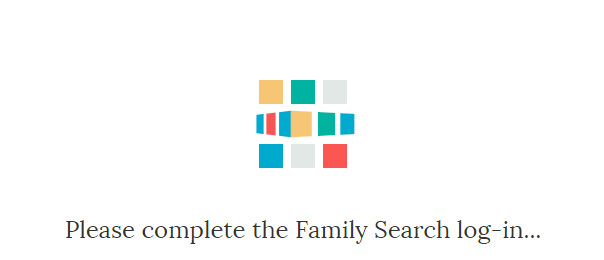
\includegraphics[scale=0.5]{11/01_loginLogout/02_waitingLogin}
        \centering
        \caption{Imatge animada mostrada mentre s'espera l'identificació de l'usuari}\label{fig:fsLoginWait}
    \end{figure}

    El segon aspecte d'usabilitat considerat, és que el botó de desconnectar-se només apareix, evidentment, si l'usuari es troba identificat.


    \section{Cerca de persones a l'arbre familiar}

    \subsection{Descripció de la funcionalitat}

\paragraph{}
La funcionalitat evolució temporal d'esdeveniments, permet als usuaris explorar el nombre d'instàncies de naixements, casaments i defuncions, enregistrades a les bases de dades de FamilySearch, per un país, al llarg d'un període d'onze anys.

Aquesta funcionalitat, probablement la més simple de les tres implementades, doncs reutilitza molta part del codi de les funcionalitats anteriors, és també una de les més interessants de cara a les diferents utilitzacions que si li poden donar.

Aquesta funcionalitat, de la mateixa forma que l'evolució geogràfica d'un cognom, utilitza la funció de conveniència del SDK, getResultsCount(), per millorar l’eficiència en l’obtenció de resultats i per tant, no entrarem a enumerar els seus avantatge una altre vegada.

La funcionalitat, llançarà un total d’onze crides al SDK, una per cada any de l’interval a considerar.

L'evolució temporal d'esdeveniments, permet a l'usuari configurar els següents tres paràmetres:

\begin{itemize}
    \item \textbf{Esdeveniment:} A seleccionar entre naixements, casaments o defuncions.
    \item \textbf{Localització:} Localització en la qual seran cercades les instàncies de l'esdeveniment seleccionat.
    \item \textbf{Any central:} Any central, del període d’onze anys, pel que es realitzarà la cerca. La funcionalitat genera l’interval +/- 5 anys, respecta l'any introduït. Així, per exemple, si introduïm l'any 1942, el rang d'anys utilitzat serà 1937-1947, ambdós inclosos.
\end{itemize}

Un cop el SDK retorna resultats per totes les consultes enviades, es pinta un gràfic de línies que mostra l'evolució del nombre d'instàncies de \emph{esdeveniment}, trobades al llarg del període seleccionat.

    \subsection{Recomanacions d'utilització}

    \paragraph{}
    Aquesta funcionalitat, no restringeix el nivell de localitzacions a utilitzar, de forma contrària a la funcionalitat d'expansió geogràfica d'un cognom i replica, de fet, el funcionament de les localitzacions  que s’introduïen en la funcionalitat de cerca.

    El paràmetre localització, per tant, accepta una gran diversitat de nivells d'especificació diferents, però per assegurar que la cerca produeix resultats, cal sempre introduir, com a mínim, el nivell de província o estat. De totes maneres, per l'exploració d'aquesta funcionalitat, es recomana introduir també el país o millor encara, cercar directament per un país.

    Una segona consideració a tenir en compte és que les bases de dades de FamilySearch no contenen, per tots els països, localitzacions i anys, la mateixa quantitat de registres. Per tant, utilitzar la funcionalitat en regions i períodes de temps rics en registres, produirà, amb alta probabilitat, resultats més interesants.

    \subsection{Detalls d'implementació}

    \paragraph{}
    Abans de destacar els detalls d'implementació d'aquesta funcionalitat, volem comentar, de la mateixa forma que per les dues funcionalitats anteriors, que només el controlador que gestiona la funcionalitat, està format per tres-centes línies de codi i en conseqüència, manca de sentit intentar representar totes les funcionalitats i aspectes d'aquesta en la memòria.

    El controlador encarregat del funcionament de l'evolució temporal d'esdeveniments és el fitxer \emph{facts.js}.

    \input{./sections/11/05_facts/03_extraFiles/01_formValidation}
    \input{./sections/11/05_facts/03_extraFiles/02_async}
    \input{./sections/11/05_facts/03_extraFiles/03_graphics}

    \subsection{Aspectes d'usabilitat considerats}

    \input{./sections/11/03_psearch/03_extraFiles/05_formLength}
    \input{./sections/11/03_psearch/03_extraFiles/06_formValidation}
    \input{./sections/11/03_psearch/03_extraFiles/07_loadingAnimation}
    \input{./sections/11/03_psearch/03_extraFiles/08_apiError}
    \input{./sections/11/03_psearch/03_extraFiles/09_arrows}
    \input{./sections/11/03_psearch/03_extraFiles/10_upArrows}
    \input{./sections/11/03_psearch/03_extraFiles/11_verticalAnimation}
    \input{./sections/11/03_psearch/03_extraFiles/12_stateRepresentation}

    \subsection{Principal interés d'ús}

\paragraph{}
El principal interès d'ús d'aquesta funcionalitat és explorar l'arbre familiar de FamilySearch i observar la diferent informació disponible relacionada a les persones retornades.




    % ending memory sections
    %\clearpage
	%\printglossaries{}

\end{document}
